\documentclass[10pt]{article} % For LaTeX2e
% \usepackage{tmlr}
% If accepted, instead use the following line for the camera-ready submission:
\usepackage[accepted]{tmlr}
% To de-anonymize and remove mentions to TMLR (for example for posting to preprint servers), instead use the following:
%\usepackage[preprint]{tmlr}

% Optional math commands from https://github.com/goodfeli/dlbook_notation.
%%%%% NEW MATH DEFINITIONS %%%%%

\usepackage{amsmath,amsfonts,bm}

% Mark sections of captions for referring to divisions of figures
\newcommand{\figleft}{{\em (Left)}}
\newcommand{\figcenter}{{\em (Center)}}
\newcommand{\figright}{{\em (Right)}}
\newcommand{\figtop}{{\em (Top)}}
\newcommand{\figbottom}{{\em (Bottom)}}
\newcommand{\captiona}{{\em (a)}}
\newcommand{\captionb}{{\em (b)}}
\newcommand{\captionc}{{\em (c)}}
\newcommand{\captiond}{{\em (d)}}

% Highlight a newly defined term
\newcommand{\newterm}[1]{{\bf #1}}


% Figure reference, lower-case.
\def\figref#1{figure~\ref{#1}}
% Figure reference, capital. For start of sentence
\def\Figref#1{Figure~\ref{#1}}
\def\twofigref#1#2{figures \ref{#1} and \ref{#2}}
\def\quadfigref#1#2#3#4{figures \ref{#1}, \ref{#2}, \ref{#3} and \ref{#4}}
% Section reference, lower-case.
\def\secref#1{section~\ref{#1}}
% Section reference, capital.
\def\Secref#1{Section~\ref{#1}}
% Reference to two sections.
\def\twosecrefs#1#2{sections \ref{#1} and \ref{#2}}
% Reference to three sections.
\def\secrefs#1#2#3{sections \ref{#1}, \ref{#2} and \ref{#3}}
% Reference to an equation, lower-case.
% \def\eqref#1{equation~\ref{#1}}
\def\eqref#1{(\ref{#1})}
% Reference to an equation, upper case
\def\Eqref#1{Equation~\ref{#1}}
% A raw reference to an equation---avoid using if possible
\def\plaineqref#1{\ref{#1}}
% Reference to a chapter, lower-case.
\def\chapref#1{chapter~\ref{#1}}
% Reference to an equation, upper case.
\def\Chapref#1{Chapter~\ref{#1}}
% Reference to a range of chapters
\def\rangechapref#1#2{chapters\ref{#1}--\ref{#2}}
% Reference to an algorithm, lower-case.
\def\algref#1{algorithm~\ref{#1}}
% Reference to an algorithm, upper case.
\def\Algref#1{Algorithm~\ref{#1}}
\def\twoalgref#1#2{algorithms \ref{#1} and \ref{#2}}
\def\Twoalgref#1#2{Algorithms \ref{#1} and \ref{#2}}
% Reference to a part, lower case
\def\partref#1{part~\ref{#1}}
% Reference to a part, upper case
\def\Partref#1{Part~\ref{#1}}
\def\twopartref#1#2{parts \ref{#1} and \ref{#2}}

\def\ceil#1{\lceil #1 \rceil}
\def\floor#1{\lfloor #1 \rfloor}
\def\1{\bm{1}}
\newcommand{\train}{\mathcal{D}}
\newcommand{\valid}{\mathcal{D_{\mathrm{valid}}}}
\newcommand{\test}{\mathcal{D_{\mathrm{test}}}}

\def\eps{{\epsilon}}


% Random variables
\def\reta{{\textnormal{$\eta$}}}
\def\ra{{\textnormal{a}}}
\def\rb{{\textnormal{b}}}
\def\rc{{\textnormal{c}}}
\def\rd{{\textnormal{d}}}
\def\re{{\textnormal{e}}}
\def\rf{{\textnormal{f}}}
\def\rg{{\textnormal{g}}}
\def\rh{{\textnormal{h}}}
\def\ri{{\textnormal{i}}}
\def\rj{{\textnormal{j}}}
\def\rk{{\textnormal{k}}}
\def\rl{{\textnormal{l}}}
% rm is already a command, just don't name any random variables m
\def\rn{{\textnormal{n}}}
\def\ro{{\textnormal{o}}}
\def\rp{{\textnormal{p}}}
\def\rq{{\textnormal{q}}}
\def\rr{{\textnormal{r}}}
\def\rs{{\textnormal{s}}}
\def\rt{{\textnormal{t}}}
\def\ru{{\textnormal{u}}}
\def\rv{{\textnormal{v}}}
\def\rw{{\textnormal{w}}}
\def\rx{{\textnormal{x}}}
\def\ry{{\textnormal{y}}}
\def\rz{{\textnormal{z}}}

% Random vectors
\def\rvepsilon{{\mathbf{\epsilon}}}
\def\rvtheta{{\mathbf{\theta}}}
\def\rva{{\mathbf{a}}}
\def\rvb{{\mathbf{b}}}
\def\rvc{{\mathbf{c}}}
\def\rvd{{\mathbf{d}}}
\def\rve{{\mathbf{e}}}
\def\rvf{{\mathbf{f}}}
\def\rvg{{\mathbf{g}}}
\def\rvh{{\mathbf{h}}}
\def\rvu{{\mathbf{i}}}
\def\rvj{{\mathbf{j}}}
\def\rvk{{\mathbf{k}}}
\def\rvl{{\mathbf{l}}}
\def\rvm{{\mathbf{m}}}
\def\rvn{{\mathbf{n}}}
\def\rvo{{\mathbf{o}}}
\def\rvp{{\mathbf{p}}}
\def\rvq{{\mathbf{q}}}
\def\rvr{{\mathbf{r}}}
\def\rvs{{\mathbf{s}}}
\def\rvt{{\mathbf{t}}}
\def\rvu{{\mathbf{u}}}
\def\rvv{{\mathbf{v}}}
\def\rvw{{\mathbf{w}}}
\def\rvx{{\mathbf{x}}}
\def\rvy{{\mathbf{y}}}
\def\rvz{{\mathbf{z}}}

% Elements of random vectors
\def\erva{{\textnormal{a}}}
\def\ervb{{\textnormal{b}}}
\def\ervc{{\textnormal{c}}}
\def\ervd{{\textnormal{d}}}
\def\erve{{\textnormal{e}}}
\def\ervf{{\textnormal{f}}}
\def\ervg{{\textnormal{g}}}
\def\ervh{{\textnormal{h}}}
\def\ervi{{\textnormal{i}}}
\def\ervj{{\textnormal{j}}}
\def\ervk{{\textnormal{k}}}
\def\ervl{{\textnormal{l}}}
\def\ervm{{\textnormal{m}}}
\def\ervn{{\textnormal{n}}}
\def\ervo{{\textnormal{o}}}
\def\ervp{{\textnormal{p}}}
\def\ervq{{\textnormal{q}}}
\def\ervr{{\textnormal{r}}}
\def\ervs{{\textnormal{s}}}
\def\ervt{{\textnormal{t}}}
\def\ervu{{\textnormal{u}}}
\def\ervv{{\textnormal{v}}}
\def\ervw{{\textnormal{w}}}
\def\ervx{{\textnormal{x}}}
\def\ervy{{\textnormal{y}}}
\def\ervz{{\textnormal{z}}}

% Random matrices
\def\rmA{{\mathbf{A}}}
\def\rmB{{\mathbf{B}}}
\def\rmC{{\mathbf{C}}}
\def\rmD{{\mathbf{D}}}
\def\rmE{{\mathbf{E}}}
\def\rmF{{\mathbf{F}}}
\def\rmG{{\mathbf{G}}}
\def\rmH{{\mathbf{H}}}
\def\rmI{{\mathbf{I}}}
\def\rmJ{{\mathbf{J}}}
\def\rmK{{\mathbf{K}}}
\def\rmL{{\mathbf{L}}}
\def\rmM{{\mathbf{M}}}
\def\rmN{{\mathbf{N}}}
\def\rmO{{\mathbf{O}}}
\def\rmP{{\mathbf{P}}}
\def\rmQ{{\mathbf{Q}}}
\def\rmR{{\mathbf{R}}}
\def\rmS{{\mathbf{S}}}
\def\rmT{{\mathbf{T}}}
\def\rmU{{\mathbf{U}}}
\def\rmV{{\mathbf{V}}}
\def\rmW{{\mathbf{W}}}
\def\rmX{{\mathbf{X}}}
\def\rmY{{\mathbf{Y}}}
\def\rmZ{{\mathbf{Z}}}

% Elements of random matrices
\def\ermA{{\textnormal{A}}}
\def\ermB{{\textnormal{B}}}
\def\ermC{{\textnormal{C}}}
\def\ermD{{\textnormal{D}}}
\def\ermE{{\textnormal{E}}}
\def\ermF{{\textnormal{F}}}
\def\ermG{{\textnormal{G}}}
\def\ermH{{\textnormal{H}}}
\def\ermI{{\textnormal{I}}}
\def\ermJ{{\textnormal{J}}}
\def\ermK{{\textnormal{K}}}
\def\ermL{{\textnormal{L}}}
\def\ermM{{\textnormal{M}}}
\def\ermN{{\textnormal{N}}}
\def\ermO{{\textnormal{O}}}
\def\ermP{{\textnormal{P}}}
\def\ermQ{{\textnormal{Q}}}
\def\ermR{{\textnormal{R}}}
\def\ermS{{\textnormal{S}}}
\def\ermT{{\textnormal{T}}}
\def\ermU{{\textnormal{U}}}
\def\ermV{{\textnormal{V}}}
\def\ermW{{\textnormal{W}}}
\def\ermX{{\textnormal{X}}}
\def\ermY{{\textnormal{Y}}}
\def\ermZ{{\textnormal{Z}}}

% Vectors
\def\vzero{{\bm{0}}}
\def\vone{{\bm{1}}}
\def\vmu{{\bm{\mu}}}
\def\vtheta{{\bm{\theta}}}
\def\va{{\bm{a}}}
\def\vb{{\bm{b}}}
\def\vc{{\bm{c}}}
\def\vd{{\bm{d}}}
\def\ve{{\bm{e}}}
\def\vf{{\bm{f}}}
\def\vg{{\bm{g}}}
\def\vh{{\bm{h}}}
\def\vi{{\bm{i}}}
\def\vj{{\bm{j}}}
\def\vk{{\bm{k}}}
\def\vl{{\bm{l}}}
\def\vm{{\bm{m}}}
\def\vn{{\bm{n}}}
\def\vo{{\bm{o}}}
\def\vp{{\bm{p}}}
\def\vq{{\bm{q}}}
\def\vr{{\bm{r}}}
\def\vs{{\bm{s}}}
\def\vt{{\bm{t}}}
\def\vu{{\bm{u}}}
\def\vv{{\bm{v}}}
\def\vw{{\bm{w}}}
\def\vx{{\bm{x}}}
\def\vy{{\bm{y}}}
\def\vz{{\bm{z}}}

% Elements of vectors
\def\evalpha{{\alpha}}
\def\evbeta{{\beta}}
\def\evepsilon{{\epsilon}}
\def\evlambda{{\lambda}}
\def\evomega{{\omega}}
\def\evmu{{\mu}}
\def\evpsi{{\psi}}
\def\evsigma{{\sigma}}
\def\evtheta{{\theta}}
\def\eva{{a}}
\def\evb{{b}}
\def\evc{{c}}
\def\evd{{d}}
\def\eve{{e}}
\def\evf{{f}}
\def\evg{{g}}
\def\evh{{h}}
\def\evi{{i}}
\def\evj{{j}}
\def\evk{{k}}
\def\evl{{l}}
\def\evm{{m}}
\def\evn{{n}}
\def\evo{{o}}
\def\evp{{p}}
\def\evq{{q}}
\def\evr{{r}}
\def\evs{{s}}
\def\evt{{t}}
\def\evu{{u}}
\def\evv{{v}}
\def\evw{{w}}
\def\evx{{x}}
\def\evy{{y}}
\def\evz{{z}}

% Matrix
\def\mA{{\bm{A}}}
\def\mB{{\bm{B}}}
\def\mC{{\bm{C}}}
\def\mD{{\bm{D}}}
\def\mE{{\bm{E}}}
\def\mF{{\bm{F}}}
\def\mG{{\bm{G}}}
\def\mH{{\bm{H}}}
\def\mI{{\bm{I}}}
\def\mJ{{\bm{J}}}
\def\mK{{\bm{K}}}
\def\mL{{\bm{L}}}
\def\mM{{\bm{M}}}
\def\mN{{\bm{N}}}
\def\mO{{\bm{O}}}
\def\mP{{\bm{P}}}
\def\mQ{{\bm{Q}}}
\def\mR{{\bm{R}}}
\def\mS{{\bm{S}}}
\def\mT{{\bm{T}}}
\def\mU{{\bm{U}}}
\def\mV{{\bm{V}}}
\def\mW{{\bm{W}}}
\def\mX{{\bm{X}}}
\def\mY{{\bm{Y}}}
\def\mZ{{\bm{Z}}}
\def\mBeta{{\bm{\beta}}}
\def\mPhi{{\bm{\Phi}}}
\def\mLambda{{\bm{\Lambda}}}
\def\mSigma{{\bm{\Sigma}}}

% Tensor
\DeclareMathAlphabet{\mathsfit}{\encodingdefault}{\sfdefault}{m}{sl}
\SetMathAlphabet{\mathsfit}{bold}{\encodingdefault}{\sfdefault}{bx}{n}
\newcommand{\tens}[1]{\bm{\mathsfit{#1}}}
\def\tA{{\tens{A}}}
\def\tB{{\tens{B}}}
\def\tC{{\tens{C}}}
\def\tD{{\tens{D}}}
\def\tE{{\tens{E}}}
\def\tF{{\tens{F}}}
\def\tG{{\tens{G}}}
\def\tH{{\tens{H}}}
\def\tI{{\tens{I}}}
\def\tJ{{\tens{J}}}
\def\tK{{\tens{K}}}
\def\tL{{\tens{L}}}
\def\tM{{\tens{M}}}
\def\tN{{\tens{N}}}
\def\tO{{\tens{O}}}
\def\tP{{\tens{P}}}
\def\tQ{{\tens{Q}}}
\def\tR{{\tens{R}}}
\def\tS{{\tens{S}}}
\def\tT{{\tens{T}}}
\def\tU{{\tens{U}}}
\def\tV{{\tens{V}}}
\def\tW{{\tens{W}}}
\def\tX{{\tens{X}}}
\def\tY{{\tens{Y}}}
\def\tZ{{\tens{Z}}}


% Graph
\def\gA{{\mathcal{A}}}
\def\gB{{\mathcal{B}}}
\def\gC{{\mathcal{C}}}
\def\gD{{\mathcal{D}}}
\def\gE{{\mathcal{E}}}
\def\gF{{\mathcal{F}}}
\def\gG{{\mathcal{G}}}
\def\gH{{\mathcal{H}}}
\def\gI{{\mathcal{I}}}
\def\gJ{{\mathcal{J}}}
\def\gK{{\mathcal{K}}}
\def\gL{{\mathcal{L}}}
\def\gM{{\mathcal{M}}}
\def\gN{{\mathcal{N}}}
\def\gO{{\mathcal{O}}}
\def\gP{{\mathcal{P}}}
\def\gQ{{\mathcal{Q}}}
\def\gR{{\mathcal{R}}}
\def\gS{{\mathcal{S}}}
\def\gT{{\mathcal{T}}}
\def\gU{{\mathcal{U}}}
\def\gV{{\mathcal{V}}}
\def\gW{{\mathcal{W}}}
\def\gX{{\mathcal{X}}}
\def\gY{{\mathcal{Y}}}
\def\gZ{{\mathcal{Z}}}

% Sets
\def\sA{{\mathbb{A}}}
\def\sB{{\mathbb{B}}}
\def\sC{{\mathbb{C}}}
\def\sD{{\mathbb{D}}}
% Don't use a set called E, because this would be the same as our symbol
% for expectation.
\def\sF{{\mathbb{F}}}
\def\sG{{\mathbb{G}}}
\def\sH{{\mathbb{H}}}
\def\sI{{\mathbb{I}}}
\def\sJ{{\mathbb{J}}}
\def\sK{{\mathbb{K}}}
\def\sL{{\mathbb{L}}}
\def\sM{{\mathbb{M}}}
\def\sN{{\mathbb{N}}}
\def\sO{{\mathbb{O}}}
\def\sP{{\mathbb{P}}}
\def\sQ{{\mathbb{Q}}}
\def\sR{{\mathbb{R}}}
\def\sS{{\mathbb{S}}}
\def\sT{{\mathbb{T}}}
\def\sU{{\mathbb{U}}}
\def\sV{{\mathbb{V}}}
\def\sW{{\mathbb{W}}}
\def\sX{{\mathbb{X}}}
\def\sY{{\mathbb{Y}}}
\def\sZ{{\mathbb{Z}}}

% Entries of a matrix
\def\emLambda{{\Lambda}}
\def\emA{{A}}
\def\emB{{B}}
\def\emC{{C}}
\def\emD{{D}}
\def\emE{{E}}
\def\emF{{F}}
\def\emG{{G}}
\def\emH{{H}}
\def\emI{{I}}
\def\emJ{{J}}
\def\emK{{K}}
\def\emL{{L}}
\def\emM{{M}}
\def\emN{{N}}
\def\emO{{O}}
\def\emP{{P}}
\def\emQ{{Q}}
\def\emR{{R}}
\def\emS{{S}}
\def\emT{{T}}
\def\emU{{U}}
\def\emV{{V}}
\def\emW{{W}}
\def\emX{{X}}
\def\emY{{Y}}
\def\emZ{{Z}}
\def\emSigma{{\Sigma}}

% entries of a tensor
% Same font as tensor, without \bm wrapper
\newcommand{\etens}[1]{\mathsfit{#1}}
\def\etLambda{{\etens{\Lambda}}}
\def\etA{{\etens{A}}}
\def\etB{{\etens{B}}}
\def\etC{{\etens{C}}}
\def\etD{{\etens{D}}}
\def\etE{{\etens{E}}}
\def\etF{{\etens{F}}}
\def\etG{{\etens{G}}}
\def\etH{{\etens{H}}}
\def\etI{{\etens{I}}}
\def\etJ{{\etens{J}}}
\def\etK{{\etens{K}}}
\def\etL{{\etens{L}}}
\def\etM{{\etens{M}}}
\def\etN{{\etens{N}}}
\def\etO{{\etens{O}}}
\def\etP{{\etens{P}}}
\def\etQ{{\etens{Q}}}
\def\etR{{\etens{R}}}
\def\etS{{\etens{S}}}
\def\etT{{\etens{T}}}
\def\etU{{\etens{U}}}
\def\etV{{\etens{V}}}
\def\etW{{\etens{W}}}
\def\etX{{\etens{X}}}
\def\etY{{\etens{Y}}}
\def\etZ{{\etens{Z}}}

% The true underlying data generating distribution
\newcommand{\pdata}{p_{\rm{data}}}
% The empirical distribution defined by the training set
\newcommand{\ptrain}{\hat{p}_{\rm{data}}}
\newcommand{\Ptrain}{\hat{P}_{\rm{data}}}
% The model distribution
\newcommand{\pmodel}{p_{\rm{model}}}
\newcommand{\Pmodel}{P_{\rm{model}}}
\newcommand{\ptildemodel}{\tilde{p}_{\rm{model}}}
% Stochastic autoencoder distributions
\newcommand{\pencode}{p_{\rm{encoder}}}
\newcommand{\pdecode}{p_{\rm{decoder}}}
\newcommand{\precons}{p_{\rm{reconstruct}}}

\newcommand{\laplace}{\mathrm{Laplace}} % Laplace distribution

\newcommand{\E}{\mathbb{E}}
\newcommand{\Ls}{\mathcal{L}}
\newcommand{\R}{\mathbb{R}}
\newcommand{\emp}{\tilde{p}}
\newcommand{\lr}{\alpha}
\newcommand{\reg}{\lambda}
\newcommand{\rect}{\mathrm{rectifier}}
\newcommand{\softmax}{\mathrm{softmax}}
\newcommand{\sigmoid}{\sigma}
\newcommand{\softplus}{\zeta}
\newcommand{\KL}{D_{\mathrm{KL}}}
\newcommand{\Var}{\mathrm{Var}}
\newcommand{\standarderror}{\mathrm{SE}}
\newcommand{\Cov}{\mathrm{Cov}}
% Wolfram Mathworld says $L^2$ is for function spaces and $\ell^2$ is for vectors
% But then they seem to use $L^2$ for vectors throughout the site, and so does
% wikipedia.
\newcommand{\normlzero}{L^0}
\newcommand{\normlone}{L^1}
\newcommand{\normltwo}{L^2}
\newcommand{\normlp}{L^p}
\newcommand{\normmax}{L^\infty}

\newcommand{\parents}{Pa} % See usage in notation.tex. Chosen to match Daphne's book.

\DeclareMathOperator*{\argmax}{arg\,max}
\DeclareMathOperator*{\argmin}{arg\,min}

\DeclareMathOperator{\sign}{sign}
\DeclareMathOperator{\Tr}{Tr}
\let\ab\allowbreak

\usepackage{amsmath}
\usepackage{amsfonts}
\usepackage{amssymb}
\usepackage[protrusion=true,tracking=true,kerning=true,expansion,final]{microtype} 

% Breaks links at "/"
\usepackage[pagebackref=true,breaklinks=true,colorlinks,bookmarks=true]{hyperref}

\definecolor{citecolor}{rgb}{.259,.659,1}
\definecolor{mydarkblue}{rgb}{0,0.08,0.45}
\definecolor{urlcolor}{rgb}{0,.145,.698}
\definecolor{linkcolor}{rgb}{0.01,0.31,.65}
\hypersetup{
    colorlinks=true,
    breaklinks=true,  %
    bookmarksnumbered=true,
    linkcolor=linkcolor,
    citecolor=citecolor,
    filecolor=mydarkblue,
    urlcolor=urlcolor,
    pdftitle={StarCoder: may the source be with you!},
    pdfpagemode=FullScreen,
    pdfview=FitH
    }

\renewcommand*{\backref}[1]{} %
\renewcommand*{\backrefalt}[4]{%
	\ifcase #1 %
	\or
	(cited on p. #2)%
	\else
	(cited on pp. #2)%
	\fi
}
\makeatletter
\renewcommand{\@biblabel}[1]{#1.}
\makeatother
% Also break links at "-"
\def\UrlBreaks{\do\/\do-}


\usepackage{multicol}
\usepackage{booktabs}
\usepackage{graphicx}
\usepackage{multirow}
\usepackage{pifont}% 
\usepackage{listings}
\usepackage{tabularx}
\usepackage{fancyvrb}

% dfried: for nicer monospace fonts (but feel free to remove if dispreferred)
\usepackage{inconsolata}

% For inparaenum, which gives \item within a paragraph.
\usepackage{paralist}

\lstset{
  basicstyle=\ttfamily,
  columns=fullflexible,
  frame=single,
  breaklines=true,
  inputencoding=utf8,
  showstringspaces=false,
}

\usepackage{subcaption}
\usepackage{xparse}
\NewDocumentCommand\emojistar{}{
        
\includegraphics[scale=0.24]{figures/staremoji.png}
}
\NewDocumentCommand\emojidizzy{}{
        
\includegraphics[scale=0.16]{figures/dizzy_emoji.png}
}
% http://ctan.org/pkg/pifont
\newcommand{\cmark}{\ding{51}}%f
\newcommand{\xmark}{\ding{55}}%


\newcommand\ez[1]{\textcolor{brown}{(\textbf{Evgenii}: #1)}} % Adds comment, will paint the text in brown
\newcommand\red[1]{\textcolor{red}{#1}} 

\newcommand{\cpp}{C\texttt{++}}

% dfried: added to make multi-row entries in table headers easier
\newcommand*{\thead}[1]{%
\multicolumn{1}{c}{\begin{tabular}{@{}c@{}}#1\end{tabular}}}

\tolerance=1000
\hbadness=2000
\vbadness=\maxdimen
\sloppy 


%%FIGURES CONTROL%%
\renewcommand{\topfraction}{0.99}
\renewcommand{\textfraction}{.01}
\renewcommand{\floatpagefraction}{0.99}
\renewcommand{\dblfloatpagefraction}{0.99}
\setcounter{dbltopnumber}{2}  
\setcounter{topnumber}{2}  
\setcounter{bottomnumber}{2} 
\setcounter{totalnumber}{3}


\renewcommand{\textfraction}{0.003}
%\renewcommand{\floatpagefraction}{0.997}
% \title{Formatting Instructions for TMLR \\Journal Submissions}

% Authors must not appear in the submitted version. They should be hidden
% as long as the tmlr package is used without the [accepted] or [preprint] options.
% Non-anonymous submissions will be rejected without review.

\usepackage{float}
\newfloat{lstfloat}{htbp}{lop}
\floatname{lstfloat}{Listing}
\def\lstfloatautorefname{Listing} % needed for hyperref/auroref

\title{\emojidizzy StarCoder: may the source be with you! }


\def\month{12}  % Insert correct month for camera-ready version
\def\year{2023} % Insert correct year for camera-ready version
\def\openreview{\url{https://openreview.net/forum?id=KoFOg41haE}} % Insert correct link to OpenReview for camera-ready version


\begin{document}
\maketitle
\vspace{-6.5em}
\begin{center}
\textbf{Raymond Li}$^2$\quad
\textbf{Loubna Ben Allal}$^1$\quad
\textbf{Yangtian Zi}$^4$\quad
\textbf{Niklas Muennighoff}$^1$\quad
\textbf{Denis Kocetkov}$^2$\quad
\textbf{Chenghao Mou}$^5$\quad
\textbf{Marc Marone}$^8$\quad
\textbf{Christopher Akiki}$^{9,10}$\quad
\textbf{Jia Li}$^5$\quad
\textbf{Jenny Chim}$^{11}$\quad
\textbf{Qian Liu}$^{13}$\quad
\textbf{Evgenii Zheltonozhskii}$^{14}$\quad
\textbf{Terry Yue Zhuo}$^{15,16}$\quad
\textbf{Thomas Wang}$^1$\quad
\textbf{Olivier Dehaene}$^1$\quad
\textbf{Mishig Davaadorj}$^1$\quad
\textbf{Joel Lamy-Poirier}$^2$\quad
\textbf{João Monteiro}$^2$\quad
\textbf{Oleh Shliazhko}$^2$\quad
\textbf{Nicolas Gontier}$^2$\quad
\textbf{Nicholas Meade}$^{6,17}$\quad
\textbf{Armel Zebaze}$^1$\quad
\textbf{Ming-Ho Yee}$^4$\quad
\textbf{Logesh Kumar Umapathi}$^{18}$\quad
\textbf{Jian Zhu}$^{19}$\quad
\textbf{Benjamin Lipkin}$^{20}$\quad
\textbf{Muhtasham Oblokulov}$^{21}$\quad
\textbf{Zhiruo Wang}$^7$\quad
\textbf{Rudra Murthy}$^{22}$\quad
\textbf{Jason Stillerman}$^{23}$\quad
\textbf{Siva Sankalp Patel}$^{22}$\quad
\textbf{Dmitry Abulkhanov}$^5$\quad
\textbf{Marco Zocca}$^{24}$\quad
\textbf{Manan Dey}$^{25}$\quad
\textbf{Zhihan Zhang}$^{26}$\quad
\textbf{Nour Fahmy}$^{27}$\quad
\textbf{Urvashi Bhattacharyya}$^{28}$\quad
\textbf{Wenhao Yu}$^{26}$\quad
\textbf{Swayam Singh}$^{30}$\quad
\textbf{Sasha Luccioni}$^1$\quad
\textbf{Paulo Villegas}$^{31}$\quad
\textbf{Maxim Kunakov}$^{32}$\quad
\textbf{Fedor Zhdanov}$^{32}$\quad
\textbf{Manuel Romero}$^5$\quad
\textbf{Tony Lee}$^{33}$\quad
\textbf{Nadav Timor}$^{34}$\quad
\textbf{Jennifer Ding}$^{35}$\quad
\textbf{Claire Schlesinger}$^{4}$\quad
\\\textbf{Hailey Schoelkopf}$^{37}$\quad
\textbf{Jan Ebert}$^{38}$\quad
\textbf{Tri Dao}$^{33}$\quad
\textbf{Mayank Mishra}$^{22}$\quad
\textbf{Alex Gu}$^{20}$\quad
\textbf{Jennifer Robinson}$^3$\quad
\textbf{Carolyn Jane Anderson}$^{36}$\quad
\textbf{Brendan Dolan-Gavitt}$^{29}$\quad
\textbf{Danish Contractor}$^5$\quad
\textbf{Siva Reddy}$^{2,6}$\quad
\textbf{Daniel Fried}$^7$\quad
\textbf{Dzmitry Bahdanau}$^2$\quad
\textbf{Yacine Jernite}$^1$\quad
\textbf{Carlos Muñoz Ferrandis}$^1$\quad 
\textbf{Sean Hughes}$^3$\quad
\textbf{Thomas Wolf}$^1$\quad
\textbf{Arjun Guha}$^{4,12}$\quad
\\\textbf{Leandro von Werra}$^{1, \star}$\quad
\textbf{Harm de Vries}$^{2, \star}$\quad

% Affiliation
$^{1}$Hugging~Face \quad
$^{2}$ServiceNow Research\quad
$^{3}$ServiceNow\quad
$^{4}$Northeastern University\quad
$^{5}$Independent\quad
$^{6}$Mila\quad
$^{7}$Carnegie Mellon University\quad
$^{8}$Johns Hopkins University\quad
$^{9}$Leipzig University\quad
$^{10}$ScaDS.AI\quad
$^{11}$Queen Mary University of London\quad
$^{12}$Roblox\quad
$^{13}$Sea AI Lab\quad
$^{14}$Technion -- Israel Institute of Technology\quad
$^{15}$Monash University\quad
$^{16}$CSIRO's Data61\quad
$^{17}$McGill University\quad
$^{18}$Saama AI Research Lab\quad
$^{19}$University of British Columbia\quad
$^{20}$MIT\quad
$^{21}$Technical University of Munich\quad
$^{22}$IBM Research\quad
$^{23}$University of Vermont\quad
$^{24}$UnfoldML\quad
$^{25}$SAP\quad
$^{26}$University of Notre Dame\quad
$^{27}$Columbia University\quad
$^{28}$Discover Dollar Pvt Ltd\quad
$^{29}$NYU\quad
$^{30}$University of Allahabad\quad
$^{31}$Telefonica I+D\quad
$^{32}$Toloka\quad
$^{33}$Stanford University\quad
$^{34}$Weizmann Institute of Science\quad
$^{35}$The Alan Turing Institute\quad
$^{36}$Wellesley College\quad
$^{37}$Eleuther AI\quad
$^{38}$Forschungszentrum J{\"u}lich\quad

Corresponding authors ($\star$) can be contacted at \href{contact@bigcode-project.org}{contact@bigcode-project.org}\\
\vspace{0.5cm}
{\bf Reviewed on OpenReview:} \openreview
\end{center}

\begin{abstract}
The BigCode community, an open-scientific collaboration working on the responsible development of Large Language Models for Code (Code LLMs), introduces StarCoder and StarCoderBase: 15.5B parameter models with 8K context length, infilling capabilities and fast large-batch inference enabled by multi-query attention. StarCoderBase is trained on 1 trillion tokens sourced from The Stack~\citep{Kocetkov2022TheStack}, a large collection of permissively licensed GitHub repositories with inspection tools and an opt-out process. We fine-tuned StarCoderBase on 35B Python tokens, resulting in the creation of StarCoder. We perform the most comprehensive evaluation of Code LLMs to date and show that StarCoderBase outperforms every open Code LLM that supports multiple programming languages and matches or outperforms the OpenAI code-cushman-001 model. 
Furthermore, StarCoder outperforms every model that is fine-tuned on Python
% , can be prompted to achieve 40\% pass@1 on HumanEval, 
and still retains its performance on other programming languages.
We take several important steps towards a safe open-access model release, including an improved PII redaction pipeline and a novel attribution tracing tool, and make the StarCoder models publicly available under a more commercially viable version of the Open Responsible AI Model license. 
\end{abstract}

% Large Language Models \citep[LLMs;][]{brown2020language, chen2021codex,chowdhery2022palm,zhang2022opt,openai2023gpt4}, such as OpenAI's ChatGPT, are taking the world by storm. Within a mere two months of launching, ChatGPT has amassed over 100~million users, making it the fastest-growing internet application in history~\citep{guardian2023chatgpt}. Similarly, Microsoft’s Copilot, an LLM designed for coding applications, has attracted over 1~million~professional developers~\citep{euronews2023copilot} and can accelerate coding tasks by up to~55\%~\citep{kalliamvakou2022copilot}. 

\section{Introduction}
\vspace{-0.1cm}
Generative AI and large language models \citep[LLMs;][]{brown2020language, chen2021codex,chowdhery2022palm,zhang2022opt,openai2023gpt4} are predicted to significantly impact the workforce in the coming years~\citep{eloundou2023gpts, stanford2022foundation,wef2023futureofjobs} by boosting worker productivity.  
LLMs trained on code (Code LLMs) have seen particularly fast adoption: Microsoft’s Copilot has attracted over 1~million~professional developers~\citep{euronews2023copilot}
% and can accelerate coding tasks by up to~55\%~\citep{kalliamvakou2022copilot}, 
and GitHub reports that Copilot users rely on it to produce 35\% of the code they write for some languages~\citep{thompson-2022-copilot-stats}.
However, the development and use of LLMs has raised concerns of copyright, privacy, and openness.

% *Copyright concerns*
% Some safety concerns, such as generating false information or amplifying existing biases, are being addressed after training by using various techniques to better ``align'' the LLM with human values~\citep{stiennon2020learning,bai2022training,perez2022red}. 
Copyright concerns arise in many jurisdictions, including the U.S.\ and E.U.\,, regarding the rights of content creators whose public data is used to train language models. %This data is subject to copyright laws in many jurisdictions, including the U.S.\ and E.U..
It has been questioned whether machine learning models trained on such data fall under fair-use doctrine in the U.S.~\citep{kuhn2022copilot,butterick2022copilot,rothchild2022copyright}, with fair use being most likely when the model generates novel content dissimilar to any copyrighted training data~\citep{lemley2020fair,levendowski2018copyright}. 
% It has been questioned whether machine learning models trained on such data fall under exemptions such as the fair-use doctrine in the U.S.~\citep{kuhn2022copilot,butterick2022copilot,rothchild2022copyright}. It is likely considered fair use when a model generates novel content that is not in the training set, as it is a transformative use of the copyrighted material~\citep{lemley2020fair}. However, if the model produces output similar to copyrighted data, particularly in scenarios that affect the economic market of the content creators, fair use may no longer apply~\citep{levendowski2018copyright}. 
\citet{henderson2023foundation}, therefore, suggest LLM developers should provide additional tools to ensure these models comply with current copyright laws. It is important to mention that these legal issues are not only the subject of scholarly debates: lawsuits have already been filed against GitHub Copilot~\citep{DOE1vGitHub} as well as Stable Diffusion~\citep{stablediffusion_lawsuit}.%, a text-to-image tool from Stability~AI. 

% *Privacy concerns*
Concerns about personal information led Italy to temporarily ban ChatGPT and launch an ongoing investigation into OpenAI's compliance with the E.U.'s General Data Protection Regulation~(GDPR)~\citep{bbc2023chatgpt_ban}. According to these regulations~\citep{eu2018gdpr,lomas2023gdpr_llms}, organizations that process personal information must have a valid legal basis. These laws could potentially affect LLM developers who gather vast amounts of public data from the internet, which may include personal information. Obtaining explicit consent from data creators is difficult at this scale, and it is uncertain whether other legal grounds exist for processing this personal information. Moreover, even with a valid legal basis, GDPR mandates that data processors inform individuals as to how their data is being processed and provide data access controls, such as the right to have data deleted or to modify erroneous data. This would require LLM providers to be transparent about the data they have collected and provide tooling for individuals to inspect their data and have the possibility to delete it.    

% *Openness and model availability*. Introduce ``open-access'' terminology here
The lack of transparency and openness surrounding the development processes of generative AI models has also raised concerns in the scientific community. 
Many models are closed-access to varying degrees: from being available only within the organization that developed them~\citep{chowdhery2022palm,hoffmann2022training} to being accessible publicly through a paid API but with many details on their development process hidden~\citep{brown2020language,openai2023gpt4}.
% Some of the best-performing LLMs, such as Google's PaLM~\citep{chowdhery2022palm} and DeepMind's Chinchilla~\citep{hoffmann2022training}, were developed in a completely closed manner, restricting model access to researchers within their respective organizations. Although OpenAI and other AI startups have made their LLMs available to the general public, they have done so through a paid API service and without sharing all the details regarding the development process.
While API access allows researchers to experiment with these models, it limits their ability to research LLM safety~\citep{perez2022red}, inspect the models' inner workings~\citep{olsson2022context}, and contribute to model improvements~\citep{togelius2023choose}. %Additionally, the high development costs make it nearly impossible for academic institutions to develop these models from scratch, which has created anxiety among academic researchers about whether they can meaningfully contribute to new AI breakthroughs~\citep{togelius2023choose}.

% dfried: consider moving the following two paragraphs to related work and replacing with a single shorter paragraph
We use ``open-access'' to refer to models whose weights are public. Although other open-access models exist, the level of openness still varies across these projects;  
% specifically regarding the extent to which they have made their training data and filtering methods available. 
and some models with released weights have restrictions on model distribution~\citep{touvron2023llama}, or do not release their training datasets~\citep{nijkamp:codegen,zhang2022opt,fried2022incoder}. Even in cases when models and training data are both released permissively~\citep{raffel2020exploring,tay2022unifying}, external researchers typically do not have an opportunity to participate in guiding the development of industry-produced models. % outside models developed in industry are typically is not accessible to external researchers. 
In contrast, other LLM development projects have taken a fully open approach
which aims to allow for community inputs into model development, release training data, and enable external audits throughout the full development process~\citep{solaiman2023gradient}. 
One example is the 
BigScience research workshop~\citep{bigscience_workshop_2022}, an open scientific collaboration~\citep{akiki-bigscience-22} comprising hundreds of researchers 
% from diverse backgrounds and countries 
collaborating to release 
BLOOM, a multi-lingual LLM~\citep{scao2022bloom,muennighoff2022crosslingual}. Similarly, EleutherAI, a grassroots-turned-nonprofit research initiative, has released open-access LLMs including GPT-NeoX~\citep{black2022gpt}, GPT-J~\citep{wang2021gpt}, and Pythia~\citep{biderman2023pythia}, as well as the associated training data~\citep{gao2020pile}. 

% dfried: shorten, with full text in discussion or related work?
% \citet{solaiman2023gradient} explains how the degree of openness in the LLM development process is connected to the potential risks associated with a model release. When systems are developed in a fully closed manner, it's more likely that power gets concentrated among high-resourced organizations, and the small development team may not fully comprehend the impact and long-term consequences of the model being deployed. In addition, closed-development systems are often less auditable by external experts and can impede scientific progress since researchers cannot build upon each other's work. On the other hand, fully open development allows for community research, democratizes access to the models, and enables full audits throughout the whole development process. However, without appropriate guardrails, open LLM development poses a higher risk of misuse, as increased model access also increases the likelihood of harm caused by the model. Even though a released API can be shut down, once the model weights are released, it is nearly impossible to retract them.  Therefore, it is crucial to discuss and develop responsible AI practices as part of the open development of LLMs.

% dfried: this definitly deanonymizes. How was this handled for the Stack submission to TMLR? Should we rephrase this to place more emphasis on the Stack as a dataset that allows data governance and openness, which we choose to use, rather than emphasizing the BigCode project (at least in the anonymized submitted version)?
In this paper, we describe StarCoder and StarCoderBase, open-access code LLMs developed and released by the BigCode community, with a focus on respecting copyright, privacy, transparency, and community-driven model development. The project is an open-scientific collaboration focusing on the responsible development of LLMs for code. It is co-stewarded by two industry research labs and comprises more than 600 members from diverse academic institutes and industry labs. 
% The community has several working groups that focus on topics such as collecting datasets, implementing fast inference methods, creating an evaluation suite, and developing ethical best practices for these models.
The Stack~\citep{Kocetkov2022TheStack} is a publicly available pre-training dataset for Code LLMs with a transparent data governance framework. The Stack consists of 6.4~TB of permissively licensed source code in 384~programming languages, and includes 54~GB of GitHub issues and repository-level metadata in the v1.2~version of the dataset. The dataset comes with ``Am I in The Stack'', a governance tool for developers to check whether their source code is part of the dataset, and an opt-out process for those who wish to have their code removed from the dataset. 
% In December 2022, the BigCode community also released SantaCoder~\citep{allal2023santacoder}, a strong-performing 1.1B~parameter model trained on Java, JavaScript, and Python code from The Stack. 

StarCoder and StarCoderBase are both 15.5B~parameter models trained on permissively licensed data from The Stack. We trained StarCoderBase on 1 trillion tokens sourced from 80+ programming languages, GitHub issues, Git commits, and Jupyter notebooks. We fine-tuned StarCoderBase on another 35B Python tokens, leading to the StarCoder model. Both StarCoder models come with a novel combination of architectural features, such as an 8K token context length~\citep{dao2022flashattention}, infilling capabilities through Fill-in-the-Middle~\citep[FIM;][]{bavarian2022fim}, and fast large-batch inference through Multi-Query-Attention~\citep[MQA;][]{shazeer2019mqa}. We present an extensive evaluation of the StarCoder models and release a demo along with an integrated attribution tool that can help users locate model generations that may have been copied from the training set. Overall, our contributions can be summarized as follows.


% In light of these considerations, the BigCode project was launched as an open-scientific collaboration focusing on the responsible development of LLMs for code. BigCode is co-stewarded by Hugging Face and ServiceNow and has brought together more than 600 members from diverse academic institutes and industry labs. The community has several working groups that focus on topics such as collecting datasets, implementing fast inference methods, creating an evaluation suite, and developing ethical best practices for these models. The community previously released The Stack~\citep{Kocetkov2022TheStack}, a 6.4~TB dataset of permissively licensed source code in 384~programming languages, and included 54~GB of GitHub issues and repository-level metadata in the v1.2~version of the dataset. The Stack comes with ``Am I in The Stack'', a governance tool for developers to check whether their source code is part of the dataset, and an opt-out process for those who wish to have their code removed from the dataset. In December 2022, the BigCode community also released SantaCoder~\citep{allal2023santacoder}, a strong-performing 1.1B~parameter model trained on Java, JavaScript, and Python code from The Stack. 

% In this paper, we describe StarCoder and StarCoderBase, two 15.5B~parameter models trained on permissively licensed data from The Stack. We trained StarCoderBase on 1 trillion tokens sourced from 80+ programming languages, GitHub issues, Git commits, and Jupyter notebooks. We fine-tuned StarCoderBase on another 35B Python tokens, leading to the StarCoder model. Both StarCoder models come with a novel combination of architectural features, such as an 8K context length~\citep{dao2022flashattention}, infilling capabilities through Fill-in-the-Middle~\citep[FIM;][]{bavarian2022fim}, and fast large-batch inference through Multi-Query-Attention~\citep[MQA;][]{shazeer2019mqa}. We present an extensive evaluation of the StarCoder models and release a demo along with an integrated attribution tool that can help users locate model generations that may have been copied from the training set. Overall, our contributions can be summarized as follows.
\begin{itemize}
    \item We release StarCoderBase and StarCoder, open-access Code LLMs trained on 80+ programming languages that support a novel combination of capabilities and architectural features unavailable in other open Code LLMs.
    \item We perform the most comprehensive evaluation of Code LLMs to date using a diverse set of benchmarks~\citep{Lai2022DS1000,cassano2022multiple,pearce2022copilotsec,fried2022incoder,yee:typeweaver,austin2021program,chen2021codex,bigcode-evaluation-harness,hendrycks2020mmlu,reddy2019coqa,cobbe2021training, nadeem_stereoset_2021,gehman_realtoxicityprompts_2020,liang2022helm}, and show that:
    \begin{itemize}
        \item \emph{StarCoder outperforms every open LLM for code that supports multiple programming languages}~\citep{nijkamp:codegen,qinkai:codegeex};
        \item \emph{StarCoder matches or outperforms the OpenAI code-cushman-001 model}; and
        \item When fine-tuned on Python, \emph{StarCoder substantially outperforms existing LLMs that are also fine-tuned on Python}. %; and
        % \item Leveraging its 8K token context, StarCoder can be prompted to behave as a \emph{virtual technical assistant without instruction-tuning or RLHF}.
    \end{itemize}
    \item We take important steps towards a safe open model release: 
    \begin{itemize}
        \item We release StarCoder under an \emph{OpenRAIL-M license agreement}, which enables royalty-free access, use, and distribution of the model while embedding a set of use restrictions in identified critical scenarios. We have worked on a version of the license agreement that: (i) is more commercially viable for companies wishing to use and distribute the model and (ii) promotes transparency and understanding through the sharing of AI documentation such as model cards~\citep{mitchell2019modelcard};
        \item We incorporate a \emph{new attribution tool into the VSCode demo that can help users detect and locate model generations that may have been copied from the training set}. This is achieved through a two-step process that involves a lightweight membership check followed by a search over a BM25 index (Section \ref{sec:attribution_tool}); and 
        \item \emph{We have significantly improved the PII redaction pipeline by collecting a PII dataset containing 12,000 files with 22,950 annotated entities}. We fine-tuned our own encoder model (StarEncoder) on this dataset, resulting in a robust PII detection model (Section \ref{sec:PII}). 
        % \item We introduce a novel governance card summarizing all our governance efforts for StarCoder. 
    \end{itemize}
\end{itemize}


\section{Related Work}
\paragraph{Language models} 
% are systems that use statistical and machine learning techniques to predict the likelihood of a sequence of words. Given an incomplete sentence, e.g., ``The book is on the'', such models use the training data to generate a probability distribution to determine the most probable next words, e.g., ``table'' or ``shelf''. 
Early efforts to build large-scale language models used n-grams and simple smoothing techniques~\citep{brants2007large,heafield2013scalable,buck2014n}. Other approaches applied various types of neural networks architectures, such as feedforward networks~\citep{bengio2000neural} and recurrent  networks~\citep{mikolov2010recurrent,jozefowicz2016exploring}, to the language modeling task. 
% This also led to the development of word embeddings and related techniques to map words to semantically meaningful representations~\citep{mikolov2013efficient,pennington2014glove}.
The Transformer architecture~\citep{vaswani2017attention}
% , initially developed for machine translation,  ignited renewed interest in language modeling, leading 
led to the development of 
% contextualized word embeddings~\citep{devlin2018bert,liu2019roberta} and 
highly scalable language models~\citep{radford2019language,brown2020language}, which have shown a predictable relationship between language modeling loss and scaling factors such as the model size, number of training tokens, and compute budget~\citep{kaplan2020scaling,hoffmann2022training}. % have shown a predictable power-law relationship between the test loss and various factors, such as the model size, number of training tokens, and compute budget. 
% However, increasing the model scale can also lead to emergent behavior~\citep{wei2022emergent}, with sudden jumps in the model's ability to perform certain tasks like arithmetic reasoning.

\paragraph{Language Models for Code}
Language models were initially applied to code by \citet{hindle2012naturalness}, but relied on n-gram models trained at comparatively small scale. 
Many neural architectures developed in NLP were also applied successfully to code, including encoder-only models for producing code representations~\citep{feng2020codebert,kanade2020embeddings} and encoder-decoder models for translation, editing, summarization, and language-to-code tasks~\citep{wang-etal-2021-codet5,ahmad2021plbart,li2022competition}.
Decoder-only Transformer architectures have produced strong generative models of code, typically by training on mixtures of text and code from GitHub~\citep{chen2021codex,austin2021program,fried2022incoder,qinkai:codegeex,nijkamp:codegen}.
Most of these models have not been fully open, but
% \begin{itemize}
% \item Codex, AlphaCode, InCoder, PolyCoder, CodeGen, SantaCoder, CodeGeeX
% \item encoder(-decoder) models? CodeBERT, PLBART, CodeT5
% \end{itemize}
% Notable exceptions are 
PolyCoder~\citep{xu2022systematicevaluation} and SantaCoder~\citep{allal2023santacoder} are notable exceptions and have both open models and training data.  However, these models are relatively small (2.7B and 1.1B parameters, respectively) and are trained on less data ($<300$GB of code) than we explore in this work.

\paragraph{Closed-access LLMs}
Several large tech companies have developed top-performing LLMs without releasing them. Examples include Google's PaLM~\citep{chowdhery2022palm} and LaMDA~\citep{thoppilan2022lamda}, DeepMind's Chinchilla~\citep{hoffmann2022training} and Gopher~\citep{rae2021scaling}, and NVIDIA's Megatron-Turing NLG~\citep{smith2022using}. OpenAI and other AI startups, including Cohere\footnote{\url{https://cohere.com/}}, Anthropic\footnote{\url{https://www.anthropic.com/}}, and Aleph Alpha\footnote{\url{https://www.aleph-alpha.com/}}, offer LLMs as a paid API service. These companies did not release model weights nor provide comprehensive information on the methodology used to create these models. OpenAI has published several technical reports of the GPT family of models~\citep{brown2020language,chen2021codex,openai2023gpt4}, showcasing the capabilities of their models. 

\paragraph{Open-access LLMs} Numerous open-access LLMs have been released to the AI community, although they are generally not as strong as closed-access ones. In this paper, we use the term ``open-access LLM'' when the model weights are publicly available. We still note that there are significant differences between open-access models in how transparent they have been about the training data and filtering techniques. For instance, EleutherAI released GPT-NeoX-20B~\citep{black2022gpt} and GPT-J-6B~\citep{wang2021gpt}, as well as the dataset these models were trained on~\citep{gao2020pile}. Google released UL2-20B~\citep{tay2022unifying}, an encoder-decoder model trained on the publicly available C4~\citep{raffel2020exploring}. Tsinghua University released the weights of GLM-130B~\citep{zeng2022glm}, a Chinese-English LLM, and CodeGeeX-13B~\citep{qinkai:codegeex}, a LLM for coding applications, without releasing the training sets.  Salesforce released CodeGen-Mono-16B~\citep{nijkamp:codegen} without disclosing a proprietary Python dataset. Meta released the OPT~\citep{zhang2022opt}, LLaMA~\citep{touvron2023llama}, and InCoder models~\citep{fried2022incoder} under a non-commercial license and only provided high-level details about the data collection and filtering process.  
% Notable exceptions are PolyCoder~\citep{xu2022systematicevaluation} and SantaCoder~\citep{allal2023santacoder}: open-access Code LLMs with released training sets. However, these models are relatively small (2.7B and 1.1B parameters, respectively) and are trained on less data ($<300$GB of code) than we explore in this work.

% For example, Google released the model weights of T5~\citep{raffel2020exploring} and UL2~\citep{tay2022unifying} under a permissive license and released the corresponding C4 training set~\citep{raffel2020exploring}. On the other hand, Salesforce released the model weights of CodeGen-Mono~\citep{nijkamp:codegen} under a permissive license, but they did not make the proprietary Python training set available. OPT~\citep{zhang2022opt} and LLaMA~\citep{touvron2023llama} also do not provide access to the training data and place additional restrictions on the distribution of the model weights (non-commercial use only). Note that the development of these models all took place within their respective companies and was not accessible to external researchers. 




\section{Data Curation and Cleaning}\label{sec:data_curation}
This section describes how we processed the training data of StarCoderBase. We restrict the training set to The Stack~v1.2~\citep{Kocetkov2022TheStack}, which exclusively contains data from permissively licensed\footnote{See \url{https://blueoakcouncil.org/} to learn more about permissive licenses and access a comprehensive collection of such licenses. } GitHub repositories. At the time of the data processing, 44 people opted out of The Stack. Below, we describe how we further cleaned the data by combining heuristic filtering and manual inspection.  % TODO fill X

\subsection{Programming Languages} \label{subsec:pls}
\paragraph{Selection of programming languages} From the 358~programming languages in The Stack, we selected 86~languages. The assignment of data to programming languages was performed based solely on file extension \citep{Kocetkov2022TheStack}. We included all programming languages with more than 500~MB of data, as well as languages that were ranked in the top~50 on \href{https://githut.info}{Githut~2.0} or the \href{https://web.archive.org/web/20221229040526/https://www.tiobe.com/tiobe-index/}{December~2022 TIOBE Index} of programming language popularity. In addition, we included dialects of already selected programming languages (e.g., Racket and Scheme for Lisp). We excluded configuration languages (Nix, Puppet, etc.) and languages that are no longer actively supported (ActionScript). We also included data formats like JSON and YAML but limited its data volume (see ``JSON and YAML'' paragraph for details). The full list of selected programming languages can be found in Tables~\ref{tab:data_overview_1} and~\ref{tab:data_overview_2}. 
Out of the languages present in MultiPL-E \citep{cassano2022multiple}, only D and Swift were not included in the training set. For D, language misclassification of the files led to less than 2MB of data in The Stack~\citep{Kocetkov2022TheStack}. Swift was excluded from the final list of languages due to human error.

\paragraph{Visual inspection} We performed a visual inspection to ensure that we only retain data of high quality. To achieve this, we randomly selected 30,000~files from The Stack for each programming language, categorized them by extension, and kept a maximum of 1,000~files for each extension. We then reached out to our community for assistance with data inspection. We instructed the annotators to go through 50--100~files and confirm if the data appeared to be normal code written by humans, as opposed to text, data, or a single long line of autogenerated code. We also asked annotators to determine whether we should use our default alpha-numeric filter (which requires over 25\%~alpha-numeric symbols) and long-line filter (which requires lines to be less than 1,000~characters) for a given file extension. Eighteen community annotators evaluated 300~programming language extensions. After inspection, we excluded 36~extensions and eliminated the long-line filter for 27~extensions. The complete outcomes of the data inspection, including annotator remarks, can be found in  \href{https://docs.google.com/spreadsheets/d/1Lk-pTk_rXI__fCgixr7ZWSi8wR09Zzd2j_G90J80r00/edit?usp=sharing}{this Google sheet}. 

\paragraph{XML filter} As we inspected the data, we noticed that certain extensions often consisted of XML files. For example, the \texttt{.sld} extension had more than 50\%~of its files in XML format. To address this, we implemented a simple XML filter that checked for the presence of ``\texttt{<?xml version=}'' within the first 100~characters of the file. This filter proved to be effective and produced few false positives. Hence, we applied it to all programming languages except for XSLT, which uses XML syntax.

\paragraph{Alpha filter} During our investigation, we discovered that certain extensions, such as MATLAB, contained numerous data files that frequently stored large tensors. To identify these files, we developed an alpha filter that removed files with fewer than 25\% alphabetic characters. However, when we tested this filter on a small subset of data, we observed a high rate of false positives for certain programming languages, such as Assembly. To address this issue, we focused on the 25~extensions with the highest number of detections and manually verified whether or not the alpha filter should be applied.

\paragraph{HTML} We designed a custom HTML filter that targets excessive HTML boilerplate and links. We took into account the ratio of visible text in each file and only kept those files where the visible text makes up at least 20\%~of the HTML code and has a minimum length of 100~characters.

\paragraph{JSON and YAML} 
JSON and YAML files are naturally more data-heavy than other languages in The Stack. To remove most of the data files, we applied the following filters. For YAML, we kept files with 50--5000~characters, an average line length smaller than~100, a maximum line length smaller than~1000, and more than 50\%~alphabetic characters. These filters remove around 20\%~of the files and 90\%~of the volume. For JSON, we kept files with 50--5000~characters and more than 50\%~alphabetic characters, which removes around 70\%~of the files and 98\%~of the volume. 


\begin{table}[t]
\resizebox{\linewidth}{!}{
\begin{tabular}{@{\extracolsep{3pt}}lrrrrrr@{}}
 \toprule
 \multirow{2}{*}{\textbf{Language}}  & \multicolumn{2}{c}{\textbf{After dedup}} & \multicolumn{2}{c}{\textbf{After filters and decont.}} & \multirow{2}{*}{\textbf{Weight}}& \multirow{2}{*}{\textbf{Percentage}} \\  \cmidrule{2-3}\cmidrule{4-5}
 & \multicolumn{1}{c}{\textbf{Num.\ files}} & \multicolumn{1}{c}{\textbf{Volume (GB)}} & \multicolumn{1}{c}{\textbf{Num.\ files}} & \multicolumn{1}{c}{\textbf{Volume (GB)}} && \\
\midrule 
ada                      & 31,291                                    & 0.30                                   & 30,934                                                 & 0.26                                                & 0.26                       & 0.034                          \\
agda                     & 17,608                                    & 0.07                                   & 17,554                                                 & 0.07                                                & 0.07                       & 0.009                          \\
alloy                    & 5,374                                     & 0.01                                   & 5,368                                                  & 0.01                                                & 0.01                       & 0.001                          \\
antlr                    & 7,983                                     & 0.05                                   & 7,917                                                  & 0.05                                                & 0.05                       & 0.007                          \\
applescript              & 4,906                                     & 0.01                                   & 4,737                                                  & 0.01                                                & 0.01                       & 0.001                          \\
assembly                 & 248,396                                   & 1.58                                   & 247,919                                                & 1.56                                                & 1.56                       & 0.203                          \\
augeas                   & 195                                       & 0.00                                   & 180                                                    & 0.00                                                & 0.00                       & 0                              \\
awk                      & 10,430                                    & 0.02                                   & 10,289                                                 & 0.02                                                & 0.02                       & 0.003                          \\
batchfile                & 252,514                                   & 0.29                                   & 239,568                                                & 0.23                                                & 0.23                       & 0.03                           \\
bluespec                 & 5,940                                     & 0.03                                   & 5,928                                                  & 0.03                                                & 0.03                       & 0.004                          \\
c                        & 8,625,559                                 & 57.43                                  & 8,536,791                                              & 53.89                                               & 53.89                      & 7.027                          \\
c-sharp                  & 10,839,399                                & 46.29                                  & 10,801,285                                             & 44.66                                               & 44.66                      & 5.823                          \\
clojure                  & 126,191                                   & 0.49                                   & 125,163                                                & 0.46                                                & 0.46                       & 0.06                           \\
cmake                    & 186,517                                   & 0.45                                   & 186,375                                                & 0.45                                                & 0.45                       & 0.059                          \\
coffeescript             & 227,889                                   & 0.69                                   & 226,209                                                & 0.64                                                & 0.64                       & 0.083                          \\
common-lisp              & 101,370                                   & 1.68                                   & 98,733                                                 & 1.40                                                & 1.40                       & 0.183                          \\
cpp                      & 6,377,914                                 & 50.89                                  & 6,353,527                                              & 48.92                                               & 48.92                      & 6.379                          \\
css                      & 2,994,829                                 & 22.61                                  & 2,721,616                                              & 11.93                                               & 3.00                       & 0.391                          \\
cuda                     & 58,355                                    & 0.59                                   & 58,151                                                 & 0.56                                                & 0.56                       & 0.073                          \\
dart                     & 932,583                                   & 3.86                                   & 928,415                                                & 3.66                                                & 3.66                       & 0.477                          \\
dockerfile               & 572,186                                   & 0.42                                   & 571,506                                                & 0.42                                                & 0.42                       & 0.055                          \\
elixir                   & 282,110                                   & 0.74                                   & 281,016                                                & 0.71                                                & 0.71                       & 0.093                          \\
elm                      & 62,861                                    & 0.34                                   & 62,033                                                 & 0.30                                                & 0.30                       & 0.039                          \\
emacs-lisp               & 54,768                                    & 0.43                                   & 52,838                                                 & 0.41                                                & 0.41                       & 0.053                          \\
erlang                   & 99,368                                    & 0.73                                   & 98,447                                                 & 0.70                                                & 0.70                       & 0.091                          \\
f-sharp                  & 127,161                                   & 0.90                                   & 124,066                                                & 0.61                                                & 0.61                       & 0.08                           \\
fortran                  & 165,446                                   & 1.84                                   & 158,792                                                & 1.78                                                & 1.78                       & 0.232                          \\
glsl                     & 175,576                                   & 0.57                                   & 167,701                                                & 0.40                                                & 0.40                       & 0.052                          \\
go                       & 4,730,461                                 & 25.74                                  & 4,700,526                                              & 23.78                                               & 23.78                      & 3.101                          \\
groovy                   & 251,627                                   & 0.94                                   & 250,834                                                & 0.91                                                & 0.91                       & 0.119                          \\
haskell                  & 544,969                                   & 2.36                                   & 541,454                                                & 2.23                                                & 2.23                       & 0.291                          \\
html                     & 9,533,367                                 & 146.76                                 & 3,299,965                                              & 29.36                                               & 29.36                      & 3.828                          \\
idris                    & 8,060                                     & 0.03                                   & 8,042                                                  & 0.03                                                & 0.03                       & 0.004                          \\
isabelle                 & 5,086                                     & 0.09                                   & 5,001                                                  & 0.08                                                & 0.08                       & 0.01                           \\
java                     & 20,151,565                                & 89.30                                  & 20,071,773                                             & 86.94                                               & 86.94                      & 11.336                         \\
java-server-pages        & 214,133                                   & 1.03                                   & 210,816                                                & 0.98                                                & 0.98                       & 0.128                          \\
javascript               & 21,108,587                                & 141.65                                 & 19,544,285                                             & 64.71                                               & 64.71                      & 8.437                          \\
json                     & 17,012,912                                & 338.34                                 & 4,751,547                                              & 5.62                                                & 1.00                       & 0.13                           \\
julia                    & 298,672                                   & 1.54                                   & 295,364                                                & 1.31                                                & 1.31                       & 0.171                          \\
kotlin                   & 2,242,771                                 & 5.77                                   & 2,239,354                                              & 5.68                                                & 5.68                       & 0.741                          \\
lean                     & 16,891                                    & 0.10                                   & 16,870                                                 & 0.09                                                & 0.09                       & 0.012                          \\
literate-agda            & 523                                       & 0.01                                   & 523                                                    & 0.01                                                & 0.01                       & 0.001                          \\
literate-coffeescript    & 1,138                                     & 0.01                                   & 1,133                                                  & 0.01                                                & 0.01                       & 0.001                          \\
literate-haskell         & 6,135                                     & 0.05                                   & 6,104                                                  & 0.05                                                & 0.05                       & 0.007                          \\
lua                      & 558,861                                   & 3.28                                   & 549,459                                                & 2.87                                                & 2.87                       & 0.374                          \\
makefile                 & 661,424                                   & 1.49                                   & 657,349                                                & 1.31                                                & 1.31                       & 0.171                          \\
maple                    & 1,259                                     & 0.01                                   & 1,152                                                  & 0.01                                                & 0.01                       & 0.001                          \\
markdown                 & 21,045,171                                & 75.25                                  & 21,029,287                                             & 74.93                                               & 74.93                      & 9.77                           \\
mathematica              & 26,895                                    & 1.72                                   & 22,653                                                 & 1.25                                                & 1.25                       & 0.163                          \\
matlab                   & 967                                       & 0.04                                   & 93                                                     & 0.00                                                & 0.00                       & 0                              \\
\bottomrule
\end{tabular}
}
\caption{Overview of the training data for StarCoder. For the selected programming languages, we show the number of files and data volume after near-deduplication, as well as after filtering. See also Table~\ref{tab:data_overview_2}. }
\label{tab:data_overview_1}
\end{table}

\begin{table}[t]
\resizebox{\linewidth}{!}{
\begin{tabular}{@{\extracolsep{3pt}}lrrrrrr@{}}
 \toprule
 \multirow{2}{*}{\textbf{Language}}  & \multicolumn{2}{c}{\textbf{After dedup}} & \multicolumn{2}{c}{\textbf{After filters and decont.}} & \multirow{2}{*}{\textbf{Weight}}& \multirow{2}{*}{\textbf{Percentage}} \\  \cmidrule{2-3}\cmidrule{4-5}
 & \multicolumn{1}{c}{\textbf{Num.\ files}} & \multicolumn{1}{c}{\textbf{Volume (GB)}} & \multicolumn{1}{c}{\textbf{Num.\ files}} & \multicolumn{1}{c}{\textbf{Volume (GB)}} && \\
\midrule 
               ocaml                    & 159,734                                   & 1.11                                   & 158,356                                                & 1.03                                                & 1.03                       & 0.134                          \\
pascal                   & 118,675                                   & 1.71                                   & 110,981                                                & 1.68                                                & 1.68                       & 0.219                          \\
perl                     & 392,108                                   & 2.63                                   & 365,491                                                & 2.23                                                & 2.23                       & 0.291                          \\
php                      & 15,904,518                                & 66.84                                  & 15,683,017                                             & 60.89                                               & 60.89                      & 7.939                          \\
powershell               & 271,487                                   & 1.25                                   & 267,627                                                & 1.12                                                & 1.12                       & 0.146                          \\
prolog                   & 1,023                                     & 0.01                                   & 968                                                    & 0.01                                                & 0.01                       & 0.001                          \\
protocol-buffer          & 98,246                                    & 0.44                                   & 97,167                                                 & 0.31                                                & 0.31                       & 0.04                           \\
python                   & 12,962,249                                & 64.30                                  & 12,866,649                                             & 60.40                                               & 60.40                      & 7.875                          \\
r                        & 39,194                                    & 0.30                                   & 39,042                                                 & 0.30                                                & 0.30                       & 0.039                          \\
racket                   & 4,201                                     & 0.04                                   & 3,688                                                  & 0.03                                                & 0.03                       & 0.004                          \\
restructuredtext         & 905,679                                   & 3.42                                   & 896,880                                                & 3.32                                                & 3.32                       & 0.433                          \\
rmarkdown                & 5,389                                     & 0.06                                   & 5,386                                                  & 0.06                                                & 0.06                       & 0.008                          \\
ruby                     & 3,405,374                                 & 7.14                                   & 3,390,320                                              & 6.81                                                & 6.81                       & 0.888                          \\
rust                     & 1,386,585                                 & 9.53                                   & 1,380,468                                              & 9.11                                                & 9.11                       & 1.188                          \\
sas                      & 9,772                                     & 0.13                                   & 9,226                                                  & 0.12                                                & 0.12                       & 0.016                          \\
scala                    & 1,362,426                                 & 4.86                                   & 1,355,788                                              & 4.69                                                & 4.69                       & 0.612                          \\
scheme                   & 44,261                                    & 0.30                                   & 41,890                                                 & 0.20                                                & 0.20                       & 0.026                          \\
shell                    & 2,236,434                                 & 3.38                                   & 2,206,327                                              & 3.09                                                & 3.09                       & 0.403                          \\
smalltalk                & 592,999                                   & 0.74                                   & 587,748                                                & 0.58                                                & 0.58                       & 0.076                          \\
solidity                 & 164,242                                   & 1.21                                   & 153,194                                                & 0.85                                                & 0.85                       & 0.111                          \\
sparql                   & 14,173                                    & 0.04                                   & 13,716                                                 & 0.04                                                & 0.04                       & 0.005                          \\
sql                      & 994,019                                   & 12.22                                  & 975,420                                                & 11.09                                               & 11.09                      & 1.446                          \\
stan                     & 5,441                                     & 0.01                                   & 5,429                                                  & 0.01                                                & 0.01                       & 0.001                          \\
standard-ml              & 48,995                                    & 0.52                                   & 19,630                                                 & 0.19                                                & 0.19                       & 0.025                          \\
stata                    & 31,282                                    & 0.41                                   & 24,208                                                 & 0.33                                                & 0.33                       & 0.043                          \\
systemverilog            & 46,915                                    & 0.41                                   & 46,270                                                 & 0.39                                                & 0.39                       & 0.051                          \\
tcl                      & 50,579                                    & 0.40                                   & 49,335                                                 & 0.35                                                & 0.35                       & 0.046                          \\
tcsh                     & 4,911                                     & 0.02                                   & 4,806                                                  & 0.02                                                & 0.02                       & 0.003                          \\
tex                      & 547,888                                   & 5.44                                   & 522,778                                                & 5.20                                                & 5.20                       & 0.678                          \\
thrift                   & 4,663                                     & 0.01                                   & 4,661                                                  & 0.01                                                & 0.01                       & 0.001                          \\
typescript               & 10,637,070                                & 28.82                                  & 10,547,331                                             & 26.52                                               & 26.52                      & 3.458                          \\
verilog                  & 77                                        & 0.001                                  & 75                                                     & 0.001                                               & 0.001                      & 0                              \\
vhdl                     & 60,027                                    & 1.12                                   & 58,208                                                 & 0.94                                                & 0.94                       & 0.123                          \\
visual-basic             & 163,291                                   & 1.49                                   & 161,239                                                & 1.42                                                & 1.42                       & 0.185                          \\
xslt                     & 43,095                                    & 0.56                                   & 6,513                                                  & 0.05                                                & 0.05                       & 0.007                          \\
yacc                     & 25,775                                    & 0.41                                   & 7,451                                                  & 0.11                                                & 0.11                       & 0.014                          \\
yaml                     & 5,282,081                                 & 28.36                                  & 3,995,948                                              & 3.76                                                & 1.00                       & 0.13                           \\
zig                      & 15,913                                    & 0.18                                   & 15,850                                                 & 0.18                                                & 0.18                       & 0.023\\                \midrule                                                                  
GitHub issues     &    &   & $\sim$ 30,900,000  & 54.40 & 54.40  & 7.093  \\
Git commits    &  &  & 7,674,345 & 64.00  & 32.00  & 4.172 \\
notebook scripts &  & & 914,000 & 7.12   & 7.12  & 0.928  \\
notebook structured  & & & 668,743 & 6.00  & 6.00 & 0.782 \\
\midrule
&  &  & 305,929,658  & 815.68  & 799.37 & 100\\  
\bottomrule
\end{tabular}
}
\caption{Overview of the training data for StarCoder. For the selected programming languages, we show the number of files and data volume after near-deduplication, as well as after filtering. See also Table~\ref{tab:data_overview_1}. }
\label{tab:data_overview_2}
\end{table}

\subsection{Jupyter notebooks}
All Jupyter notebooks were retrieved from the Stack. We transformed Jupyter notebooks into two different datasets: Jupyter -- scripts and Jupyter -- structured. 

\paragraph{Jupyter -- scripts} We utilize Jupytext\footnote{\url{https://jupytext.readthedocs.io/}} to convert notebooks to scripts. It is an actively maintained software that currently supports 31 programming languages. To initiate the conversion process, Jupytext requires the identification of the specific programming languages within each notebook. We extracted this information from the metadata of each respective notebook. However, more than 30,000 notebooks lacked any programming language information, making it difficult to convert them to  the script format. To address this issue, we incorporated the use of Guesslang,\footnote{\url{https://guesslang.readthedocs.io/}} an open-source library that employs machine learning techniques to identify the programming languages of source code. By applying a probability threshold greater than or equal to 0.5, we successfully reduced the number of unidentified notebooks to 6,400 using Guesslang. Ultimately, we amassed 1,432,992 scripts through the utilization of Jupytext. The distribution of programming languages among these scripts is presented in Table~\ref{tab:jupyter_script_pl}. We evaluated language coverage by randomly selecting 100 files from the transformed scripts, ensuring that all programming languages were represented within this sample. 

\begin{table}[t]
\centering
\begin{tabular}{lrr}\toprule
 \textbf{Language} &  \textbf{Num files} & \textbf{Percentage}\\\midrule
python & 1,392,432 & 97.170\\
julia & 16,730 & 1.167\\
r & 11,034 & 0.77\\
scala & 1,899 & 0.133\\
bash & 1,441 & 0.101\\
java & 1,319 & 0.092\\
q-sharp & 1,273 & 0.089\\
cpp & 1,081 & 0.075\\
c-sharp & 1,048 & 0.073\\
matlab & 908 & 0.063\\
powershell & 769 & 0.054\\
javascript & 592 & 0.041\\
haskell & 535 & 0.037\\
scheme & 484 & 0.034\\
groovy & 432 & 0.03\\
f-sharp & 385 & 0.027\\
ocaml & 279 & 0.019\\
rust & 134 & 0.009\\
clojure & 96 & 0.007\\
typescript & 72 & 0.005\\
maxima & 31 & 0.002\\
coconut & 6 & 0\\
markdown & 5 & 0\\
wolfram language & 4 & 0\\
tcl & 3 & 0\\\midrule
Total &1,432,992& 100\\\bottomrule
\end{tabular}
\caption{Overview of the initially collected Jupyter scripts, with the number of files and the percentage.}
\label{tab:jupyter_script_pl}
\end{table}

\paragraph{Jupyter -- structured} To create this dataset, we first filtered out notebooks that did not contain any Python code or Markdown text. The information on the programming language in the metadata of each notebook was used as the criterion to filter out non-Python notebooks. Only notebooks explicitly marked as `Python' in the metadata were kept. Then for each notebook, consecutive Markdown blocks or code blocks were merged into a large Markdown or code block respectively. Eventually, we ended up with consecutive code-text pairs in temporal order grouped by each notebook. In general, each Jupyter code-text pair contained the Markdown text immediately preceding the code block and the Python code, which forms a natural instruction pair. We also included the formatted output of a code block if the output cell was non-empty; otherwise, it was marked by a special \texttt{<empty\_output>} token. If consecutive code blocks have multiple output cells before merging, we only retain the output of the last code block. After these preprocessing steps, we ended up with 1,045,605 structured Jupyter notebooks.


\subsection{GitHub issues}
We used natural language conversations from GitHub issues and pull requests, which were collected as a component of The Stack~v1.2. Each conversation consists of a series of events with actions, such as opening the issue, creating a comment, or closing the issue. Each event includes the author’s username, a message, an action, and a creation date. We filtered this data as follows:
\begin{inparaenum}[1)]
\item First, we removed auto-generated text when users replied to issues via email. See Appendix~\ref{sec:issues_data} for the regular expression we used. We also deleted issues with a short message (less than 200~characters) and truncated long comments in the middle to a maximum of 100~lines while retaining the last 20~lines. This removed 18\%~of the volume.
\item Next, we excluded comments from bots. To do so,  we searched for bot keywords in the username of the comment's author (for more information, see Appendix~\ref{sec:issues_data}). This step eliminates 17\%~of the total events and results in 14.7\%~of the issues being emptied. We have observed that bot-generated issues tend to be lengthy and contain numerous logs and links.
\item We used the number of users engaged in the conversation as an indicator of quality. Our criterion was to include conversations that have two or more users. However, we also preserved conversations that involved a single user if the total text within comments was less than 7,000~characters (96th~percentile). Additionally, we excluded issues authored by a single user if they contained more than ten events, as they tended to be of poor quality or originate from overlooked bots. By implementing these filters, we removed an additional 14\%~of issues. 
%We tried  to apply a filter based on the number of events. However, we noticed that this filter overlapped with the previous one when the number of events is small, and we found that issues with a large number of events tended to have acceptable quality.
\item Finally, we used a model from the \textit{fasttext} library\footnote{The lid.176.bin version of this language identification model: \url{https://fasttext.cc/docs/en/language-identification.html}} to filter out non-English issues. This step was necessary to enable accurate redaction of names using a PII detection model (see Section~\ref{sec:pii_model}). 

Lastly, we would like to point out that we anonymized the usernames in the conversations by replacing them with a participant counter within the conversation. See more details in Section \ref{sec:pii_model} and \ref{sec:data_formatting}. 
\end{inparaenum}

\subsection{Git commits}
\label{sec:commits}
The Git commit data was gathered from BigQuery\footnote{\url{https://cloud.google.com/bigquery/public-data/}} and includes only single-file commits of repositories with the same licenses and file extension as used in The Stack~\citep{Kocetkov2022TheStack}. We removed all repositories from users that opted out of The Stack. The raw dataset is around 4~TB in size. We sampled 50\% of the files and filtered the remaining data with heuristics to build a high-quality dataset. We list and describe all filters in Table~\ref{tab:commit_filters}. 

The number of line changes in a commit can be very low compared to the file size. To avoid spending too much compute budget on learning to copy the file content, we only used the full file 20\%~of the time, and for the remaining~80\%, sampled a window between 0~and 32~lines around the first and last changed line. The resulting dataset contains 64~GB of commit data.

\begin{table}[t]
\centering
\begin{tabular}{p{4cm} p{9cm}}
\toprule
\textbf{Description} & \textbf{Details} \\
\midrule
Maximum characters & Remove code files with $>$100k characters. \\
Small changes & Subsample changes with $\leq$~2~lines with 50\%~probability.\\
Long-range refactorings & Subsample changes spanning $\geq$~200~lines with 10\%~probability. \\
Empty commit message & Remove commits with empty commit subject. \\
Automatic commits & Remove commits that either contain or are equal to a list of stop words. \\
Hash messages & Remove commits with whitespace-separated words-to-character ratio~$>$20. \\
% Hash messages & Remove commits with whitespace-separated words-to-character ratio~$>$20. \\
Data files & Subsample data formats (JSON, YAML, XML, HTML) with 50\%~probability.\\
\bottomrule
\end{tabular}
\caption{Git commit filters.}
\label{tab:commit_filters}
\end{table}

\subsection{Deduplication}
We followed the deduplication pipeline from~\citet{allal2023santacoder}, which consists of calculating the MinHashes~\citep{broder2000identifying} of all source code files, followed by Locally Sensitive Hashing (LSH) to map similar code files to the same bucket. We used 5-grams and a Jaccard similarity of 0.7. See \href{https://chenghaomou.github.io/posts/20230220150602}{this blogpost} for more details regarding the pipeline. 

We applied this near-deduplication process to all programming languages and the Jupyter notebooks. However, due to time constraints, we could not apply this procedure to Git commits. Additionally, we deemed it unlikely to discover duplicates in Github issues, so we didn't apply the process to them. 
% Applied to code, Jupyter notebooks
% Settings same as SantaCoder dedup 

\subsection{Weighting of data sources}\label{sec:Weighting}
There were several discussions within the community about whether to up-sample or down-sample certain programming languages, as the amount of compute budget allocated to a data source in a given language can significantly affect the model's performance in that language. However, we realized that the largest amount of available data comes from popular programming languages and would, therefore, benefit a larger group of end-users. Moreover, after the deduplication process, we found that several high-resource programming languages, such as C, C++, C\#, Java, Javascript, Python, and PHP, had a similar amount of data ranging from 44--87 GB. This further reinforced our belief that we did not need to drastically re-weigh the existing data distribution. Thus, in this work, we followed the natural distribution of data during training and sampled data sources proportionally to their volume. However, we did make an exception for JSON, YAML, and CSS, as we only want the LLM to learn the data format without wasting compute resources on memorizing the data in such files. For that reason, we re-weighed the volume of the data source to 1 GB for JSON and YAML and 3GB for CSS.

\section{PII redaction}\label{sec:PII}
This section outlines our efforts to remove Personally Identifiable Information~(PII) from the training data. In Section~\ref{sec:pii_datacollection}, we first describe how we collected a large set of PII annotations. We used these annotations to explore various techniques to train a PII detection model in Section~\ref{sec:pii_model}, building on top of the encoder model we developed in Section~\ref{sec:bigcode_encoder}. 

% Data collection
% Model training 
% F1, precision, recall 

\subsection{Data collection}\label{sec:pii_datacollection}
We utilized the Toloka platform\footnote{\url{https://toloka.ai/}} to engage 1,399~crowd-workers from 35~countries in annotating a dataset for PII in source code. On average, participants completed 206 tasks, earned about \$27, and worked 3.1 hours. Our goal was to identify PII in various forms, such as names, usernames, emails, IP addresses, keys, passwords, and IDs. To ensure that crowd-workers received fair compensation, we established an hourly pay rate of~\$7.30, taking into consideration different minimum wage rates across countries and their corresponding purchasing power. We limited annotation eligibility to countries where the hourly pay rate of~\$7.30 was equivalent to the highest minimum wage in the US~(\$16.50) in terms of purchasing power parity. A complete list of countries that participated in the annotation can be found in Table~\ref{tab:country-list} of Appendix~\ref{sec:countries}. Crowd workers in Toloka can do tasks whenever or wherever; there is no obligation to complete a certain task or spend a fixed amount of time on it. Thus, they utilize free choice when working on the tasks. Out of 1,399 crowd workers, 695 filled a survey on task quality, and 519 completed the survey. The average score for the question asking whether the participant would like to contribute to another project like this is 4.92 on a scale 1--5. 

The dataset comprises 12,000~files, each containing approximately 50~lines of code written in 31~programming languages. Figure~\ref{fig:pii_langs} shows the distribution of programming languages in the dataset. To increase the representation of rare PII types, such as keys and IP addresses, 7,100~files were pre-filtered from a larger sample. We utilized the \texttt{detect-secrets} tool\footnote{\url{https://github.com/Yelp/detect-secrets}} with all default plugins activated, along with the regular expressions by~\citet{allal2023santacoder} for detecting emails, IPv4 and IPv6 addresses. To prevent biasing the annotation too much towards these detection tools, the remaining 5,100~files were randomly selected from the dataset without pre-filtering.

\begin{figure}
    \centering
    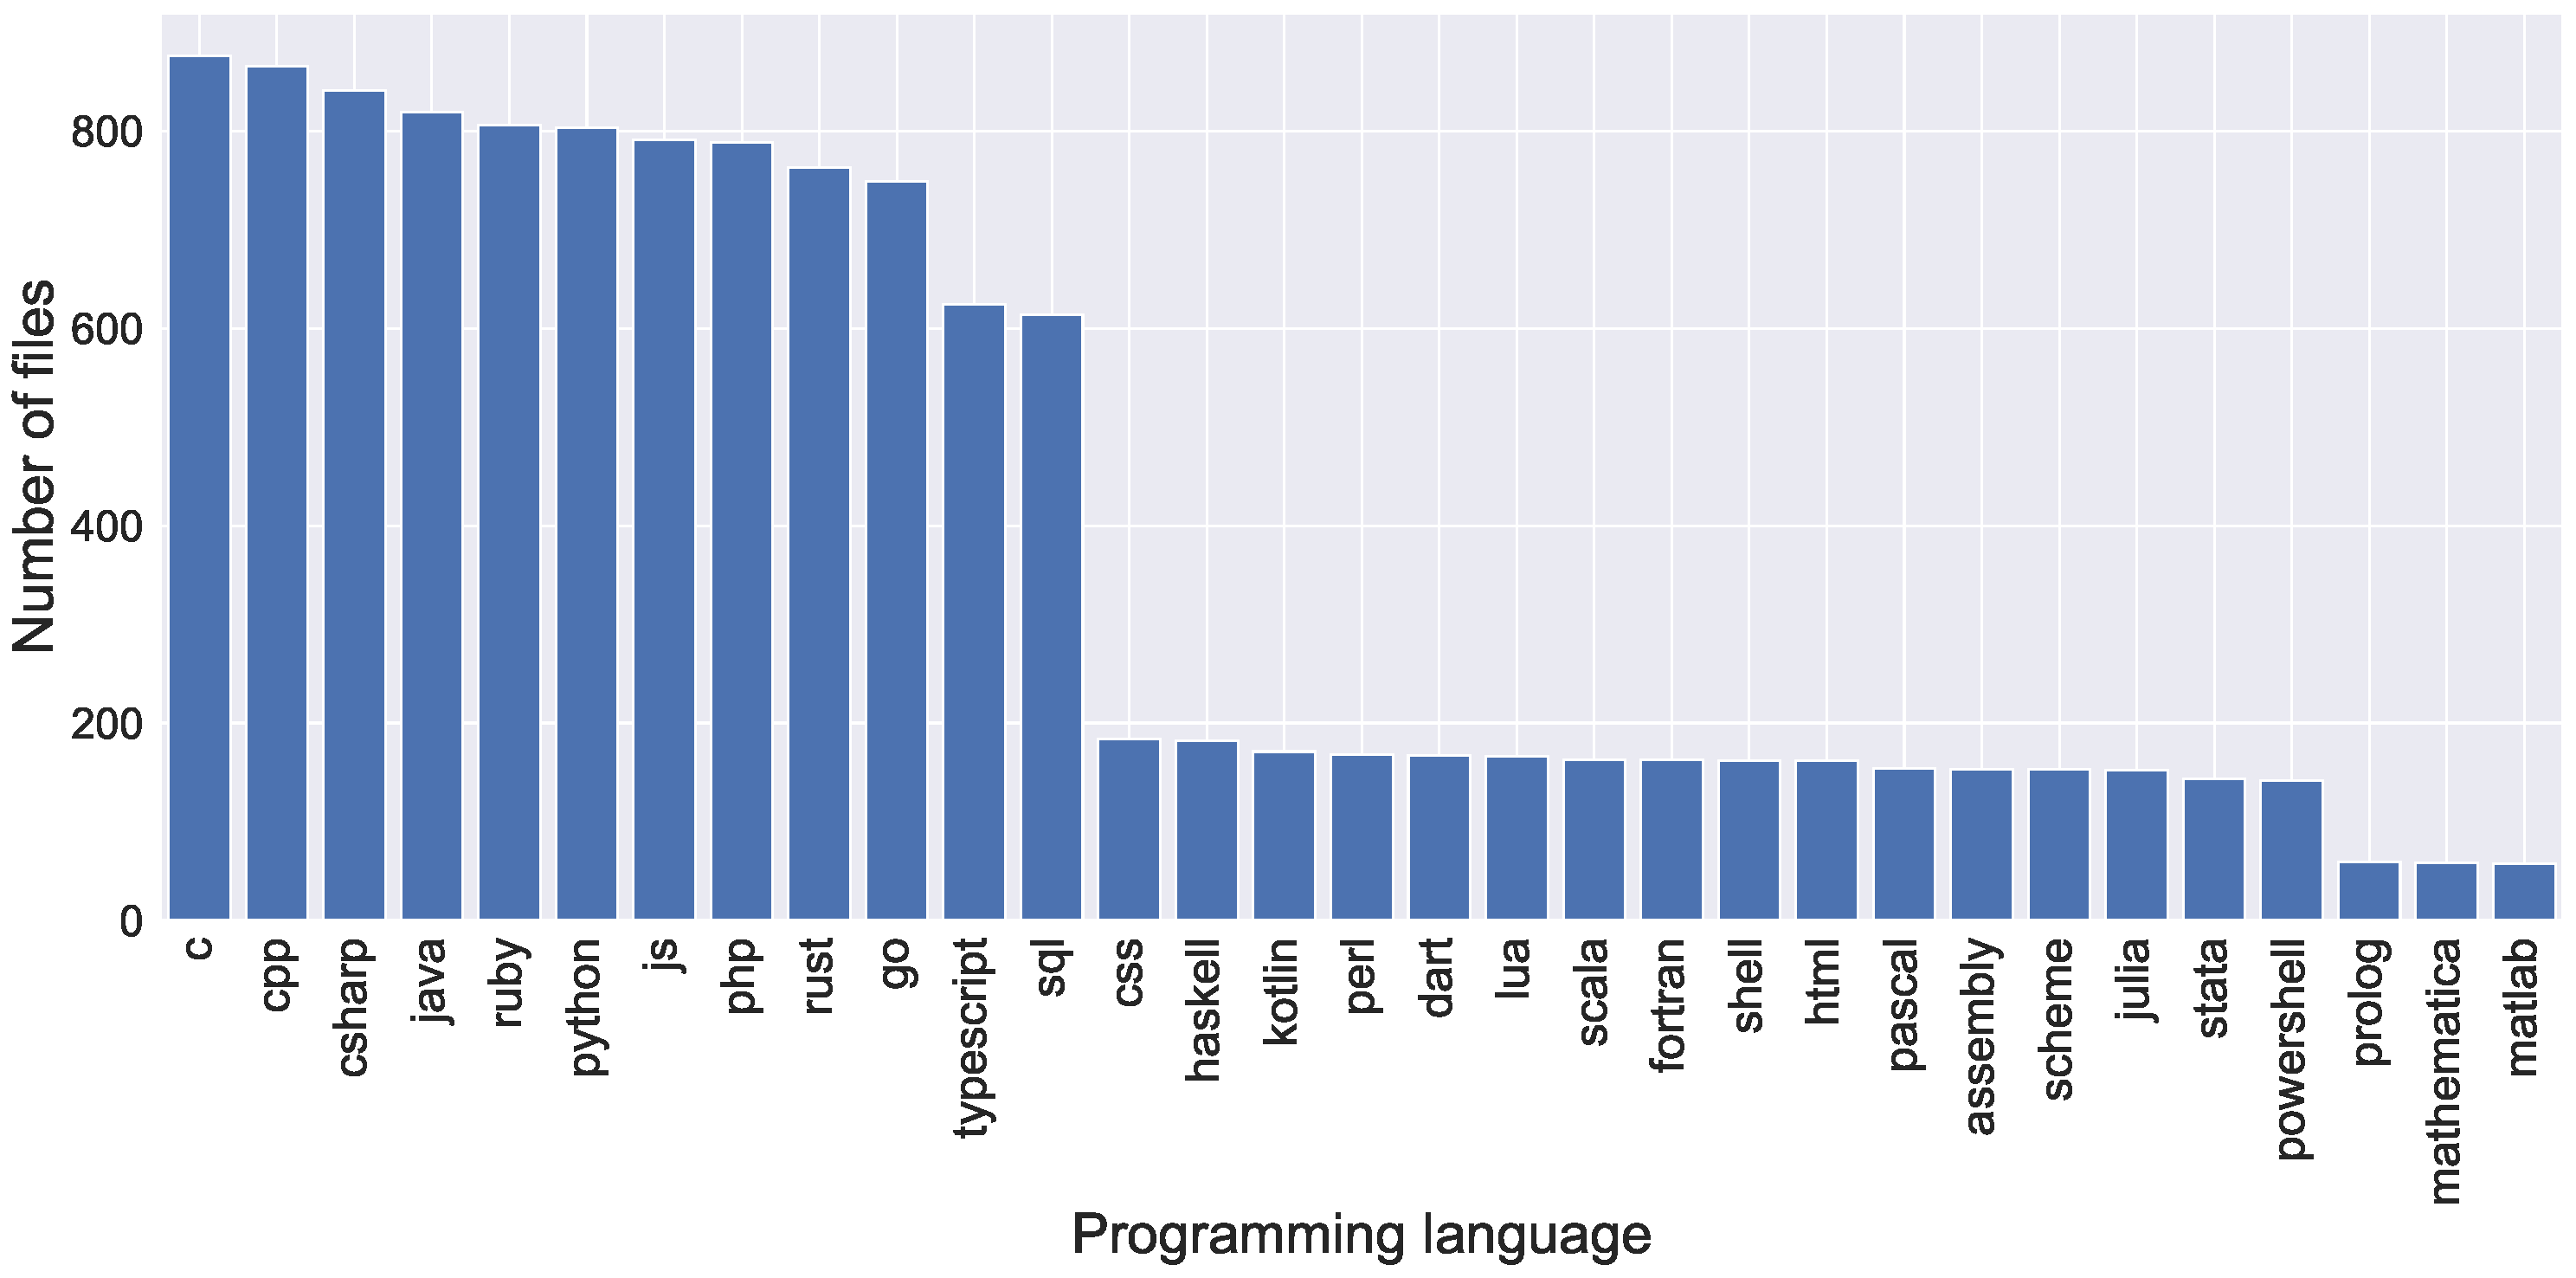
\includegraphics[scale=0.28]{figures/pii_lang_dist.pdf}
    \caption{Distribution of programming languages in the annotated PII dataset.}
    \label{fig:pii_langs}
\end{figure}

During annotation, we differentiated between various types of PII based on the specific context in which it appeared. Specifically, we distinguished whether the PII was present in the code's license header, was used as a placeholder, or constituted confidential data. This categorization was necessary because the PII in license headers is usually provided voluntarily by authors for code attribution and may not require masking. Similarly, placeholders are not real secrets and do not need to be masked. We applied this categorization to names, emails, and usernames. See Table~\ref{tab:dist_pii} for an overview of all PII entities. 

The annotators detected a total of 22,950~PII entities in the dataset. To evaluate the quality of the dataset, we manually inspected 300~files that contained various PII types and calculated the recall and precision for each type, as shown in Table~\ref{tab:dist_pii}. We found that annotating secret IDs was particularly challenging, as the annotators tended to produce many false positives and negatives. As a result, we decided to exclude this category from the PII detection model training.

\begin{table}[ht]
\centering
\begin{tabular}{lccc}
\toprule
\textbf{PII type} & \textbf{Count} & \textbf{Recall} & \textbf{Precision}\\
\midrule
IP\_ADDRESS & 2526 & 85\% & 97\% \\
KEY & 308 & 91\% & 78\% \\
PASSWORD & 598 & 91\% & 86\%\\
ID & 1702 & 53\% & 51\% \\

EMAIL & 5470 & 99\% & 97\%\\
EMAIL\_EXAMPLE & 1407 \\
EMAIL\_LICENSE & 3141 \\

NAME & 2477 & 89\% & 94\% \\
NAME\_EXAMPLE & 318 \\
NAME\_LICENSE & 3105 \\

USERNAME & 780 & 74\% & 86\% \\
USERNAME\_EXAMPLE & 328 \\
USERNAME\_LICENSE & 503 \\

AMBIGUOUS & 287 \\ \bottomrule
\end{tabular}
\caption{Overview of the PII types and the number of collected annotations. We investigate the annotation quality by reporting the precision and recall of a manual inspection on 300 files. Each subcategory was mapped back to its corresponding PII type for the inspection.}
\label{tab:dist_pii}
\end{table}


\subsection{StarEncoder}\label{sec:bigcode_encoder}
As part of our PII detection efforts, we trained an encoder-only model (i.e., bi-directionally self-attentive Transformers) that can be efficiently fine-tuned for both code- and text-related tasks. We used the Masked Language Modelling (MLM) and Next Sentence Prediction (NSP) objectives from BERT~\citep{devlin2018bert,liu2019roberta} and predicted masked-out tokens from an input sentence and whether a pair of sentences occur as neighbors in a document. 
% We refer to those two objectives as~$\mathcal{L}_{\mathit{MLM}}$ and~$\mathcal{L}_{\mathit{NSP}}$, respectively, and define the training objective $\mathcal{L}$ as their sum:

% \begin{equation}
% \mathcal{L} = \mathcal{L}_{MLM} + \mathcal{L}_{NSP}.
% \end{equation}

%Post-tokenization pre-processing operations are further performed to create training pairs. 
% Special tokens are added to separate code snippets and represent each input as follows: $$[CLS] \{\text{Snippet-1}\} [SEP] \{\text{Snippet-2}\} [SEP],$$ where two code snippets are selected randomly, and a decision is made on-the-fly as to whether the two pieces of code are neighbors from the same source file or are picked from two distinct documents. Tokens are masked out independently with a probability of 15\%, and the results define the input-output pairs used to compute $\mathcal{L}_{\mathit{MLM}}$. On the other hand, $\mathcal{L}_{\mathit{NSP}}$ is computed using a linear classifier trained on top of the representations output at the $[CLS]$ special token.

% possible alternate phrasing:
We separate code snippets in the input as follows: \texttt{[CLS]} Snippet-1 \texttt{[SEP]} Snippet-2, where the two code snippets are selected randomly, either from the same source file or from two distinct documents. For the MLM loss, we mask tokens in the input independently with an probability of 15\%. For the NSP loss, we use a linear classifier applied to the representation output at the \texttt{[CLS]} token. 
We train for 100,000~steps with a global batch size of 4,096~sequences of a maximum length of~1,024 so that approximately 400B~tokens are observed. This takes roughly two days using 64~NVIDIA A100~GPUs. Details about the model architecture are reported in Table~\ref{tab:encoder_arch}. 

% sequence-to-sequence and sequence-level prediction tasks. In addition, we would like to obtain models yielding representations that perform well when evaluated in a zero-shot fashion for information retrieval tasks, such as code search from either text or even from code in a different programming language. To achieve that, we employed a multi-task training scheme where two groups of objectives are minimized simultaneously. To ensure good token-level representations were learned, we leveraged the training objectives from BERT~\citep{devlin2018bert,liu2019roberta}. That is, the model is trained to predict masked-out tokens from an input sentence and to predict whether a pair of sentences occur as neighbors in a document. We refer to those two objectives as~$\mathcal{L}_{\mathit{MLM}}$ and~$\mathcal{L}_{\mathit{NSP}}$, respectively.

% In addition, useful sequence-level representations are enforced via a contrastive objective~$\mathcal{L}_{CONT}$, similar to SimCSE~\citep{gao2021simcse}, where sentence embeddings are forced to match for positive pairs, given by independently transformed versions of a given data instance. In this case, input transformations correspond to randomly dropping out tokens. In summary, our overall  training objective~$\mathcal{L}$ is given by the following:

% \begin{equation}
% 	\mathcal{L} = \alpha (\mathcal{L}_{MLM} + \mathcal{L}_{NSP}) + (1-\alpha) \mathcal{L}_{CONT},
% \end{equation}
% where the hyperparameter $\alpha \in [0,1]$ weighs the importance of each group of objectives.

% We highlight that computing~$\mathcal{L}_{CONT}$ requires a pooling operation to be performed on top of token-level representations output by our models. We thus perform such an operation by assigning to the output at the end of sequence token the role of a global representation of the input sequence. Moreover, we implement~$\mathcal{L}_{CONT}$ following the approach in CLIP~\cite{radford2021learning}, where pairwise inner products between sequence representations are treated as parameters of a categorical distribution, and a maximum-likelihood objective is defined by assigning ground-truth targets to positive pairs.




\begin{table}[t]
\centering
\begin{tabular}{ll}
\toprule
\textbf{Hyperparameter} & \textbf{Value}\\
\midrule
Hidden size              & 768             \\
Intermediate size        & 3072            \\
Max. position embeddings & 1024            \\
Num. of attention heads  & 12              \\
Num. of hidden layers    & 12              \\ 
Attention & Multi-head\\
\midrule
Num. of parameters      & $\approx$125M \\ \bottomrule
\end{tabular}
\caption{Model architecture of StarEncoder.}\label{tab:encoder_arch}
\end{table}

\subsection{PII detection model}\label{sec:pii_model}
We fine-tuned StarEncoder on the annotated PII dataset for the Named Entity Recognition~(NER) task. We added a linear layer as a token classification head on top of the model, with 6~target classes: names, emails, keys, passwords, IP addresses, and usernames.  We excluded IDs due to low annotation quality and did not differentiate between the categorization of PII entities (license headers, placeholders) because of the model's poor performance in distinguishing them. We split the dataset into a training set of 7,878 examples and a test set of 4,000 examples, ensuring that both splits have a balanced representation of the different PII types. See Table~\ref{tab:pii_split}. We make the training and evaluation splits available under gated access at \url{https://hf.co/BigCode}.

\begin{table}
\centering
\begin{tabular}{lcc}
\toprule
\textbf{Entity type} & \textbf{Train} & \textbf{Test} \\

\midrule
EMAIL & 4721 & 1742 \\
NAME & 3847 & 1298 \\
IP\_ADDRESS & 1941 & 521 \\
USERNAME & 1320 & 346 \\
PASSWORD & 390 & 148 \\
KEY & 171 & 118 \\
\midrule
\end{tabular}
\caption{Train-test split of the annotated PII dataset.}
\label{tab:pii_split}
\end{table}

\paragraph{Fine-tuning baseline} We fine-tune StarEncoder on the PII training set, and 400 annotated files from ~\citet{allal2023santacoder}. We achieve F1 scores of more than 90\% on names, emails, and IP addresses and 73.39\%~on passwords. The model's performance is comparatively low on keys and usernames, with F1 scores of only~56.66\% and 59.39\%, respectively. We attribute the low performance on keys to the limited number of labels for this type of PII, as only 308~instances were available. For usernames, we observed the model often confused them with decorators and values in paths. This is most likely because we annotated usernames inside links for social media platforms. 

% Note: we release the final annotated dataset, for training we fine-tuned on the annotated dataset combined with a dataset from ~\citet{allal2023santacoder} containing 400 files. 

\paragraph{Pseudo-labels} To improve the detection of key and password entities, we employed a pseudo-labeling technique as described by~\citet{lee2013pseudo}. This method involves training a model on a small set of labeled data and subsequently generating predictions for a larger set of unlabeled data. Specifically, we annotated 18,000~files using an ensemble of two encoder models, which were fine-tuned on the 400-file PII dataset from \citet{allal2023santacoder}.
%\footnote{\url{https://hf.co/bigcode/deberta-v3-large-pii-ner}, \url{https://hf.co/StanfordAIMI/stanford-deidentifier-base}}
To identify reliable pseudo-labels, we calculated the average probability logits from our models and applied filtering criteria. Specifically, we set a minimum threshold of 0.5 for all entities, except for names and usernames, for which we used a higher threshold of 0.6. However, upon reviewing the results, we found a significant number of false positives for keys and passwords. As a result, we decided to only retain entities that were preceded by a trigger word, such as \texttt{key}, \texttt{auth}, or \texttt{pwd}, within the preceding 100 characters. Training on this synthetic dataset before fine-tuning on the annotated one yielded superior results for all PII categories, as demonstrated in Tables~\ref{tab:ner_regex_metrics} and \ref{tab:ner_metrics}. Only the performance for detecting usernames did not show significant improvement, so we decided to exclude it from the PII redaction process. 

\paragraph{Comparison against regex baseline} We compared our PII detection models against the regular expressions (regexes) employed in~\citet{allal2023santacoder}. The regexes only support the detection of emails, IP addresses, and keys. Note that we enhanced the email regex, as explained in the Appendix, to address false positives we found during the evaluation on this benchmark. This modification boosted the F1 score of the regex from 81.8\% to 96.83\%. Nevertheless, our PII detection models still surpassed the regex approach in detecting all three entities, as shown in Table~\ref{tab:ner_regex_metrics}. We note that the performance difference was especially large on keys and found that the \texttt{detect-secrets} tool generated many false positives, especially in specific programming languages like Go and C-sharp that weren't well represented in the regex evaluation. Consequently, the overall precision of the tool was below~4\%.

% It is worth stressing that our evaluation of the PII detection model was conducted exclusively on samples from the human-annotated dataset.

\begin{table}[t]
    \centering
    \small
    \setlength{\tabcolsep}{3.8pt} % Adjust the column separation
    \resizebox{\linewidth}{!}{
    \begin{tabular}{@{\extracolsep{3pt}}lrrr rrr rrr@{}}
        \toprule
        \multirow{2}{*}{\textbf{Method}}  & \multicolumn{3}{c}{\textbf{Email address}} & \multicolumn{3}{c}{\textbf{IP address}} & \multicolumn{3}{c}{\textbf{Key}} \\ \cmidrule{2-4}\cmidrule{5-7}\cmidrule{8-10}
         & \textbf{Prec.} & \textbf{Recall} & \textbf{F1} & \textbf{Prec.} & \textbf{Recall} & \textbf{F1}  & \textbf{Prec.} & \textbf{Recall} & \textbf{F1} \\
        \midrule
        Regex &  96.20\% & 97.47\% & 96.83\% & 71.29\% & 87.71\% & 78.65\% & 3.62\% & 49.15\% & 6.74\% \\
        NER & 94.01\% & 98.10\% & 96.01\% & 88.95\% &\textbf{ 94.43\%} & 91.61\% & 60.37\% & 53.38\% & 56.66\%  \\
        + pseudo labels &  \textbf{97.73\%} & \textbf{98.94\% }& \textbf{98.15\% }& \textbf{90.10\%} & 93.86\% & \textbf{91.94\%} & \textbf{62.38\%} & \textbf{80.81\%} & \textbf{70.41\%} \\
        \bottomrule
    \end{tabular}}
    \caption{Comparing PII detection performance: Regular Expressions, NER Pipeline with Annotated Data, and NER Pipeline with Annotated Data + Pseudo-Labels}
    \label{tab:ner_regex_metrics}
\end{table}

\begin{table}[t]
    \centering
    \small
    \setlength{\tabcolsep}{3.pt} % Adjust the column separation
    \resizebox{\linewidth}{!}{
        \begin{tabular}{@{\extracolsep{3pt}}lrrr rrr rrr@{}}
        \toprule
        \multirow{2}{*}{\textbf{Method}}  & \multicolumn{3}{c}{\textbf{Name}} & \multicolumn{3}{c}{\textbf{Username}} & \multicolumn{3}{c}{\textbf{Password}} \\ \cmidrule{2-4}\cmidrule{5-7}\cmidrule{8-10}
         & \textbf{Prec.} & \textbf{Recall} & \textbf{F1} & \textbf{Prec.} & \textbf{Recall} & \textbf{F1}  & \textbf{Prec.} & \textbf{Recall} & \textbf{F1} \\
        \midrule
        NER & 83.66\% & 95.52\% & 89.19\% & 48.93\% & \textbf{75.55\%} & 59.39\% & 59.16\% & \textbf{96.62\%} & 73.39\% \\
        + pseudo labels & \textbf{86.45\%} & \textbf{97.38\% }& \textbf{91.59\% }& \textbf{52.20\%} & 74.81\% & \textbf{61.49\%} & \textbf{70.94\% }& 95.96\% & \textbf{81.57\% }\\
        \bottomrule
    \end{tabular}}
    \caption{Comparison of PII detection performance: NER Pipeline with Annotated Data vs.\ Annotated Data + Pseudo-Labels}
    \label{tab:ner_metrics}
\end{table}

\paragraph{Post-processing} Before applying the best PII detection model to the full dataset, we observed a couple of frequent detection errors. We added the following post-processing techniques to reduce the number of false positives:
\begin{itemize}
    \item Ignore secrets with fewer than 4~characters.
    \item Detect full names only by requiring at least one space within the name.
    \item Ignore detected keys with fewer than 9~characters or that are not gibberish using a \texttt{gibberish-detector}.\footnote{\url{https://github.com/domanchi/gibberish-detector}}
    \item Ignore IP addresses that aren't valid or are private (non-Internet facing) using the \texttt{ipaddress} python package. We also ignore IP addresses from popular DNS servers. We use the same list as in~\cite{allal2023santacoder}.
\end{itemize}

% given that issues primarily consist of natural language text.



\paragraph{PII placeholders} We replaced the detected PII entities with the following tokens: 
\begin{verbatim}
<NAME>, <EMAIL>, <KEY>, <PASSWORD>
\end{verbatim}
To mask IP addresses, we randomly selected an IP address from 5~synthetic, private, non-internet-facing IP addresses of the same type that can be found in Appendix~\ref{sec:ipaddress_replacement}.

\paragraph{Github issues} We already employed a regex approach to detect keys, IP addresses, and emails in the Github issues, so we only used the PII detection model to redact names. We anonymized the usernames of the authors by replacing them with a participant counter within the conversation,  e.g. username\_1 to refer to second participant (see Section \ref{sec:data_formatting} for formatting details). We prepend these pseudonyms to the beginning of each comment such that we preserve the speaker identity of the author. In addition, we redact all mentions of these usernames in the messages. Note that we only mask the usernames of active participants in the conversation and mentions of non-participating users are not anonymized. 

\paragraph{Compute resources} We used the PII detection model to identify PII across all programming languages in the training dataset, including GitHub issues (names only), Git commits, and Jupyter notebooks. The total dataset amounts to 815~GB in size. We ran inference on multiple NVIDIA~A100 80~GB~GPUs, which required 800~GPU-hours. 

\section{Model training}\label{sec:model_training}
This section presents information on the training process of the StarCoder models. Before we proceed, we first clarify the differences between the two models:

\begin{description}
\item[StarCoderBase] is the first model trained on 1 trillion tokens sourced from the curated dataset described in Section \ref{sec:data_curation}. 

\item[StarCoder] is the fine-tuned version of StarCoderBase, trained on another 35B Python tokens (roughly 2 epochs).  
\end{description}

Throughout the following, we show how we formatted the training data (Section~\ref{sec:data_formatting}), decontaminated the training data (Section~\ref{sec:decontamination}), and provide details regarding the tokenizer (Section~\ref{sec:tokenizer}), the model architecture (Section~\ref{sec:model_architecture}), the training process (Section~\ref{sec:training_details}),  multi-node GPU setup (Section~\ref{sec:multinode_training}), and CO2 emissions (Section~\ref{sec:co2emission}). 

\subsection{Data formatting}\label{sec:data_formatting}
We present the formatting guidelines for each of the data sources below. We provide the templates below in which <token> refers to a sentinel token, and \textcolor{red}{metadata} and \textcolor{blue}{data} refer to placeholders for data fields, respectively. 

\paragraph{Code} We prepend the repository name, file name, and the number of stars to the context of the code file. To not overfit on the exact number of stars, we categorized GitHub stars into five buckets: 0, 1--10, 10--100, 100--1000, 1000+. To enable the model to operate without this metadata during inference, we prefixed the repository name, filename, and stars independently at random, each with a probability of~$0.2$. 

\begin{Verbatim}[commandchars=!\{\}]
<reponame>!textcolor{red}{reponame}<filename>!textcolor{red}{filename}<gh_stars>!textcolor{red}{stars}\n!textcolor{blue}{code}<|endoftext|>
\end{Verbatim}

To the source code in this template (i.e. \textcolor{blue}{code}), we apply the \textbf{fill-in-the-middle transformation}~\citep[FIM;][]{bavarian2022fim}. More precisely, we apply FIM at the character-level to the source code files with a FIM-rate of 0.5, and use PSM mode with probability .5 and SPMv2 mode with probability .5. 

\paragraph{Issues} We use sentinel tokens to mark the opening of an issue and subsequently include its title. We separate the sequence of comments by a <issue\_comment> token and include a anonymized speaker identifier before the comment. Specifically, we refer to authors by their participant counter within the conversation, e.g.  username\_1 to refer to second participant in the issue. To distinguish between the different turns, we use \textcolor{blue}{comment1}, \textcolor{red}{id1} to refer to the second comment and its anonymized speaker id, respectively. 

\begin{Verbatim}[commandchars=!\{\}]
<issue_start>Title: !textcolor{blue}{title}\nusername_!textcolor{red}{id0}:!textcolor{blue}{comment0}<issue_comment>username_!textcolor{red}{id1}:!textcolor{blue}{comment1}
... <issue_closed (optional)><|endoftext|>
\end{Verbatim}


\paragraph{Jupyter -- scripts}

Jupyter scripts were formatted in the same manner as code.

\paragraph{Jupyter -- structured} Parsed Jupyter notebooks come in chains of text, code, and outputs, and we separated them with sentinel tokens. Note that we use \textcolor{blue}{text2}, \textcolor{blue}{code2}, \textcolor{blue}{output2} to refer to the 3rd triplet in the notebook.  

\begin{Verbatim}[commandchars=!\{\}]
<jupyter_start><jupyter_text>!textcolor{blue}{text0}<jupyter_code>!textcolor{blue}{code0}
<jupyter_output>!textcolor{blue}{output0}<jupyter_text> ... <|endoftext|> 
\end{Verbatim}



\paragraph{Git commits} We separate the code before the commit, the commit message, and the code after the commit with sentinel tokens. As explained in Section~\ref{sec:commits}, we use the full files with 20\% probability and otherwise use a small window (0-32 lines) around the changed lines. 

\begin{Verbatim}[commandchars=!\{\}]
<commit_before>!textcolor{blue}{code_before}<commit_msg>!textcolor{blue}{message}<commit_after>!textcolor{blue}{code_after}<|endoftext|>
\end{Verbatim}
%As we found the structure of diffs is more complex, we predict the full code with changes rather than diffs.

We summarize all sentinel tokens in Table~\ref{tab:sentinel_tokens}. 

\begin{table}[t]
\centering
\begin{tabular}{ll}
\toprule
\textbf{Token} & \textbf{Description}\\
\midrule
 \verb$<|endoftext|>$ & end of text/sequence \\ 
 \verb|<fim_prefix>| & FIM prefix  \\  
 \verb|<fim_middle>| & FIM middle \\
 \verb|<fim_suffix>| & FIM suffix \\
 \verb|<fim_pad>| & FIM pad \\
 \verb|<reponame>| & repository name \\
 \verb|<filename>| & file name  \\
 \verb|<gh_stars>| & GitHub stars\\
 \verb|<issue_start>| & start of GitHub issue \\
 \verb|<issue_comment>| & start of GitHub issue comment \\
 \verb|<issue_closed>| & GitHub issue closed event \\
 \verb|<jupyter_start>| & start of Jupyter notebook \\
 \verb|<jupyter_text>| & start of Jupyter text cell \\
 \verb|<jupyter_code>| & start of Jupyter code cell \\
 \verb|<jupyter_output>| & start of Jupyter output cell \\
 \verb|<empty_output>| & output cell without content \\
 \verb|<commit_before>| & code snippet before commit\\
 \verb|<commit_msg>| & commit message \\
 \verb|<commit_after>| & code snippet after commit\\
\bottomrule
\end{tabular}
\caption{Overview of the sentinel tokens. }\label{tab:sentinel_tokens}
\end{table}

\subsection{Training data decontamination}\label{sec:decontamination}

The code training data was decontaminated by removing files that contained 
%test samples from the following benchmarks: HumanEval (and hence MultiPL-E), MBPP, APPS, GSM8K, and DS1000.
docstrings or solutions from HumanEval and MBPP, docstrings from APPS, questions from GSM8K, or prompts from DS1000. (These benchmarks are further described in Section~\ref{sec:evaluation}.)
To give an indication of the amount of data removed by decontamination, Python is the language with the highest number of matches, with 558~files removed.

\subsection{Tokenizer}\label{sec:tokenizer}
The model's tokenizer follows our insights presented in \citet{allal2023santacoder} and uses those same design choices: we use the Hugging Face Tokenizers library~\citep{anthony_moi_2022_hftokenizers} to train a byte-level Byte-Pair-Encoding with a vocabulary size of 49,152 tokens---including the sentinel tokens from table~\ref{tab:sentinel_tokens}. The pre-tokenization step includes a digit-splitter and the regex splitter from the GPT-2 pre-tokenizer.

\subsection{Model Architecture}\label{sec:model_architecture}
We trained a 15.5B parameter model with the same architecture as SantaCoder~\citep{allal2023santacoder}. It is a decoder-only Transformer with Multi-Query-Attention~\citep[MQA;][]{shazeer2019mqa}, and learned absolute positional embeddings. We also apply Fill-in-the-Middle~\citep[FIM;][]{bavarian2022fim} transformations to the training data, see Section \ref{sec:data_formatting}. We used FlashAttention~\citep{dao2022flashattention} to speed up the attention computation and reduce its memory footprint, allowing us to scale to a 8K context length. To make FlashAttention work with MQA during training, we simply expand the key and value before calling the attention kernel. The architecture hyper-parameters are given in Table~\ref{tab:decoder_arch}.  In addition, we have included the hyperparameters of SantaCoder\citep{allal2023santacoder} for comparison.  

\subsection{Training details}\label{sec:training_details}
\paragraph{StarCoderBase} The model was trained for 250k~iterations, with a batch size of 4M~tokens, for a total of one trillion tokens.  We used Adam~\citep{DBLP:journals/corr/KingmaB14} with~$\beta_1=0.9$, $\beta_2=0.95$, $\epsilon=10^{-8}$ and a weight decay of~$0.1$. The learning rate followed a cosine decay from~$3\times10^{-4}$ to~$3\times10^{-5}$ after a linear warmup of 2,000~iterations.

\paragraph{StarCoder} Starting from StarCoderBase, we fine-tuned a Python variant of the model for 2 epochs on the Python subset of the training data.  We used the same settings as StarCoderBase, except that we used a learning rate of ~$5\times10^{-5}$ and decayed it to~$5\times10^{-6}$ after 1,000~iterations of linear warmup. We trained for 8,500~steps. 

\begin{table}[t]
\centering
\begin{tabular}{lll}
\toprule
\textbf{Hyperparameter} & \textbf{SantaCoder} &\textbf{StarCoder}\\
\midrule
Hidden size              & 2048 & 6144             \\
Intermediate size        & 8192 & 24576            \\
Max.\ position embeddings & 2048 & 8192            \\
Num.\ of attention heads  & 16 &  48              \\
Num.\ of hidden layers    & 24 &  40              \\ 
Attention & Multi-query &  Multi-query\\
\midrule
Num.\ of parameters      & $\approx$ 1.1B & $\approx$15.5B \\ 
\bottomrule
\end{tabular}
\caption{Model architecture of StarCoder. We also include SantaCoder (prior work by the community). }
\label{tab:decoder_arch}
\end{table}


% Table with hyperparameters

\subsection{Multi-Node GPU Setup}\label{sec:multinode_training}

We trained our model on a GPU cluster with 512~A100 80~GB~GPUs distributed across 64~nodes. We partitioned the model with a 3D-parallel layout that shards the model with both tensor and pipeline parallelism rank~4, requiring 16~GPUs (two nodes) for one replica. To fully leverage the cluster's capabilities, we used 32-fold data parallelism. To optimize GPU utilization and reduce idle compute bubbles, we maintained a micro-batch size of~1 and accumulated for 16~steps, resulting in a global batch size of~512 (equivalent to 4M~tokens). We used Megatron-LM's distributed optimizer because we found that it leads to slightly higher throughput in this configuration. Since it requires the gradient reduction step in FP32, the training in BF16 leads to 10\%~lower throughput than~FP16, but we used it anyway to avoid training instabilities.  

Except for a few restarts, we did not experience significant training instabilities. 

\subsection{CO2 emissions}\label{sec:co2emission}
\paragraph{StarCoderBase} We report the carbon footprint~\citep{lacoste2019quantifying} of training StarCoderBase. Based on the total number of GPU hours that training took (320,256) and an average power usage of 280W per GPU, this adds up to 89671.68 kWh of electricity consumed during the training process. Multiplied by the carbon intensity of the energy of the us-west-2 AWS location (0.15495 kgCO2e per kWh) and the average Power Usage Effectiveness of 1.2 across AWS datacenters,  this results in 16.68 tonnes of CO2eq emitted. 

\paragraph{StarCoder} The fine-tuned model adds 3.5\% of training time, which translates to an additional estimated emission of 0.58 tonnes of CO2eq.  \
% you can add this link as a reference for carbon intensity: https://www.carbonfootprint.com/docs/2022_03_emissions_factors_sources_for_2021_electricity_v11.pdf

\section{Evaluation}\label{sec:evaluation}

In this section, we first outline the models we evaluated in addition to StarCoder and StarCoderBase. Then we report on the Python language performance of all models on the HumanEval~\citep{chen2021codex}, MBPP~\citep{austin2021program}, and DS-1000~\citep{Lai2022DS1000} evaluation benchmarks. Then we cover multi-language evaluation using a variety of benchmarks and tasks.

\paragraph{A Code LM Evaluation Harness}

To enable reproducible and centralized evaluation of StarCoder and other Code LLMs, we developed a Code LM Evaluation Harness~\citep{bigcode-evaluation-harness}, inspired by the LM Evaluation-Harness~\citep{eval-harness}. This harness provides a framework for the efficient evaluation of code models, utilizing data parallelism and docker containers for execution. It supports several benchmarks, including HumanEval, MultiPL-E, and DS-1000.

\paragraph{Other Models Evaluated} We compare StarCoder and StarCoderBase to the following models.

\begin{enumerate}
\item \textbf{CodeGen-16B-Multi}~\citep{nijkamp:codegen} is an open-access, 16B~parameter model that is trained on the Pile~\citep{gao2020pile}, and then
on additional code written in C, \cpp{}, Go, Java, JavaScript, and Python from the GitHub BigQuery dataset~\citep{smith2016bigquery}.

\item \textbf{CodeGen-16B-Mono} is a version of CodeGen-16B-Multi that is fine-tuned on additional Python code from GitHub, though the dataset is not publicly available.

\item \textbf{CodeGeeX}~\citep{qinkai:codegeex} is an open-access 13B~parameter model trained on 23~programming languages selected from the Pile, the CodeParrot dataset~\citep{wolf-etal-2020-transformers}, and additional data for Python, Java, and \cpp{}. CodeGeeX also includes its own multi-language benchmark suite, HumanEval-X, which we discuss below. 

\item \textbf{code-cushman-001} is a 12B~parameter model by OpenAI and was the initial model for GitHub Copilot~\citep{chen2021codex}. The details of its training set are unknown. This model has been deprecated by OpenAI but was available from the Microsoft Azure OpenAI Service at the time of writing.\footnote{There had been a code-cushman-002, but it is not available at the time of writing.}

\item Finally, although they are not specifically trained for code generation, we include some results from the LLaMA~\citep{touvron2023llama}, PaLM~\citep{chowdhery2022palm}, and LaMDA~\citep{thoppilan2022lamda} papers. LLaMA's license prohibits commercial use, and PaLM and LaMDA are not publicly available.

\end{enumerate}

\subsection{StarCoder: Python Evaluation}

In this section, we evaluate the performance of StarCoder on Python, comparing it to both open-access and closed-access models. We first report performance on HumanEval~\citep{chen2021codex} and MBPP~\citep{austin2021program}, which are two widely used benchmarks of Python performance. However, we also measure performance on DS-1000~\citep{Lai2022DS1000}, a code completion benchmark of 1,000 Python data science problems based on StackOverflow questions.


\begin{table}[t]
\centering
% ARJUN DO NOT PASTE ANYTHING HERE, MANUALLY EDIT"
% \begin{tabular}{lcc}
% \toprule
% \textbf{Model} &  \textbf{HumanEval} &  \textbf{MBPP} \\
%              % &            &        \\
% \midrule
% LLaMA-7B          &      10.5 &  17.7 \\
% LaMDA-137B        &      14.0 &  14.8 \\
% LLaMA-13B         &      15.8 &  22.0 \\
% CodeGen-16B-Multi &      18.3 &  20.9 \\
% LLaMA-33B         &      21.7 &  30.2 \\
% CodeGeeX          &      22.9 &  24.4 \\
% LLaMA-65B         &      23.7 &  37.7 \\
% PaLM-540B         &      26.2 &  36.8 \\
% CodeGen-16B-Mono  &      29.3 &  35.3 \\
% StarCoderBase     &      30.4 &  49.0 \\
% code-cushman-001  &      33.5 &  45.9 \\
% StarCoder         &      33.6 &  \textbf{52.7} \\
% % StarCoder-Prompted & \textbf{40.8} & 49.5 \\
% \bottomrule
% % dfried: I changed to one decimal point as many of these results are from Touvron et al, which only has one (don't add zeros)
% \end{tabular}

\begin{tabular}{lrcc}
\toprule
\textbf{Model} & \textbf{Size} & \textbf{HumanEval} &  \textbf{MBPP} \\
             % &            &        \\
\midrule
\emph{Open-access} \\
LLaMA             & 7B &       10.5 &  17.7 \\
LLaMA             & 13B &      15.8 &  22.0 \\
SantaCoder        & 1.1B &     18.0 & 35.0 \\
CodeGen-Multi     & 16B &      18.3 &  20.9 \\
LLaMA             & 33B &      21.7 &  30.2 \\
CodeGeeX          & 13B &      22.9 &  24.4 \\
LLaMA-65B         & 65B &      23.7 &  37.7 \\
CodeGen-Mono      & 16B &      29.3 &  35.3 \\
StarCoderBase     & 15.5B &      30.4 &  49.0 \\
StarCoder         & 15.5B &      33.6 &  52.7 \\
% StarCoder-Prompted & 40.8 & 49.5 \\
\midrule
\emph{Closed-access} \\
LaMDA             & 137B &     14.0 &  14.8 \\
PaLM              & 540B &     26.2 &  36.8 \\
code-cushman-001  & 12B &      33.5 &  45.9 \\
code-davinci-002  & 175B &     45.9 &  60.3 \\
\bottomrule
% dfried: I changed to one decimal point as many of these results are from Touvron et al, which only has one (don't add zeros)
\end{tabular}
\caption{Comparing StarCoder's performance (pass@1) on the HumanEval and MBPP Python with several other models. StarCoder and StarCoder base obtain the highest performance of open-access models, and comparable performance to the code-cushman-001 closed access model. %obtains the including models that are not publicly available (e.g., PaLM and LaMDA).
} %Results for LLaMA, LaMDA, and PaLM are from \citet{touvron2023llama}. Results for CodeGeeX are from~\cite{qinkai:codegeex}. Results

\label{tab:pyeval}
\end{table}

\subsubsection{The HumanEval and MBPP Benchmarks}

HumanEval~\citep{chen2021codex}, and MBPP~\citep{austin2021program} are widely-used benchmarks for Code LLMs consisting of hundreds of Python programming problems that use test cases to validate the code produced by a Code LLM.
Code LLMs generate code by sampling from their output distribution. We report performance using the pass@$k$ metric~\citep{chen2021codex}: the total fraction of benchmark problems solved, where a problem is considered solved if any one of $k$ code samples passes every test case. Like \citet{chen2021codex}, we use sampling temperature~$0.2$ for pass@1, and temperature~$0.8$ for~$k > 1$. We generate $n=200$~samples for all experiments with open-access models. For API models, we use $n=20$~samples, which is enough to estimate pass@1. We focus on the simplest version of pass@$k$, which is pass@1: the likelihood that a problem is solved in a single attempt by the model.

Table~\ref{tab:pyeval} compares StarCoder (and StarCoderBase) on HumanEval and MBPP to several open-access and closed-access models:

\begin{enumerate}

  \item \emph{StarCoder is the highest-performing open-access model on both benchmarks}.
   \item \emph{StarCoder outperforms the largest models}, including PaLM, LaMDA, and LLaMA, despite being significantly smaller.

   \item \emph{StarCoderBase is also very capable on Python} and is competitive with CodeGen-16B-Mono, a similarly-sized open-access model that was fine-tuned on Python. 

   \item \emph{StarCoder outperforms OpenAI's code-cushman-001 (12B) model}.

   % \item \emph{StarCoder achieves a state-of-the-art 40\% pass@1 on HumanEval} with a simple prompt that addresses incomplete results, as described below.

\end{enumerate}

% dfried: moving this to the qualitative example section
% \paragraph{Addressing Model Failures and Prompting}

% We inspected StarCoder-generated programs on these benchmarks and found that there were several cases where the model produces what are effectively empty solutions, e.g., \texttt{pass} or a comment \emph{Insert code here}. We also observed this kind of failure in every model we evaluated. When this type of problem occurs in practice in an IDE, a programmer addresses them by altering their prompt in some ad hoc way.

% We tried a few prompt prefixes that could be applied uniformly to all benchmark problems. However, these prefixes are typically model-specific. StarCoder's input format allows us to prompt it with the name of a file using the \texttt{<filename>} token. We found that the following prefix at temperature 0.1 boosts performance on HumanEval to 40.82\%:
% \begin{verbatim}
% <filename>solutions/solution_1.py
% # Here is the correct implementation of the code exercise
% \end{verbatim}
% We also evaluated CodeGen-16B-Mono with the same temperature and prompt (but had to omit the filename since the CodeGen models do not support them). But, we found that this hurts performance, bringing it down to 
% 28.10\%. However, some other prefixes may exist that improve its performance. Similarly, we found that this prompt had a negligible impact with StarCoderBase.

\subsubsection{The DS-1000 Python Data Science Benchmarks}

\begin{table}[t]
\centering
\resizebox{\linewidth}{!}{
\begin{tabular}{llcccccccc}
\toprule
\textbf{Format} & \textbf{Model} & \textbf{\rotatebox{35}{\parbox{1.2cm}{\small Matplotlib}}} & \textbf{\rotatebox{35}{\parbox{1.2cm}{\small NumPy}}} & \textbf{\rotatebox{35}{\parbox{1.2cm}{\small Pandas}}} & \textbf{\rotatebox{35}{\parbox{1.2cm}{\small PyTorch}}} & \textbf{\rotatebox{35}{\parbox{1.2cm}{\small SciPy}}} & \textbf{\rotatebox{35}{\parbox{1.2cm}{\small Scikit-Learn}}} & \textbf{\rotatebox{35}{\parbox{1.2cm}{\small TensorFlow}}} & \textbf{Overall} \\

\midrule
           & \textrm{Number of problems:} 
& 155 & 220 & 291 & 68 & 106 & 115 & 45 & 1,000\\
\midrule
Completion & SantaCoder-1B & 21.6 & 4.6 & 0.9 & 2.6 & 2.4 & 4.8 & 3.1 & 5.7\\ 
Completion & InCoder-6B & 28.3 &  4.4 & 3.1 & 4.4 &  2.8 & 2.8 & 3.8 & 7.4 \\ 
Completion & CodeGen-16B-Mono & 31.7 & 10.9 & 3.4 & 7.0 & 9.0 & 10.8 & 15.2 & 11.7 \\ 
Completion & code-cushman-001 & 40.7 & 21.8 & 7.9 & 12.4 & 11.3 & 18.0 & 12.2 & 18.1 \\ 
Completion & StarCoderBase & 47.0 & 27.1 & 10.1 & 19.5 & \textbf{21.7} & 27.0 & 20.5 & 23.8 \\ 
Completion & StarCoder & \textbf{51.7} & \textbf{29.7} & \textbf{11.4} & \textbf{21.4} & 20.2 & \textbf{29.5} & \textbf{24.5} & \textbf{26.0} \\
%Completion & code-davinci-001 & 41.8 & 26.6 & 9.4 & 9.7 & 15.0 & 18.5 & 17.2 & 20.2 \\ 
%Completion & code-davinci-002 & 57.0 & 43.1 & 26.5 & 41.8 & 31.8 & 44.8 & 39.3 & 39.2 \\ 
\midrule
Insertion & SantaCoder-1B & 21.6$^*$ & 13.8 & 2.0 & 3.8 & 5.7 & 6.9 & 14.8 &  9.3 \\ 
Insertion & InCoder-6B & 28.3$^*$ & 4.6 & 2.9 & 4.4 & 2.8 & 3.1 & 7.8 & 7.5 \\ 
Insertion & StarCoderBase & 47.0$^*$ & 26.3 & \textbf{10.9} & 16.6 & \textbf{20.2} & \textbf{30.2} & \textbf{22.3} & 24.0 \\ 
Insertion & StarCoder & \textbf{51.7}* & \textbf{30.8} & 10.3 & \textbf{21.0} & \textbf{20.2} & 27.4 & 20.0 & \textbf{25.4} \\
%Insertion & code-davinci-002 & 57.0* & 46.5 & 30.1 & 47.7 & 34.8 & 53.7 & 53.4 & 43.3 \\ 
\bottomrule
\end{tabular}
}
\caption{Performance of open-access and closed-access models on DS-1000. Benchmarks are as follows. All models evaluated at temperature=0.2, top\_p=0.5, max\_length=1024. Scores reflect mean pass@1 accuracy averaged over 40 samples. $^*$: Matplotlib task does not have right sided context, so insertion and completion formats are identical.} 
\label{tab:ds1000}
\end{table}

A major limitation of HumanEval and MBPP is that they are simple programming puzzles that are not representative of the code that most programmers write. In contrast, the DS-1000 benchmark~\citep{Lai2022DS1000} has a suite of 1,000 realistic and practical data science workflows across seven libraries and evaluates generations in execution against test cases.

DS-1000 supports two evaluation modes: completion and insertion (via FIM). We report completion scores for all models but insertion scores only for models that support it: the StarCoder models and InCoder-6B~\citep{fried2022incoder}.
DS-1000 also categorizes problems based on the libraries used: Matplotlib, NumPy, Pandas, SciPy, Scikit-Learn, PyTorch, and TensorFlow.  We report pass@1 for each library and an overall score in
Table~\ref{tab:ds1000} and draw the following conclusions:

\begin{enumerate}

  \item \emph{StarCoder substantially outperforms all other models on data science problems} from the DS-1000 benchmark. Moreover, this is true across every kind of data science library.

  \item \emph{StarCoderBase also outperforms every other model}, but is slightly behind StarCoder on DS-1000.

  \item We confirm the finding by \citet{Lai2022DS1000}: \emph{model performance on HumanEval and MBPP benchmarks does not always correlate with performance on the more realistic DS-1000 benchmarks}. For example, CodeGen-Mono slightly outperforms code-cushman-001 and the StarCoder models on HumanEval and MBPP, but is significantly worse on DS-1000. This demonstrates the importance of evaluating models on a range of benchmarks.

\end{enumerate}

%Overall, we see that StarCoder outperforms all tested models on all benchmark subsets across completion and insertion formats of the benchmark.


\subsubsection{The ODEX Open-Domain Coding Benchmark}
Our previous evaluations focus either on \emph{closed domains} (i.e., primarily built-in Python functions, as in MBPP and HumanEval) or specific domains (e.g., data science, as in DS-1000). To evaluate model ability to generate code on a broader set of Python libraries, we use the ODEX benchmark~\citep{wang2022execution} containing 505 open-domain and 440 closed-domain Python coding queries, in four natural languages --- English, Spanish, Japanese, and Russian --- with test-case-based execution evaluation.

We report the pass@1 metric for StarCoder and baseline models, including Codex (code-davinci-001), CodeGen-16B-Mono, and SantaCoder. 
In addition to the overall execution accuracy, we also categorize problems by languages and domains, which are: (1) queries in the \emph{closed-domain} (using only built-in Python functions) and \emph{open-domain} (using functions from imported libraries), and (2) queries with instructions written in English, Spanish, Japanese, and Russian, respectively. We report overall scores and scores in different domains and languages in Table~\ref{tab:odex_language-domain} and draw the following conclusions:

\begin{enumerate}

  \item \emph{StarCoder substantially outperforms all other models on open-domain coding queries} from the ODEX benchmark. 

  \item \emph{StarCoderBase also outperforms every other model}, even better than StarCoder in the ODEX English subset, but slightly behind in other languages.

  \item Both StarCoder and StarCoderBase models generally exhibit smaller gaps between open- and closed-domain queries than other baseline models, despite the higher overall execution accuracy. This result indicates that StarCoder models acquire more generalized skills about coding queries in the open domain (i.e., concerning diverse Python libraries), while other models exhibit larger performance drops when moving from the closed to open domain.
\end{enumerate}

% \begin{table}[ht]
% \centering
% \resizebox{\linewidth}{!}{
% \begin{tabular}{l|ccc|ccc|ccc|ccc}
% \toprule
% \multirow{2}{*}{\textbf{Model}} & \multicolumn{3}{c|}{English} & \multicolumn{3}{c|}{Spanish} & \multicolumn{3}{c|}{Japanese} & \multicolumn{3}{c}{Russian} \\
% {} & {-} & {open} & {closed} & {-} & {open} & {closed} & {-} & {open} & {closed} & {-} & {open} & {closed} \\
% \midrule
% CodeGen-16B & 33.71 & 25.22 & 43.06 & 30.00 & 25.00 & \textbf{43.06} & 37.80 & 26.55 & \textbf{62.75} & 46.83 & 30.40 & 60.14 \\
% Codex davinci-001 & 33.62 & 26.91 & 41.00 & 36.89 & 31.67 & 42.86 & 31.04 & 23.72 & 47.25 & 43.21 & 28.86 & 55.07 \\
% SantaCoder & 37.65 & 30.87 & 45.12 & 32.11 & 26.04 & 39.05 & 28.11 & 23.01 & 39.41 & 36.87 & 22.98 & 48.33 \\
% StarCoderBase & \textbf{46.51} & \textbf{40.65} & 52.97 & 30.11 & 25.42 & 35.48 & 41.22 & 37.61 & 49.22 & 46.11 & 34.04 & 56.09 \\
% StarCoder & 44.67 & 37.00 & \textbf{53.11} & \textbf{37.56} & \textbf{32.92} & 42.86 & \textbf{44.21} & \textbf{39.56} & 54.51 & \textbf{50.40} & \textbf{33.77} & \textbf{64.13} \\
% \bottomrule
% \end{tabular}
% }
% \caption{Performance on the ODEX benchmark by instruction languages and code domains.} 
% \label{tab:odex_language-domain}
% \end{table}

\begin{table}[ht]
\centering
\resizebox{\linewidth}{!}{
\begin{tabular}{l|ccc|ccc|ccc|ccc}
\toprule
\multirow{2}{*}{\textbf{Model}} & \multicolumn{3}{c|}{English} & \multicolumn{3}{c|}{Spanish} & \multicolumn{3}{c|}{Japanese} & \multicolumn{3}{c}{Russian} \\
{} & {overall} & {open} & {closed} & {overall} & {open} & {closed} & {overall} & {open} & {closed} & {overall} & {open} & {closed} \\
\midrule
CodeGen-16B-Mono & 33.7 & 25.2 & 43.1 & 30.0 & 25.0 & \textbf{43.1} & 37.8 & 26.6 & \textbf{62.8} & 46.8 & 30.4 & 60.1 \\
code-cushman-001 & 31.9 & 24.4 & 40.2 & 31.9 & 27.7 & 36.7 & 25.7 & 21.2 & 35.5 & 40.0 & 26.0 & 51.6 \\
code-davinci-001 & 33.6 & 26.9 & 41.0 & 36.9 & 31.7 & 42.9 & 31.0 & 23.7 & 47.3 & 43.2 & 28.9 & 55.1 \\
SantaCoder & 37.7 & 30.9 & 45.1 & 32.1 & 26.0 & 39.1 & 28.1 & 23.0 & 39.4 & 36.9 & 23.0 & 48.3 \\
StarCoderBase & \textbf{46.5} & \textbf{40.7} & 53.0 & 30.1 & 25.4 & 35.5 & 41.2 & 37.6 & 49.2 & 46.1 & 34.0 & 56.1 \\
StarCoder & 44.7 & 37.0 & \textbf{53.1} & \textbf{37.6} & \textbf{32.9} & 42.9 & \textbf{44.2} & \textbf{39.6} & 54.5 & \textbf{50.4} & \textbf{33.8} & \textbf{64.1} \\
\bottomrule
\end{tabular}
}
\caption{Performance on the ODEX benchmark by instruction languages and code domains: \emph{open} problems use libraries, while \emph{closed} use only built-in Python functions.} 
\label{tab:odex_language-domain}
\end{table}



\subsection{StarCoder and StarCoderBase: Multi-Language Evaluation}

In this section, we focus primarily on StarCoderBase, and evaluate its performance on a variety of programming languages and programming tasks, including producing code from natural language descriptions, documenting code, predicting type annotations, and more. This section also shows that StarCoder, despite being fine-tuned on Python, remains a very capable multi-language Code LLM and even outperforms StarCoderBase on some languages.

\subsubsection{Evaluation on 19 Programming Languages with MultiPL-E}\label{sec:text-to-code}

We evaluate the ability of StarCoder to turn natural language into working code in multiple programming languages using MultiPL-E~\citep{cassano2022multiple},
which translates the HumanEval~\citep{chen2021codex} and MBPP~\citep{austin2021program} Python benchmarks into 18~other programming languages as follows. 


MultiPL-E has a set of rule-based compilers that translate Python benchmarks to each target programming language. Each compiler expects a benchmark in the HumanEval format:  1)~a natural language description (in a docstring), 2)~a function signature (name, arguments, and, potentially, types), and 3)~a set of hidden assertions. The MultiPL-E compilers translate the function signature, assertions, and docstring (which may have doctests) into a target language. Thus, MultiPL-E gives us a parallel set of benchmarks derived from HumanEval and MBPP to compare model performance across programming languages.\footnote{The MultiPL-E prompts are slightly different from the original HumanEval and MBPP prompts. For example, in HumanEval, some ad hoc examples in docstrings are reformatted to be doctests so that they can be translated into examples in each target language. MultiPL-E also omits three HumanEval benchmarks that do not fit the above format. These changes have a small impact on  pass rates.} 
The MultiPL-E languages include both high and low-resource languages, statically and dynamically typed languages, and  a variety of other programming language features.
% Note:
% - Do *not* change "dynamically typed" to "untyped"
% - Do *not* change "features" to "paradigm".
% If you do, Arjun will get mocked on Twitter by members of
% the programming languages community who get triggered
% by these words.


\begin{table}
\centering
\resizebox{\linewidth}{!}{\begin{tabular}{lrrrrr}
\toprule
\textbf{Language} &  \textbf{CodeGen-16B-Multi} &  \textbf{CodeGeeX} &  \textbf{code-cushman-001} &  \textbf{StarCoder} &  \textbf{StarCoderBase} \\
\midrule
     cpp &              21.00 &     16.87 &             30.59 &      \textbf{31.55} &          30.56 \\
      c-sharp &               8.24 &      8.49 &             \textbf{22.06} &      21.01 &          20.56 \\
       d &               7.68 &      9.15 &              6.73 &      \textbf{13.57} &          10.01 \\
      go &              13.54 &     11.04 &             19.68 &      17.61 &          \textbf{21.47} \\
    java &              22.20 &     19.14 &             \textbf{31.90} &      30.22 &          28.53 \\
      julia &               0.00 &      0.29 &              1.54 &      \textbf{23.02} &          21.09 \\
      javascript &              19.15 &     16.92 &             31.27 &      30.79 &          \textbf{31.70} \\
     lua &               8.50 &     10.96 &             26.24 &      23.89 &          \textbf{26.61} \\
     php &               8.37 &     13.51 &             \textbf{28.94} &      26.08 &          26.75 \\
      perl &               3.42 &      8.09 &             \textbf{19.29} &      17.34 &          16.32 \\
      python &              19.26 &     21.62 &             30.71 &      \textbf{33.57} &          30.35 \\
       r &               6.45 &      3.92 &             10.99 &      \textbf{15.50} &          10.18 \\
      ruby &               0.00 &      3.34 &             \textbf{28.63} &       1.24 &          17.25 \\
     racket &               0.66 &      3.31 &              7.05 &       0.07 &          \textbf{11.77} \\
      rust &               4.21 &      7.88 &             \textbf{25.22} &      21.84 &          24.46 \\
   scala &               2.37 &      8.95 &             27.62 &      27.61 &          \textbf{28.79} \\
      bash &               0.61 &      2.75 &             \textbf{11.74} &      10.46 &          11.02 \\
   swift &               1.25 &      7.26 &             22.12 &      \textbf{22.74} &          16.74 \\
      typescript &              20.07 &     10.11 &             31.26 &      \textbf{32.29} &          32.15 \\
\bottomrule
\end{tabular}}
\caption{Comparing StarCoder to multi-language open-access (e.g., CodeGen-16B-Multi) and closed-access models (e.g., code-cushman-001) on 19~programming languages. We report pass@1 on HumanEval~\citep{chen2021codex}, which we translate from Python to the other languages using MultiPL-E~\citep{cassano2022multiple}.}
\label{tab:multiple}
\end{table}


Table~\ref{tab:multiple} shows how these models perform on 19 programming languages, and from it, we draw the following conclusions:

\begin{enumerate}

  \item Across all 19 programming languages, \emph{StarCoderBase outperforms other open-access models, sometimes showing more than 2$\times$~performance}.

  \item \emph{StarCoderBase is competitive with code-cushman-001 on most languages that we evaluate}. There are a few exceptions. For example, code-cushman-001 outperforms StarCoderBase by more than~5\% on \cpp{}, Java, Ruby, and Swift, and StarCoder outperforms code-cushman-001 by more than~5\% on Julia.

  \item \emph{Despite fine-tuning on Python, StarCoder remains competitive on most languages}, and also outperforms other open models. What is more surprising is that \emph{StarCoder slightly outperforms StarCoderBase on certain languages}, despite being fine-tuned on Python. At this time, we can only speculate on why this is the case, and further investigation of the open training data is likely to help shed light on this finding.

\end{enumerate}

There are several other conclusions that we can draw from the table. For example, CodeGen-16B-Multi performs better than one might expect on some languages that are reportedly not in its training set, including C\#, Lua, PHP, and TypeScript. Its performance on TypeScript is less surprising since simple JavaScript functions often type-check with TypeScript by design. Similarly, StarCoder shows high performance on Swift, even though it was not included in its training set, as explained in Section~\ref{subsec:pls}.

\subsubsection{The ``Asleep at the Keyboard'' Security Benchmark}

\begin{table}[t]
\centering
\begin{tabular}{llll}
\toprule
 \textbf{Format}     & \textbf{Model}             & \textbf{Valid ($\uparrow$)}             & \textbf{Insecure ($\downarrow$)}         \\
\midrule
 Completion & StarCoderBase         & 855/1000 (85.50\%) & 340/855 (39.77\%) \\
 Insertion  & StarCoderBase         & \textbf{987/1000 (98.70\%)} & 354/987 (35.87\%) \\
 Completion & InCoder-6B        & 871/1000 (87.10\%) & 309/871 (35.48\%) \\
 Insertion  & InCoder-6B        & 854/1000 (85.40\%) & \textbf{293/854 (34.31\%)} \\
 Completion & CodeGen-16B-Multi & 955/1000 (95.50\%) & 413/955 (43.25\%) \\
 Completion & code-cushman-001  & 964/1000 (96.40\%) & 408/964 (42.32\%) \\
\bottomrule
\end{tabular}
\caption{Performance on the \emph{Asleep at the Keyboard} security benchmark~\citep{pearce2022copilotsec}.} 
\label{tab:asleep_sec_benchmark}
\end{table}

A limitation of Code LLMs is that they can generate code with security vulnerabilities~\citep{pearce2022copilotsec}.
The \emph{Asleep at the Keyboard} benchmark by \citet{pearce2022copilotsec} has 89 security-sensitive scenarios across three evaluation axes: 
\begin{inparaenum}[(1)]
\item Diversity of Weakness (DoW) covers 18 different vulnerability classes in MITRE's Common Weakness Enumeration (CWE) taxonomy, with scenarios drawn from the 2021 CWE Top 25 Most Dangerous Software Weaknesses list published by MITRE;
\item Diversity of Prompt (DoP) evaluates the model's sensitivity to variations in the prompt for a single vulnerability class (SQL injection);
\item Diversity of Domain (DoD) contains security scenarios in the hardware description language Verilog. 
\end{inparaenum}
We focus on the DoW, which contains 54 scenarios (25 in C and 29 in Python) across 18 CWEs. We exclude scenarios that lack an automated test, leaving 40 scenarios (23 in C and 17 in Python).

\citet{pearce2022copilotsec} had previously evaluated the security of GitHub Copilot (as of August 2021), and in this paper, we use the same methodology to evaluate StarCoderBase, InCoder-6B, CodeGen-16B-Multi, and OpenAI's code-cushman-001. We use the original benchmarking methodology: generating 25 completions per scenario at temperature 0.2 (1,000 completions per model). The dataset supports fill-in-the-middle, so we include this configuration on models that support it. The results are shown in Table~\ref{tab:asleep_sec_benchmark}; \textbf{Valid} gives the percentage of solutions that were syntactically valid (using \texttt{py\_compile} for Python and \texttt{gcc} for C), and \textbf{Insecure} shows the percentage of \emph{valid} solutions that contained the vulnerability the scenario tests for. From this table, we draw the following conclusions.

\begin{enumerate}

    \item \emph{StarCoderBase has the highest rate of valid code}.
    
    \item \emph{InCoder-6B has a slightly lower rate for insecure code generation, but this may be due to its lower rate of valid completions}.
    
    \item Among the models with more than 95\% valid code, StarCoder has the lowest rate of insecure completions.
    
\end{enumerate}

% In line with prior research~\citep[][Appendix G]{chen2021codex}, we see that scale does not increase the security of generated code: the models have broadly similar rates of insecure code generation regardless of size. Improving the security of the code generated by these models may require novel techniques.



\begin{table}[t]
\centering
\begin{tabular}{lccc}
\toprule
\textbf{Model} & \textbf{Java} & \textbf{JavaScript} & \textbf{Python}\\
\midrule
InCoder-6B & 0.49 & 0.51 & 0.31 \\
SantaCoder & 0.62 & 0.60 & 0.44 \\
StarCoder  & \textbf{0.73} & \textbf{0.74} & \textbf{0.62} \\
\bottomrule
\end{tabular}
\caption{Performance on single-line fill-in-the-middle on the FIM benchmark by \citet{allal2023santacoder}.} 
\label{tab:santacoder_fim_benchmark}
\end{table}
\subsubsection{Fill in the Middle Benchmarks}

The StarCoder models support \emph{fill in the middle} (FIM) or \emph{infilling}, which allows the model to generate code conditioned on prefix and suffix code surrounding the insertion point. Only a handful of recent models support FIM: from OpenAI~\citep{bavarian2022fim}, InCoder~\citep{fried2022incoder}, and our prior work on SantaCoder~\citep{allal2023santacoder}. FIM opens up the possibility of a variety of tasks that go beyond left-to-right code completion. We evaluate StarCoderBase on four established FIM benchmarks below.


\paragraph{Single-Line Infilling for Python, Java, and JavaScript}

\citet{fried2022incoder} present a single-line fill-in-the-middle task for Python that masks one line of code from a HumanEval solution and scores the model's ability to complete the function. They turn every HumanEval solution into several fill-in-the-middle problems by masking each non-blank, non-comment line of code in the solution body into a fill-in-the-middle task.
\citet{allal2023santacoder} generalizes this benchmark to also support Java and JavaScript, using model-generated solutions from MultiPL-E's translations. We compare the performance of StarCoderBase, SantaCoder, and InCoder on this task, evaluating using line exact match (Table~\ref{tab:santacoder_fim_benchmark}). StarCoderBase significantly outperforms the two smaller models.


\paragraph{Python Return Type Prediction}
\begin{table}[t]
\centering
\begin{tabular}{lccc}
\toprule
\textbf{Model} & \textbf{Non-None F1} & \textbf{All F1} \\
\midrule
InCoder-6B & 59.1 & 46.8  \\
SantaCoder & 66.9 & 78.5  \\
StarCoderBase  & \textbf{77.4} & \textbf{86.6} \\
StarCoder & 77.1 & 86.4 \\
% \cmidrule(r){1-1} \cmidrule(l){2-3}
% \midrule
% TypeWriter (supervised) & 48.3 & 74.1 \\
\bottomrule
\end{tabular}
\caption{Accuracy of Python return type prediction, using \cite{fried2022incoder}'s adaptation of the \cite{pradel:typewriter} benchmarks. We report both the overall F1 scores, which include trivial None-type prediction, and the F1 score for non-None types.} 
\label{tab:Python_return_type}
\end{table}

\citet{pradel:typewriter} introduce methods and datasets for evaluating Python type annotations.
\cite{fried2022incoder} adapt and filter one dataset from this work, consisting of Python functions from GitHub, and use it to evaluate infilling models on function return type prediction. 
We use this dataset to compare StarCoder, StarCoderBase, and SantaCoder to InCoder 
% and the supervised method, TypeWriter, from \citet{pradel:typewriter}
on function return type prediction. Our setup follows \citet{fried2022incoder}: each model uses greedy generation to infill return types while conditioning on the imports, body, and signature for each function. We report exact match accuracy on normalized annotations for all functions in the evaluation set and only those with non-None annotations, following \citet{fried2022incoder}. We find that \emph{StarCoder and StarCoderBase outperform existing approaches at Python return type prediction} (Table~\ref{tab:Python_return_type}).
However, we note that as the functions in this evaluation set were taken from GitHub repositories, they may overlap with the training data for SantaCoder and the StarCoder models.

\begin{table}
\centering
\begin{tabular}{@{\extracolsep{3pt}} l r r r r r r r r r @{} }
  \toprule
  & \multicolumn{3}{c}{\textbf{Packages type check}} & \multicolumn{3}{c}{\textbf{Files with no errors}} & \multicolumn{3}{c}{\textbf{Trivial annotations}} \\ \cmidrule{2-4}\cmidrule{5-7}\cmidrule{8-10}
  & $\checkmark$ & \textbf{Total} & \textbf{\%} & $\checkmark$ & \textbf{Total} & \textbf{\%} & $\checkmark$ & \textbf{Total} & \textbf{\%} \\
  \midrule
  InCoder & 30 & 128 & 23.4 & 571 & 760 & 75.1 & 56 & 117 & 47.9 \\
  StarCoderBase & 49 & 128 & 38.3 & 593 & 760 & 78.0 & 135 & 299 & 45.2 \\
  \bottomrule
\end{tabular}
\caption{TypeScript type prediction performance using the dataset and metholody from \citet{yee:typeweaver}. We only evaluate JavaScript packages that have never been translated to TypeScript and compare StarCoder to InCoder, the best-performing model by \citet{yee:typeweaver}. StarCoder outperforms InCoder in several ways.}
\label{tab:typeweaver}
\end{table}

\paragraph{TypeScript Type Prediction}

\cite{yee:typeweaver} evaluate approaches to neural type prediction for TypeScript. However, instead of measuring accuracy, they argue that benchmarks should measure how many projects or files do not have type errors with predicted types. This approach makes it possible to evaluate type prediction for JavaScript programs that have never been translated to TypeScript, which reduces the likelihood of dataset contamination. We add StarCoderBase to their evaluation framework and compare it to InCoder, which performs best at type prediction in the original work. Table~\ref{tab:typeweaver} shows that StarCoderBase outperforms InCoder: (1)~it produces more packages that type check, (2)~across all packages, it produces more files that type check, and (3)~it produces fewer trivial type annotations than InCoder.

\paragraph{Python Docstring Generation}
\begin{table}[t]
\centering
\begin{tabular}{lccc}
\toprule
\textbf{Model} & \textbf{BLEU} \\
\midrule
InCoder-6B & 18.27  \\
SantaCoder & 19.74  \\
StarCoderBase & 21.38 \\
StarCoder & \textbf{21.99} \\
% Arjun, with consultation with Daniel, commented out the two lines
% below. The idea is to stick to LLM comparisons.
% \midrule 
% PLBART (supervised) & 19.30 \\
% CodeT5 (supervised) & 20.36 \\
\bottomrule
\end{tabular}
\caption{Performance on the Python portion of the CodeXGLUE Code Summarization task, evaluating function docstring generation. Models are evaluated zero-shot using their infilling capability. 
% Supervised models in the lower block were trained on CodeXGLUE's training set of function--docstring pairs, while the other models were evaluated zero-shot using their infilling capability.
}  
\label{tab:Python_docstring_gen}
\end{table}

To evaluate models' ability to generate documentation for functions, we use the Python subset of the CodeXGLUE code summarization benchmark~\citep{lu2021codexglue}. This benchmark is constructed from the CodeSearchNet dataset~\citep{husain2019codesearchnet}, containing functions from public GitHub repositories.
Models infill the documentation string (docstring) for each function using greedy decoding, conditioned on the function signature and body. We follow the evaluation scheme of past work: docstrings are evaluated using smoothed 4-gram BLEU~\citep{papineni2002bleu} against the reference docstring from the original function, using only the first lines of the generated and reference docstrings (removing, e.g., descriptions of function arguments and return types that may appear in later lines).
In \autoref{tab:Python_docstring_gen}, we see that \emph{StarCoder and StarCoderBase obtain higher performance than past work on docstring generation}. %, including supervised models (PLBART, \citealt{ahmad2021plbart} and CodeT5, \citealt{wang-etal-2021-codet5}) which were fine-tuned using CodeXGLUE's training dataset of function--docstring pairs.
However, we note that there may be an overlap between this evaluation dataset and the data used to train SantaCoder and the StarCoder models.

\subsection{Performance Improvement Through the Training Process}
\begin{figure*}
    \centering
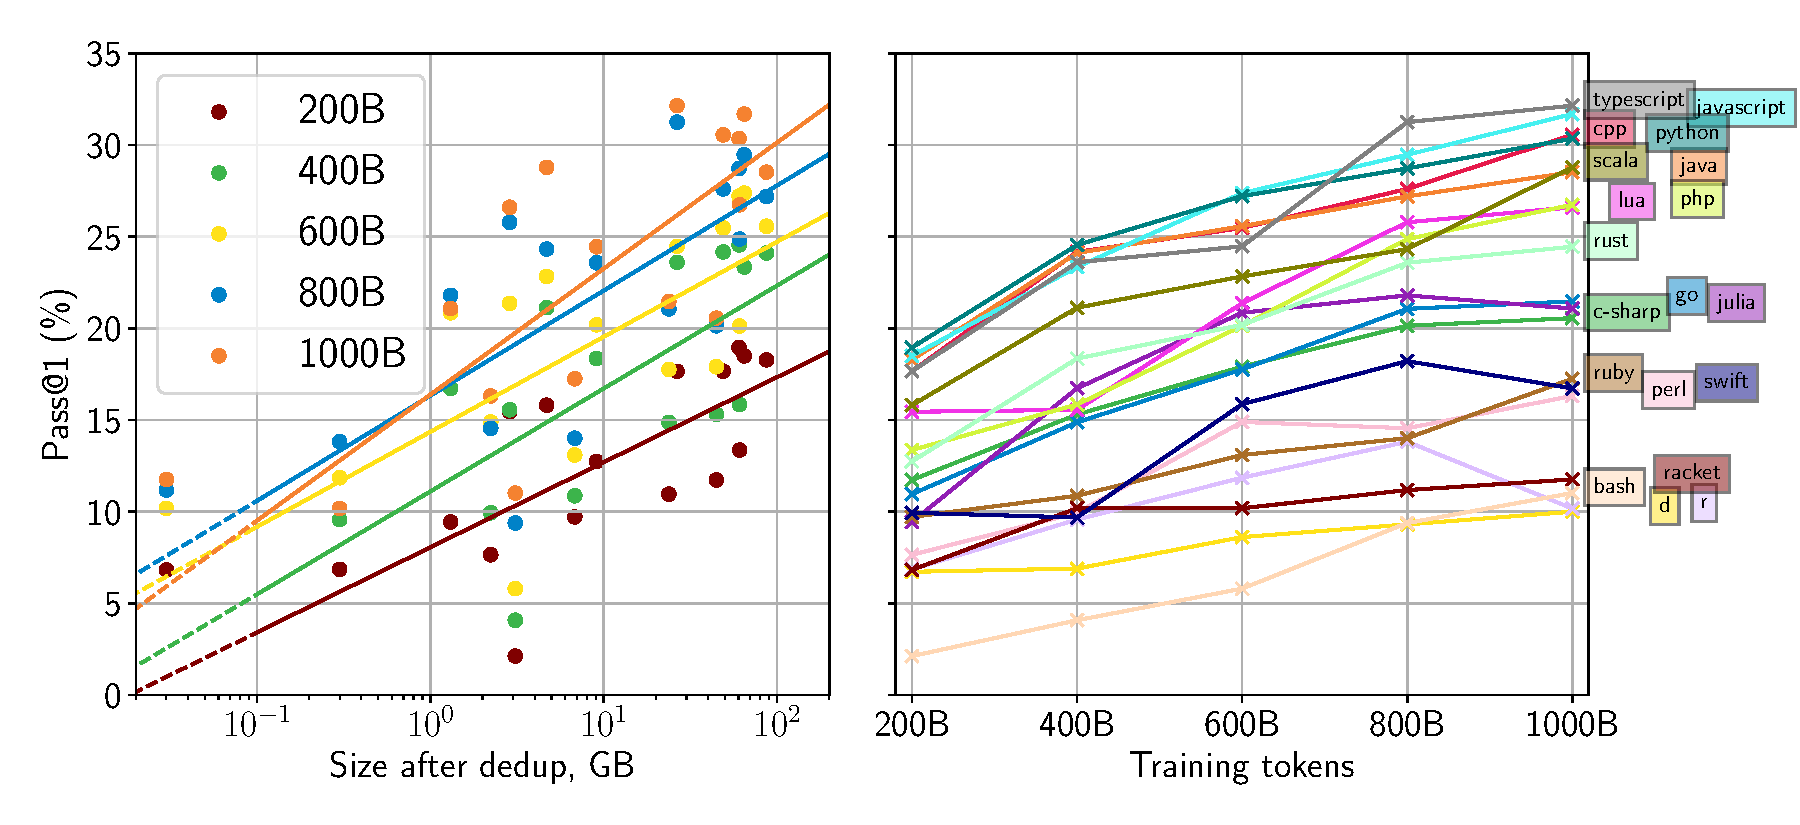
\includegraphics[width=\linewidth]{figures/performance.pdf}
	\caption{Performance (pass@1) of StarCoderBase at several training checkpoints  by data size \textbf{(left)} and by programming language \textbf{(right)}. The lines in the left plot are a linear fit between pass@1 and log-dataset-size for all the points except the leftmost one, where we expect the linear dependence to break due to transfer learning (dashed line). The goodness of fit ranges between $R^2=0.399$ for the 600B checkpoint to $R^2=0.510$ for the 1000B checkpoint. }
        \label{checkpoint-perf}
\end{figure*}

We evaluate the performance of StarCoderBase at several training checkpoints after every 200B tokens seen out of the total 1000B. Figure~\ref{checkpoint-perf} (right) shows how performance (pass@1) changes during training for each programming language supported by MultiPL-E. The performance curve for several high-resource programming languages suggests that training longer is likely to improve their performance further. 

However, some of the low-resource languages see limited improvement during training or even have a pass@1 decline. For example, R's pass@1 rate drops significantly between the 800B and 1000B (final) checkpoints. The dependence of pass@1 on data size (Figure~\ref{checkpoint-perf}, left) further supports the hypothesis that this is related to the amount of data available. The slope of the linear fit increases between 800B and 1000B checkpoints while the intercept decreases, i.e.,  performance improves only for languages with large enough amounts of data ($\gtrsim 1$ GB).

We manually inspected the completions generated by R over several checkpoints to better understand model performance. One might hypothesize that some problems are harder than others, and so the model gains and loses the ability to solve them in R over the 600B, 800B, and 1000B checkpoints, but we find that this is \emph{not} the case. Instead, we find significant variance in per-problem success rates for several problems (Table~\ref{apptab:Rcompletions}).
For these problems, the pass rate between different checkpoints varies in what appears to be a completely uncorrelated manner. Moreover, manual inspection shows that the failures are caused by minor mistakes,  e.g., not taking the absolute value when computing GCD, not converting a string to a character array, or not checking edge cases. 

\subsection{Perplexity With Long Contexts}

StarCoderBase was trained with an 8K token window, allowing conditioning on and generating long code files. To evaluate the ability of the model to benefit from this larger context, we compare its perplexity~\citep{bahl1983perplexity} when using a full window size of 8K tokens versus a window size of 2K tokens (as used in many prior code models).


To ensure no overlap between the training data for StarCoderBase and the perplexity computation data, we downloaded 10 GNU Public License (GPL) repositories
from GitHub in each of the languages in \autoref{tab:starcode_perplexity_benchmark}. We compiled all files from the repositories into a single document for each language. We then divided these documents into 8K token chunks and computed perplexity on the last 1K tokens in each chunk\footnote{We evaluate perplexity on the final 1K tokens in each 8K chunk so that both conditions have the same evaluation tokens, and to avoid overly penalizing the 2K condition, as tokens at the beginning of a window tend to have higher perplexity as there is less context available to predict them.} in two conditions: (1) the model window only contains the final 2K tokens in the chunk (i.e., the 1K being predicted and the previous 1K), and (2) the model window contains all 8K tokens in the chunk (i.e., the 1K tokens being predicted and the previous 7K). This evaluates the ability of the model to benefit from additional file- and repo-level context when predicting code.
In \autoref{tab:starcode_perplexity_benchmark}, we report the average perplexity of the 1K token regions across all chunks. We see that StarCoderBase indeed benefits from the extra token conditioning afforded by its 8K context window, with substantially lower perplexities across all languages.

\begin{table}[t]
\centering
\begin{tabular}{lcccccccccc}
\toprule
\multirow{2}{*}{\textbf{Window Size} } & \multicolumn{10}{c}{\textbf{Language}} \\ \cmidrule{2-11}
 & cpp & c-sharp & c & go & java & javascript & php & r & ruby & rust \\
\midrule

2K tokens & 2.01 & 1.90 & 1.71 & 1.35 & 1.65 & 1.98 & 1.73 & 1.72 & 2.16 & 1.84 \\
8K tokens & \textbf{1.79} & \textbf{1.66} & \textbf{1.61} & \textbf{1.21} & \textbf{1.54} & \textbf{1.68} & \textbf{1.43} & \textbf{1.48} & \textbf{2.02} & \textbf{1.65} \\
\bottomrule
\end{tabular}
\caption{Perplexity of StarCoderBase on evaluation regions (of size 1K tokens) when using a window size of 2K or 8K tokens across repositories from 10 languages. The larger window size substantially reduces perplexity, demonstrating a benefit of StarCoder's 8K token window.}
\label{tab:starcode_perplexity_benchmark}
\end{table}

\section{Natural Language Evaluation}

Although the StarCoder models are principally developed to be Code LLMs, they have also been trained on a significant amount of natural language text. Roughly 20\% of its training tokens are natural language data: 7\% GitHub issues, 10\% Markdown, 2\%  Jupyter notebooks, and 4\% HTML. 
% In this section, we evaluate StarCoderBase on several natural language understanding tasks.
In this section, we evaluate StarCoderBase on several natural language tasks: natural language reasoning and understanding tasks that might benefit from the combination of code and text training data; and natural language generation tasks that evaluate the model's tendencies to produce undesirable text outputs, e.g., in a documentation generation or interactive assistant setting.

\subsection{Math Reasoning}
% GSM8k only? 
Recent work has shown that Code LLMs can be effective arithmetic and symbolic reasoners by using a technique called Program-Aided Language models~\citep[PAL;][]{gao2022pal}. With PAL, the LLM reads the reasoning problem and generates Python programs as the intermediate reasoning steps, which are then executed by the Python  interpreter to produce the answer. In contrast, the Chain-of-Thought method~\citep[CoT;][]{wei2022chain} prompts the LLM to produce the reasoning steps in natural language before generating the answer.  

We investigate the reasoning capabilities of StarCoderBase on GSM8K~\citep{cobbe2021training}, a set of middle-school math word problems. We compare with the two CodeGen-16B models~\citep{nijkamp:codegen} and the family of LLaMA models~\citep{touvron2023llama}. The results of our evaluation are presented in Table~\ref{tab:gsm8k}, where we provide both CoT and PAL results for StarCoderBase and LLaMA.

In line with previous results comparing PAL to CoT on Code LLMs~\citep{gao2022pal}, we find that StarCoderBase performs better with PAL (21.5\%) than with CoT (8.4\%). StarCoderBase substantially outperforms CodeGen-16B-Mono and CodeGen-16B-Multi, which achieve 13.1\% and 8.6\% with PAL, respectively. These differences carry over to the setting where majority voting is applied.  The difference between CoT and PAL is much smaller for the LLaMA models, although we observe that CoT performs slightly better for the 7B and 13B LLaMA models. Interestingly, we find that StarCoderBase outperforms LLaMA-13B (17.8\%) on this reasoning benchmark. However, its performance still lags behind LLaMA-33B (38.7\%).   


\begin{table}
    \centering
    \begin{tabular}{rrcccc}
    \toprule 
    \textbf{Model} & \textbf{Size} & \textbf{GSM8K CoT} & \textbf{\small{\texttt{+maj1@100}}} & \textbf{GSM8K PAL} & \textbf{\small{\texttt{+maj1@40}}} \\
\midrule
%\cmidrule(r){1-2} \cmidrule(lr){3-4} \cmidrule(l){5-6}
    % BigCode - 40\% & 15B & & & & & 13.9 & \\
    % BigCode - 80\% & 15B & & & 10.1 & & 19.3 & 30.6 \\
    StarCoderBase & 15.5B & 8.4 & --- & 21.5 & 31.2 \\
\midrule
%\cmidrule(r){1-2} \cmidrule(lr){3-4} \cmidrule(l){5-6}
    CodeGen-Multi & 16B & 3.18 & --- & 8.6 & 15.2 \\
     CodeGen-Mono & 16B & 2.6 & --- & 13.1 & 22.4 \\
    % \midrule & 8B & 4.1 & - & - & -\\
    % PaLM & 62B & 33.0 & - & - & -\\
    % & 540B & 56.5 & - & - & - \\
    % \hline
    % & 8B & 16.2 & 28.4 & - & - \\
    % Minerva & 62B & 52.4 & 68.5 & - & - \\
    % & 540B & \textbf{58.8} & \textbf{78.5} & - & - \\
\midrule
%\cmidrule(r){1-2} \cmidrule(lr){3-4} \cmidrule(l){5-6}
   & 7B & 11.0 & 18.1 & 10.5 & 16.8 \\
    & 13B & 17.8 & 29.3 & 16.9 & 28.5 \\
    LLaMA & 33B & 35.6 & 53.1 & 38.7 & 50.3 \\
    & 65B & \textbf{50.9} & \textbf{69.7} & --- & ---\\
    % \midrule
    % code-davinci-002 & & \textbf{65.6} & \textbf{78.0} & \textbf{72.0} & \textbf{80.4} \\
    \bottomrule
    \end{tabular}
    \caption{8-shot accuracy on the GSM8K math-reasoning benchmark.
    Samples are generated with greedy decoding.
    \texttt{maj1@k} denotes a majority vote over $k$~generations.
    For the majority vote, we instead generate samples using nucleus sampling with $p=0.95$ and temperature $0.7$, following \citet{gao2022pal}. We use ``---'' when a model was not evaluated on a given metric, or the metric is not supported in \href{https://github.com/EleutherAI/lm-evaluation-harness}{Language Model Evaluation Harness}. The LLaMA CoT numbers are from~\citet{touvron2023llama}.} % The PaLM numbers are from~\citet{lewkowycz2022solving}, the code-davinci numbers are from~\citet{gao2022pal}}
    \label{tab:gsm8k}
\end{table}

\subsection{World Knowledge and Reading Comprehension}

MMLU~\citep{hendrycks2020mmlu} is a massive multitask language understanding benchmark, covering multiple-choice questions in 57 knowledge domains, including the humanities, STEM, and social sciences. CoQA~\citep{reddy2019coqa} is a large-scale dataset for Conversational Question Answering systems, measuring the model's ability to process a text passage and answer a series of interconnected questions. We compare StarCoderBase and StarCoder with CodeGen-16B-Multi~\citep{nijkamp:codegen}, GPT-NeoX~\citep{black2022gpt}, LLaMA-7B, and LLaMA-13B~\citep{touvron2023llama}. 

We present the 5-shot accuracy for MMLU in Table \ref{tab:mmlu}, and the zero-shot F1 scores for CoQA in Table \ref{tab:coqa}. On MMLU, StarCoderBase outperforms CodeGen-16B-Multi significantly (34.2\% to 27.8\%), and even outperforms GPT-NeoX by a small margin (32.9\%). Nevertheless, both LLaMA models outperform StarCoderBase.
On CoQA, StarCoderBase performs better than CodeGen-16B-Multi  but is outperformed by LLaMA and GPT-NeoX.


\begin{table}[t]
    \centering
    \begin{tabular}{rrc}
    \toprule
    \textbf{Model} & \textbf{Size} & \thead{\textbf{MMLU 5-shot}\\\textbf{acc, \%}} \\ 
    \midrule
    % \cmidrule(r){1-2} \cmidrule(l){3-3}
    CodeGen-Multi & 16B & 27.8 \\
    GPT-NeoX & 20B & 32.9 \\
    StarCoder & 15.5B & 33.9  \\
    StarCoderBase & 15.5B & 34.2  \\
    LLaMA & 7B & 35.1  \\
    LLaMA & 13B & \textbf{46.9} \\
    \bottomrule
    \end{tabular}
    \caption{5-shot accuracy on the MMLU language understanding benchmark.
     }
    \label{tab:mmlu}
\end{table}

\begin{table}[t]
    \centering
    \begin{tabular}{rrc}
    \toprule
    \textbf{Model} & \textbf{Size}  & \thead{\textbf{CoQA zero-shot}\\\textbf{F1 score}} \\
    \midrule
    % \cmidrule(r){1-2} \cmidrule(l){3-3}
    CodeGen-Multi & 16B & 0.59 \\
    StarCoderBase & 15.5B & 0.67  \\
    StarCoder & 15.5B & 0.67  \\
    LLaMA & 7B & 0.71  \\
    LLaMA & 13B & \textbf{0.73} \\
    GPT-NeoX & 20B & \textbf{0.73} \\
    \bottomrule
    \end{tabular}
    \caption{Zero-shot accuracy on the CoQA question answering challenge.
     }
    \label{tab:coqa}
\end{table}


% TODO: dfried
\subsection{Measuring Harmful Generation}
\label{sec:harmful_generations}
When generating open-ended text such as code documentation or technical dialogue, a Code LLM (similarly to text-only LLMs) might produce harmful outputs. We compare StarCoderBase to previous Code LLMs on benchmarks that measure social bias and toxicity
% , and hallucinations 
in model-produced text.\footnote{Code for the evaluations is available here: \url{https://github.com/McGill-NLP/StarCoderSafetyEval}}

\subsubsection{Social Bias}\label{sec:social_bias}

Recent work has highlighted that LLMs often capture social biases and stereotypes from their pre-training corpora \citep{kurita_measuring_2019,may_measuring_2019,hutchinson_social_2020,meade_using_2023}.
To quantify social bias within our model, we use StereoSet \citep{nadeem_stereoset_2021}.

StereoSet consists of a collection of fill-in-the-blank-style tests for measuring social biases within language models.\footnote{We only evaluate against the intrasentence task in this work.}
Each example in StereoSet consists of an incomplete sentence (e.g., \emph{our housekeeper is \texttt{BLANK}}) alongside three possible completions.
Of these completions, one is stereotypical (e.g., \emph{Mexican}), another is anti-stereotypical (e.g., \emph{Italian}) and a third is unrelated (e.g., \emph{computer}).
StereoSet defines three metrics: a stereotype score, a language modeling score, and an ICAT score.
The stereotype score is the percentage of examples for which a model \emph{prefers} the stereotypical completion for a sentence over the anti-stereotypical completion.
The language modeling score is the percentage of examples for which a model prefers a meaningful completion (stereotype or anti-stereotype) over an unrelated completion.
Finally, \citet{nadeem_stereoset_2021} define an idealized context association test (ICAT) score that combines these two metrics:
\begin{align}
 \mathrm{ICAT} = \mathrm{lms} \cdot \frac{\min(\mathrm{ss}, 100 - \mathrm{ss})}{50}
\end{align}
where $\mathrm{lms}$ and $\mathrm{ss}$  denote the language model score and stereotype score, respectively.

We report StereoSet results for StarCoderBase, alongside LLaMA-13B and CodeGen-Multi-16B, in Table~\ref{tab:stereoset}.
Across all four bias domains, we find StarCoderBase obtains the lowest stereotype scores, but also has competitive language modeling scores. 
%For instance, StarCoderBase obtains a stereotype score of $58.76\%$ in the gender domain while CodeGen-16B-Multi obtains a stereotype score of $67.34\%$.
%Importantly, StarCoderBase also obtains competitive language modeling scores.
This suggests that StarCoderBase's lower stereotype scores are not simply due to worse language modeling \citep{meade_empirical_2022}, and also as indicated by the high ICAT score.

We also evaluate StarCoderBase against Crowdsourced Stereotype Pairs (CrowS-Pairs; \citealt{nangia_crows-pairs_2020}) and refer readers to Table~\ref{tab:crows_pairs} for results.

\begin{table}[t]
    \centering
    \begin{tabular}{lccc}
        \toprule
        \textbf{Model} & \textbf{Stereotype Score} & \textbf{Language Model Score} & \textbf{ICAT Score} \\
        \midrule
        %\cmidrule(r){1-1} \cmidrule(l){2-4}
        % & \multicolumn{3}{c}{\emph{Gender}} \\
        & & \emph{Gender} \\
        \midrule
        %\cmidrule(r){1-1} \cmidrule(l){2-4}
        LLaMA-13B & 66.54 & \textbf{88.09} & 58.95 \\
        CodeGen-Multi-16B & 67.34 & 86.41 & 56.44 \\
        StarCoderBase & \textbf{58.76} & 86.82 & \textbf{71.60} \\
        \midrule
        %\cmidrule(r){1-1} \cmidrule(l){2-4}
        % & \multicolumn{3}{c}{\emph{Profession}} \\
        & & \emph{Profession} \\
        \midrule
        %\cmidrule(r){1-1} \cmidrule(l){2-4}
        LLaMA-13B & 60.95 & \textbf{86.74} & 67.74 \\
        CodeGen-Multi-16B & 60.67 & 85.67 & 67.38 \\
        StarCoderBase & \textbf{53.24} & 84.70 & \textbf{79.21} \\
        % \midrule
        \midrule
        %\cmidrule(r){1-1} \cmidrule(l){2-4}
        % & \multicolumn{3}{c}{\emph{Race}} \\
        & & \emph{Race} \\
        % \midrule
        \midrule
        %\cmidrule(r){1-1} \cmidrule(l){2-4}
        LLaMA-13B & 64.94 & 87.97 & 61.68 \\
        CodeGen-Multi-16B & 60.58 & \textbf{88.60} & 69.85 \\
        StarCoderBase & \textbf{56.48} & 86.82 & \textbf{75.58} \\
        % \midrule
        \midrule
        %\cmidrule(r){1-1} \cmidrule(l){2-4}
        % & \multicolumn{3}{c}{\emph{Religion}} \\
        & & \emph{Religion} \\
        \midrule
        %\cmidrule(r){1-1} \cmidrule(l){2-4}
        % \midrule
        LLaMA-13B & 57.95 & 90.26 & 75.91 \\
        CodeGen-Multi-16B & 56.16 & 88.91 & 77.96 \\
        StarCoderBase & \textbf{55.69} & \textbf{90.67} & \textbf{80.36} \\
        % \midrule
        \midrule
        %\cmidrule(r){1-1} \cmidrule(l){2-4}
        % & \multicolumn{3}{c}{\emph{Overall}} \\
        & & \emph{Overall} \\
        % \midrule
        \midrule
        %\cmidrule(r){1-1} \cmidrule(l){2-4}
        LLaMA-13B & 63.40 & \textbf{87.62} & 64.14 \\
        CodeGen-Multi-16B & 61.29 & 87.25 & 67.55 \\
        StarCoderBase & \textbf{55.53} & 86.18 & \textbf{76.65} \\
        \bottomrule
    \end{tabular}
    \caption{StereoSet intrasentence results for gender, professional, racial, and religious bias. Stereotype scores close to 50\% are best. Language modeling scores and ICAT scores close to $100\%$ are best.}
    \label{tab:stereoset}
\end{table}

\subsubsection{Toxicity}\label{sec:toxicty}
To evaluate toxicity in responses generated from our model, we use RealToxicityPrompts \citep{gehman_realtoxicityprompts_2020}, a collection of sentence-level prompts that often elicit undesirable responses from language models.
We generate responses to 10K examples from RealToxicityPrompts using StarCoderBase with a minimum length of one token and a maximum length of $128$ tokens.
We use nucleus sampling~\citep{holtzman2020curious} with $p = 0.95$ to generate all of our responses.

We use two methods for automatically evaluating toxicity in responses: (i) a RoBERTa-based \citep{liu2019roberta} toxicity classifier \citep{vidgen_learning_2021} and (ii) a list of potentially offensive words.\footnote{\url{https://github.com/LDNOOBW/List-of-Dirty-Naughty-Obscene-and-Otherwise-Bad-Words}}
For the toxicity detector, we report the percentage of responses flagged toxic using a threshold of $0.5$. 
For the offensive word list, we report the percentage of responses which contain an offensive word.
We note that while the offensive word list can potentially falsely flag responses, it may provide a crude measure of blatant toxicity.
We report our results in Table~\ref{tab:real_toxicity_prompts}. 

In general, we observe that CodeGen-16B-Multi and StarCoderBase both appear to generate less toxic responses than LLaMA-13B.
For instance, $1.43\%$ of LLaMA-13B's responses contain potentially offensive tokens compared to the $1.12\%$ of StarCoderBase.
We also note that CodeGen-16B-Multi appears to generate less toxic responses than StarCoderBase.

\begin{table}[t]
    \centering
    \begin{tabular}{lcc}
        \toprule
        \textbf{Model} & \textbf{Classifier} & \textbf{Word List} \\
        \midrule
        % \cmidrule(r){1-1} \cmidrule(l){2-3}
        LLaMA-13B & 0.74 & 1.43 \\
        CodeGen-Multi-16B & \textbf{0.21} & \textbf{0.82} \\
        StarCoderBase & 0.42 & 1.12 \\
        \bottomrule
    \end{tabular}
    \caption{RealToxicityPrompts response toxicity results. We report the percentage of responses flagged as toxic using a toxicity classifier and an offensive word list. Lower scores are indicative of less toxic generations.}
    \label{tab:real_toxicity_prompts}
\end{table}

% \subsubsection{Hallucinations}\label{sec:hallucinations}

% LLMs are prone to generating factually incorrect or unverifiable statements \citep{rashkin_increasing_2021,dziri-etal-2022-origin,ji_survey_2023,liu_evaluating_2023}.
% To evaluate hallucinations in responses from our model, we use FaithDial~\citep{dziri_faithdial_2022}: a collection of dialogues from the Wizard of Wikipedia dataset~\citep{dinan_wizard_2019} which have been edited to remove hallucinations.
% We generate responses to FaithDial in an \emph{oracle} setting where we provide the required knowledge for response generation in-context using the prompt below:
% \begin{verbatim}
% Answer the following question using the following knowledge:

% Knowledge: <knowledge>

% Conversation:
% User: <question>
% Assistant:
% \end{verbatim}
% We note that the conversation can potentially consist of multiple conversation turns between \verb|User| and \verb|Assistant|. 
% We generate responses with a minimum length of one token and a maximum length of $128$ tokens and use Nucleus Sampling with $p = 0.95$ for sampling all responses.
% Following response generation, we use a RoBERTa-based hallucination critic to quantify whether the generated responses are grounded in the provided knowledge.
% We report the percentage of responses flagged as hallucinations by the critic.

% In Table~\ref{tab:faithdial}, we report results for LLaMA-13B, CodeGen-16B-Multi and StarCoderBase.
% We find that all three code models generate a large amount of hallucinated responses ($>75\%$) with LLaMA-13B performing best ($76.24\%$).
% We hypothesize that this poor performance is due to the models not being instruction-tuned.
% In most cases, we found the responses did not reference the provided knowledge in any form.

% \begin{table}[t]
%     \centering
%     \begin{tabular}{lr}
%         \toprule
%         \textbf{Model} & \textbf{Hallucination Critic}  \\
%         \midrule
%         LLaMA-13B & 76.26 \\
%         CodeGen-Multi-16B & 80.22 \\
%         StarCoder & 81.80 \\
%         \bottomrule
%     \end{tabular}
%     \caption{FaithDial hallucination critic results. We report the percentage of responses flagged as hallucinations using a trained critic. Lower scores are indicative of less hallucinations across the responses.} 
%     \label{tab:faithdial}
% \end{table}

\subsection{Reasoning Tasks in HELM}
% \subsubsection{Reasoning Tasks in HELM}
% %Please add the following packages if necessary:
%\usepackage{booktabs, multirow} % for borders and merged ranges
%\usepackage{soul}% for underlines
%\usepackage[table]{xcolor} % for cell colors
%\usepackage{changepage,threeparttable} % for wide tables
%If the table is too wide, replace \begin{table}[!htp]...\end{table} with
%\begin{adjustwidth}{-2.5 cm}{-2.5 cm}\centering\begin{threeparttable}[!htb]...\end{threeparttable}\end{adjustwidth}

% without average rank column
\begin{table}
\centering
% \caption{Generated by Spread-LaTeX}\label{tab: }
% https://docs.google.com/spreadsheets/d/1Kra9d2UdfvdW3AoO3oqdAlOgQocWXqpqf3jtn20BvoU/edit?usp=sharing
\scriptsize
% \begin{tabularx}{1.06\linewidth}{Xccccccccccc}
\begin{tabular}{p{0.15\textwidth}ccccccccccc}
\toprule
% &\multirow{3}{*}{\textbf{Synthetic\\Reasoning:\\Abstract}} &\multirow{3}{*}{\textbf{Synthetic\\Reasoning:\\NL}} &\textbf{bAbI} &\textbf{Dyck} &\textbf{GSM8K} &\textbf{MATH} & \multirow{3}{*}{\textbf{MATH (chain-of-thought)}} &\textbf{LSAT - EM} &\textbf{LegalSupport} &Average Rank \\
% &\thead{\textbf{Synthetic\\Reasoning:\\Abstract}} &\thead{\textbf{Synthetic\\Reasoning:\\NL}} &\textbf{bAbI} &\textbf{Dyck} &\textbf{GSM8K} &\textbf{MATH} & \thead{\textbf{MATH\\(CoT)}} &\thead{\textbf{LSAT\\EM}} &\thead{\textbf{Legal\\Support}} & \thead{Average\\Rank} \\
\textbf{Model} & \thead{\textbf{Weights}\\\textbf{Released}} &\thead{\textbf{Synth.}\\\textbf{Reason.}\\\textbf{AS}} &\thead{\textbf{Synth.}\\\textbf{Reason:}\\\textbf{NL}} &\thead{\textbf{bAbI}} &\thead{\textbf{Dyck}} &\thead{\textbf{GSM8K}} &\thead{\textbf{MATH}} & \thead{\textbf{MATH}\\\textbf{(CoT)}} &\thead{\textbf{LSAT}} &\thead{\textbf{Legal}\\\textbf{Support}} \\
%\cmidrule(r){1-1} \cmidrule(l){2-11}
\midrule
code-davinci-002 & &\textbf{0.54} &0.684 &\textbf{0.686} &0.805 &\textbf{0.568} &\textbf{0.41} &0.433 &--- &--- \\
text-davinci-003 & &0.502 &\textbf{0.734} &0.653 &0.751 &0.506 &0.39 &\textbf{0.449} &\textbf{0.233} &\textbf{0.622} \\
Luminous Supreme (70B) & &0.312 &--- &0.504 &0.729 &0.112 &0.149 &0.057 &0.212 &0.53 \\
StarCoderBase (15.5B) & \checkmark &0.44 &0.21 &0.504 &\textbf{0.854} &0.084 &0.151 &0.07 &0.19 &0.532 \\
Cohere Command Beta (52.4B) & &0.243 &0.245 &0.473 &0.421 &0.138 &0.133 &0.075 &0.229 &0.606 \\
J1-Jumbo v1 (178B) & &0.263 &0.174 &0.543 &0.445 &0.054 &0.089 &0.033 &0.232 &0.484 \\
J1-Grande v2 beta (17B) & &0.286 &0.139 &0.47 &0.617 &0.096 &0.127 &0.068 &0.191 &0.562 \\
code-cushman-001 & &0.341 &0.164 &0.481 &0.451 &0.049 &0.099 &0.072 &--- &--- \\
OPT (175B) & \checkmark &0.225 &0.248 &0.507 &0.494 &0.04 &0.065 &0.026 &0.22 &0.532 \\
GPT-NeoX (20B) & \checkmark & 0.204 &0.167 &0.468 &0.747 &0.053 &0.141 &0.071 &0.191 &0.515 \\
BLOOM (176B) & \checkmark &0.304 &0.197 &0.447 &0.545 &0.095 &0.043 &0.055 &0.209 &0.543 \\
GLM (130B) & \checkmark &0.252 &0.254 &0.443 &0.549 &0.061 &0 &0.059 &0.193 &0.451 \\
UL2 (20B) & \checkmark &0.205 &0.217 &0.501 &0.14 &0.024 &0 &0 &0.207 &0.506 \\
OPT (66B) & \checkmark &0.193 &0.213 &0.408 &0.471 &0.018 &0.048 &0.029 &0.175 &0.527 \\
YaLM (100B) & \checkmark &0.056 &0.061 &0.346 &0.633 &0 &0 &0 &0.23 &0.484 \\
T5 (11B) & \checkmark &0.196 &0.101 &0.412 &0.347 &0.023 &0 &0 &0.159 &0.558 \\
\bottomrule
% \end{tabularx}
\end{tabular}
\caption{Model results on natural language reasoning tasks in the HELM benchmark, with models ordered by their average rank on the tasks. We use ``---'' when a model was not evaluated on a given metric, or has runtime errors logged in HELM (e.g., ``unmapped prediction'' for the code-davinci-002 and code-cushman-001 models on LSAT and Legal Support). StarCoder generally substantially outperforms other models with released weights, and often outperforms much larger models.}
\label{tab:helm_results}
\end{table}
%Please add the following packages if necessary:
%If the table is too wide, replace \begin{table}[!htp]...\end{table} with
%\begin{adjustwidth}{-2.5 cm}{-2.5 cm}\centering\begin{threeparttable}[!htb]...\end{threeparttable}\end{adjustwidth}

% without average rank column
\begin{table}
\centering
% \caption{Generated by Spread-LaTeX}\label{tab: }
% https://docs.google.com/spreadsheets/d/1Kra9d2UdfvdW3AoO3oqdAlOgQocWXqpqf3jtn20BvoU/edit?usp=sharing
\scriptsize
\setlength{\tabcolsep}{3pt}
% \begin{tabularx}{1.06\linewidth}{Xccccccccccc}
\resizebox{\textwidth}{!}{
\begin{tabular}{p{0.14\textwidth}rcccccccccccc}
\toprule
\textbf{Model} & \multicolumn{1}{c}{\textbf{Size}} &
% \thead{\textbf{Weights}\\\textbf{Released}}
\thead{\textbf{Open}\\\textbf{Access}}
&\thead{\textbf{Synth.}\\\textbf{Reason.}\\\textbf{(AS)}} &\thead{\textbf{Synth.}\\\textbf{Reason.}\\\textbf{(NL)}} &\thead{\textbf{bAbI}} &\thead{\textbf{Dyck}} &\thead{\textbf{GSM8K}} & {\textbf{MATH}} & \thead{\textbf{MATH}\\\textbf{(CoT)}} &\thead{\textbf{LSAT}} &\thead{\textbf{Legal}\\\textbf{Support}} \\
\midrule
code-davinci-002 & 175B & &\textbf{54.0} &68.4 &\textbf{68.6} &80.5 &\textbf{56.8} &\textbf{41.0} &43.3 &--- &--- \\
text-davinci-003 & 175B & & 50.2 &\textbf{73.4} &65.3 &75.1 &50.6 &39.0 &\textbf{44.9} &\textbf{23.3} &\textbf{62.2} \\
Luminous Supreme & 70B & & 31.2 &--- &50.4 &72.9 &11.2 &14.9 &5.7 &21.2 &53.0 \\
StarCoderBase & 15.5B & \checkmark &44.0 &21.0 &50.4 &\textbf{85.4} & 8.4 &15.1 &7.0 &19.0 &53.2 \\
Cohere Command Beta & 52.4B & &24.3 &24.5 &47.3 &42.1 &13.8 &13.3 &7.5 &22.9 &60.6 \\
J1-Jumbo v1 & 178B & &26.3 &17.4 &54.3 &44.5 &5.4 &8.9 &3.3 &23.2 &48.4 \\
J1-Grande v2 beta & 17B & &28.6 &13.9 &47.0 &61.7 &9.6 &12.7 &6.8 &19.1 &56.2 \\
code-cushman-001 & 12B & &34.1 &16.4 &48.1 &45.1 &4.9 &9.9 &7.2 &--- &--- \\
OPT & 175B & \checkmark &22.5 &24.8 &50.7 &49.4 &4.0 &6.5 &2.6 &22.0 &53.2 \\
GPT-NeoX & 20B & \checkmark & 20.4 &16.7 &46.8 &74.7 &5.3 &14.1 &7.1 &19.1 &51.5 \\
BLOOM & 176B & \checkmark &30.4 &19.7 &44.7 &54.5 &9.5 &4.3 & 5.5 &20.9 &54.3 \\
GLM  & 130B & \checkmark &25.2 &25.4 &44.3 &54.9 &6.1 &0 &5.9 &19.3 &45.1 \\
UL2  & 20B & \checkmark &20.5 &21.7 &50.1 &14.0 &2.4 &0 &0 &20.7 &50.6 \\
OPT  & 66B & \checkmark &19.3 &21.3 &40.8 &47.1 &1.8 &4.8 &2.9 &17.5 &52.7 \\
YaLM & 100B & \checkmark &5.6 &6.1 &34.6 &63.3 &0 &0 &0 &2.3 &48.4 \\
T5  & 11B & \checkmark &19.6 &10.1 &41.2 &34.7 &2.3 &0 &0 &15.9 &55.8 \\
\bottomrule
\end{tabular}
}
% qian: change weights released to open access to keep consistency with previous mention
\caption{Model results on natural language reasoning tasks in the HELM benchmark, with models ordered by their average rank on the tasks. We use ``---'' when a model was not evaluated on a given metric, or has runtime errors logged in HELM (e.g., ``unmapped prediction'' for the code-davinci-002 and code-cushman-001 models on LSAT and Legal Support). StarCoder generally substantially outperforms other open-access models, and often outperforms much larger models.}
\label{tab:helm_results}
\end{table}

We evaluate StarCoderBase with HELM~\citep{liang2022helm}, an evaluation suite aiming to increase the transparency of LLMs by reporting their performance on a wide range of tasks. 
We evaluate the ability of the model to leverage its natural language and code pretraining for natural language \emph{reasoning} tasks from HELM (excluding code tasks, because of our own extensive code evaluations).
At the time of writing, the HELM benchmark does not include the CodeGen, CodeGeex, and LLaMA models. Therefore, we compare StarCoderBase with the largest and/or most recent model from each family of ``limited'' or ``open'' access models, as classified on the HELM model list,\footnote{\url{https://crfm.stanford.edu/helm/latest/?models=1}} that had been evaluated on a majority of these HELM reasoning tasks as of May 1, 2023.  In Table~\ref{tab:helm_results} we report the results. We compute each model's ranking on each task, and order models in the table by their average ranking across tasks. StarCoderBase generally obtains substantially stronger performance than all other models with released weights and often performs comparably to or better than much larger models. We speculate that the mixture of code and natural language in the training data contributes to the model's strong performance on these reasoning tasks.


\section{Qualitative Evaluation}
\lstset{basicstyle=\footnotesize\ttfamily}
In \autoref{app:qualitative}, we highlight several interesting interactions we had with StarCoderBase. We hope these serve as a  starting point for researchers and developers interested in further exploring the model's capabilities.
We provide examples of how to elicit interesting model behavior using the templates for Git commits, GitHub issues, and Jupyter notebooks in Section \ref{sec:pretraining_templates}. In Section \ref{sec:technical_assistant}, we demonstrate how to prompt StarCoder to act as a technical assistant without any instruction-tuning. In Section~\ref{sec:prompting} we find that it is also possible to prompt the model using a combination of meta-data and natural language to obtain higher pass@1 performance on the HumanEval benchmark.

% from the intro:
% We incorporate a new attribution tool into the VSCode demo that can help users detect
% and locate model generations which may have been copied from the training set. This
% is achieved through a two-step process that involves a lightweight membership check
% followed by a search over a BM25 index. See Section 8.

\section{Attribution Tools}\label{sec:attribution_tool}
As generative language tools become more ubiquitous and data-intensive, the need to understand and inspect the massive amounts of text they were trained on becomes more pressing, both to understand the failure modes of models as well as provide transparent data governance feedback in the form of attribution tracing and provenance management of a model's generated output. This pressing need for understanding data~\citep{mitchell-measuring-data} is being increasingly recognized and operationalized in the form of dataset inspection tools and toolkits~\citep{akiki-spacerini-search,marone-data-portraits-search,piktus-roots-search}.
It is from this vantage point that we are releasing two such data inspection tools: a membership-checking tool and a BM25 search index.
These complement the existing ``Am I in The Stack'' tool which operates at the level of GitHub repository names. % \footnote{\url{https://huggingface.co/spaces/bigcode/in-the-stack}}
The two new tools index only the files used for training and allow for matches on file content.
These tools are available as standalone sites but are also integrated into our VSCode demo.
This helps users identify parts of the model output that may have been copied from the training data. By utilizing the search index, users can locate the corresponding source file and repository of the copied snippets. 

\subsection{Membership Checking}
\citet{marone-data-portraits-search} propose documenting datasets with membership testing artifacts deemed \emph{Data Portraits}.
They provide one specific implementation, based on Bloom Filters \citep{bloom-filters-10.1145/362686.362692}, that offers fast and lightweight membership inference.
We build a Bloom-filter-based portrait on strings of length 50 characters from the training data.
This artifact takes 26 GB, $\sim3\%$ of the data size.
The inference tool is hosted publicly to complement other documentation artifacts. \footnote{\url{http://stack.dataportraits.org/}}

Generations from the model can be quickly checked to approximately assess the degree of overlap with the training corpus.
The VSCode extension supports using this as a rapid, first-pass attribution method.
However, this requires that matching strings are longer than a minimum size and does not attempt to filter common or generic code snippets.
After the first pass check, users can use the full search index to further assess attribution. 

\subsection{Search Index}
We index the training dataset using Elasticsearch~7.17\footnote{\url{https://www.elastic.co/guide/en/elasticsearch/reference/7.17}} and provide two search tools to query it: one focused on the Python subset and one covering the entire dataset.
%\footnote{\url{https://hf.co/spaces/bigcode/py-search}}\footnote{\url{https://hf.co/spaces/bigcode/search}} 
The code itself is preprocessed using a lowercase filter and Lucene's \texttt{ASCIIFoldingFilter}, tokenized using a 3-gram tokenizer, and indexed using the default Lucene implementation of BM25 as a similarity function. We further index the username and license fields as \texttt{keyword} fields allowing for easy filtering and lookup based on these specific metadata fields. Both indexes are currently running in single-node mode on one virtual machine.

\section{Social Impact and Limitations}

\subsection{Project approach}

\paragraph{Open-science and open-governance} StarCoder is an output of a community research project. The project is conducted in the spirit of Open Science~\citep{open-science}, focused on the responsible development \emph{and} use of Code LLMs. Through open-governance practices conducted throughout the project, priority in decision-making has always yielded to the more responsible option even if this meant introducing limitations that might impact adoption or future research. For example, the Legal, Ethics, Governance Working Group decided to remove and not release a dataset of identified malicious code, even though this data might be useful for future security research.
% The Working Group felt that such code already exists in places already well known to security researchers, and did not need to remain in The Stack.

\paragraph{Openness and safety risks}
\citet{solaiman2023gradient} explains how the degree of openness in the LLM development process is connected to the potential risks associated with a model release. When systems are developed in a fully closed manner, it is more likely for power to become concentrated among high-resourced organizations, and the small development team may not fully comprehend the impact and long-term consequences of the model being deployed. In addition, closed-development systems are often less auditable by external experts and can impede scientific progress since researchers cannot build upon each other's work. On the other hand, fully open development allows for community research, democratizes access to the models, and enables audits throughout the whole development process. However, without appropriate guardrails, open LLM development poses a higher risk of misuse, as increased model access also increases the likelihood of harm caused by the model. Even though a released API can be shut down, once the model weights are released, it is nearly impossible to retract them.  Discussing and implementing responsible AI practices has, therefore, been front and center during the  development of our project's LLMs.

% By releasing StarCoder with an Open Responsible AI Model license along with the model weights, and by open-sourcing all code repositories on GitHub,\footnote{\url{https://github.com/bigcode-project}} (including the model training framework, the dataset filtering methods, the code evaluation suite, and the research analysis notebooks), we aim to increase access, reproducibility, and transparency of Code LLMs in the research community. It is important to note that Appendix A of the model license includes the use restrictions set by the BigCode community to ensure that modifications of the model, and applications using the model, adhere to the BigCode principles of responsible AI.

\subsection{Limitations}
\paragraph{Dataset and data licensing} StarCoder was trained on a subset of The Stack v1.2 dataset. % \footnote{\url{https://huggingface.co/datasets/bigcode/the-stack}} 
This dataset has been filtered using a license detector to only include permissively licensed source code. Nevertheless, the license detector might have incorrectly classified a number of repositories. See \citet{Kocetkov2022TheStack} for more details on this license detection process. 

% Nevertheless, the license detector might have incorrectly classified a number of repositories. Please reach out to \url{contact@bigcode-project.org} in case StarCoder generates verbatim copies of non-permissively licensed source code or if you encounter files in The Stack that do not have a permissive license. 

%See The Stack~\citep{Kocetkov2022TheStack} for details of the limitations, including the Social impact of the dataset, Biases of the dataset, HTML not WCAG compliant, PII, Malicious code, and Data licensing.


\paragraph{Opt-out process} Although The Stack offers a way to remove developer code, its opt-out process only applies to individual repositories and could benefit from further enhancements. For example, when code is licensed under a permissive or copy-left license, it can be duplicated to another repository, making it challenging to eliminate such copies if the copyright owner chooses to opt out. More work is necessary to create better data control and consent mechanisms for large-scale training sets of LLMs. 

 
\paragraph{PII detection} Despite our best efforts to remove PII (Section \ref{sec:PII}), StarCoder may still produce PII (however, note that the model license restricts use that aims to generate or disseminate PII with the purpose of harming others). As mentioned in Section~\ref{sec:bigcode_encoder}, %4 . 2 S TA R E N C O D E R,%
we trained an encoder-only model to detect PII for both code- and text-related tasks and noted that there is a possibility of false positives and negatives, which could lead to unintended consequences when processing sensitive data. Moreover, the PII detection model's performance may vary across different data types and programming languages, necessitating further validation and fine-tuning for specific use cases. The PII annotations are only available to approved individuals, and researchers and developers who are granted access are expected to uphold ethical standards and data protection measures. By making it accessible, our aim is to encourage further research and development of PII redaction technology. 

\paragraph{Malicious code} On the Hugging Face platform, where the Stack is hosted, a malicious code detection tool identified 654 files as unsafe. With the help of our community, we removed these files ahead of the release of The Stack v1.2. Nevertheless, The Stack may contain undetected malicious code, and StarCoder might be able to generate malware. The StarCoder OpenRAIL-M license, therefore, includes a use restriction against generating and/or disseminating malware (including --- but not limited to --- ransomware) or any other content that can be used to harm electronic systems.

\paragraph{Model limitations} StarCoder is subject to typical limitations of LLMs, including the potential to generate  content that is inaccurate, offensive, misleading, discriminatory towards age or gender, or reinforces other stereotypes. Please refer to Section \ref{sec:harmful_generations} for an investigation into such safety concerns. Deployments of StarCoder need to further challenge and adapt the model to prevent such behavior, e.g., through red-teaming~\citep{perez2022red}, adversarial testing \citep{wan2023poisoning}, and/or by adding a robust safety layer~\citep{openai2023systemcard}. The model is released with an OpenRAIL-M license that places enforceable use restrictions that apply to the model and its modifications, and to applications using the model. 

%Safety-critical applications may benefit from additional safeguards such as Dialog-Enabled Resolving Agents \citep{nair2023dera} to ensure that generated outputs are more factually accurate and complete. It may also be advantageous to train Code LLMs to self-debug \citep{chen2023teaching} or evaluate code quality~\citep{zhuo2023large}. 

\paragraph{English-only evaluations} We evaluated the performance of StarCoder solely on English-based benchmarks to understand its coding capabilities and natural language understanding. To make these models more accessible to a wider audience, future research should investigate the performance and limitations of Code LLMs on other natural languages. 

\paragraph{Code attribution tools} The StarCoder membership-checking tool and BM25 search index are limited to dataset inspection against the subset of The Stack that was used for training and, as such, will not find matches to code that was not included or that was removed from the dataset for this project. The Portraits-based membership testing tool uses hash matching and thus may have false positives. It also has a minimum resolution and requires a certain amount of context to trigger a match. 
Both attribution tools do not attempt to distinguish between generic code (e.g., boilerplate) or protected content. However, we hope that these tools will support ongoing research on the responsible development of LLMs.
% These tools support ongoing research that support the responsible development of LLMs.


\subsection{Social impact}

\paragraph{Code LLMs} We expect Code LLMs to enable people from diverse backgrounds to learn to write higher-quality code and develop
low-code applications \citep{leinonen2023comparing}. Mission-critical software could become easier to maintain as professional developers are guided by code-generating systems on how to write more robust and efficient code. However, the security implications should also be carefully considered \citep{sandoval2023lost}. While the social impact is intended to be positive, the increased accessibility of Code LLMs comes with certain risks such as over-reliance on the generated code and long-term effects on the software development job market. We refer the reader to \citet[Section 7]{chen2021codex} for a broader impact analysis of Code LLMs, as well as \citet{khlaaf2022hazard} for an in-depth risk assessment and hazard analysis of this emerging technology.

\paragraph{Data annotation} It was important for the project to only use reputable data annotation services. It was also important to balance the constraints of costs (fair compensation), time (the timing and time to complete the work were on the critical path for the project), and quality (to ensure that PII Detection Model training was not impacted). While traditional data annotation services using salaried employees were considered, the decision to work with Toloka crowd-workers was taken after a review of service providers and their compensation practices --- most would not provide sufficient transparency and guarantees about worker compensation. Our determination of compensation took into consideration different minimum wage rates across countries and their corresponding purchasing power. We limited annotation eligibility to countries where the hourly pay rate of \$7.30 was equivalent to the highest minimum wage in the US (\$16.50) in terms of purchasing power parity. 

\paragraph{Feedback opt-out form}
During the first stage of the opt-out process, individuals were asked to specify the reasons for wanting their code to be excluded from the dataset. The recurring concerns we heard from the individual who wished to opt out are:
\begin{itemize}
    \item Preference for an opt-in approach instead of opt-out.
    \item Perception that it is unfair to use their code without compensation
    \item Concerns about the current limitations of AI and the potential for model generations to be traced back to their work, resulting in potential legal liability.
    \item Belief that their code is of poor quality and unsuitable for AI training.
    \item Presence of PII in their code, which they do not wish to be publicly exposed.
\end{itemize}
The opt-out form thus provided an opportunity to directly engage with content creators and learn about the impact of our work on them.  
%The release of governance tools like ``Am I in The Stack'' tool\footnote{\url{https://huggingface.co/spaces/bigcode/in-the-stack}} provided an opportunity to directly engage communities in conversation about the process and impact of LLMs in a practical, rather than hypothetical, way.

\paragraph{Community feedback on opt-out process}
We conducted community research with individuals at specific organizations whose data is used in The Stack (\href{https://turing.ac.uk/}{The Alan Turing Institute} and \emph{\href{https://the-turing-way.netlify.app/}{The Turing Way}}) and contributed to two open, international workshops (\href{https://opendataday.org/events/2023/#designing-for-data-rights-in-the-ai-production-pipeline}{Open Data Day 2023} and \href{https://schedule.mozillafestival.org/session/KAS9YF-1}{Mozilla Festival 2023} with a session titled ‘Designing for Data Rights in the AI Production Pipeline’). 
These qualitative interviews and participatory co-design workshops included 50 participants, primarily from North America and Europe, with roles including research scientist, community manager, software engineer, and principal investigator (PI).

The outcomes from the community research can be summarized as follows: when it comes to governance of LLM datasets, participants feel that it is both \emph{better to know} and \emph{better to have a choice}. Most participants had neutral to positive feelings about their permissively licensed data being used to train LLMs. While all had positive impressions of the ``Am I in The Stack'' tool, not one interviewed expressed a desire to actually opt out. The main takeaway seemed to be that participants found the most value in the project's governance tools for their ability to raise awareness of data practices and to empower individuals and communities to take action based on their specific needs. These initial conversations also highlighted the importance of bringing governance discussions and decisions directly to impacted communities, an important direction of future work that should extend community research beyond North America and Europe. Participants in the workshops also raised examples of new groups to center in data rights considerations, including artists, data miners, and future generations. The co-created outputs can be viewed on this \href{https://github.com/bigcode-project/bigcode-analysis/blob/main/community_research/mozfest.pdf}{MozFest Miro Board}.




% Investigation into the natural language could be elaborated, now mainly focus on programming language aspect... Does not cover all code languages from The Stack
% Performance and experiments were timeboxed to fit the project, room for improvement
% Base model vs. RLHF
% Code LLM safety and trust tools
% Malicious code detection not perfect...
% PII not perfect...
% Crowd-sourcing model not perfect...
% Consent mechanism not perfect - room for Opt In...
% Code attribution not perfect...
% Potential for (voluntary) revenue sharing via "if you used this code, buy me a coffee" type models
% Unknown personality of the Tech Assistant
% Potential to further optimize for Carbon emissions
% Impact on jobs in the coding sector
% Overinflated expectations

\section{Conclusion}
In this technical report, we described the efforts of the BigCode community in creating StarCoderBase and StarCoder, open-access 15.5B parameter large language models trained on code. We provided full transparency on all aspects of the research and development process, including the training data, the data curation process, the PII redaction pipeline, and the model training.  We conducted the most extensive evaluation of Code LLMs to date, finding that StarCoder outperforms other Code LLMs like CodeGen~\citep{nijkamp:codegen} and CodeGeeX~\citep{qinkai:codegeex},  and matches or outperforms the closed-access code-cushman-001 model from OpenAI. By releasing the StarCoder models with an Open Responsible AI Model license, and by open-sourcing all code repositories for building the model on GitHub, we aim to increase access, reproducibility, and transparency of Code LLMs in the research and developer communities. The model license includes use restrictions to ensure that modifications of the model and applications using the model adhere to our principles of responsible AI. In addition, we released a novel set of attribution tools to help end-users of Code LLMs to detect and locate model generations that may have been copied from the training set. We hope these measures contribute towards a safe model release, ensuring that the strong-performing StarCoder models remain a force for good.


%%
%% Hide Acks for blind subimssion
%%
\paragraph{Acknowledgements} We would thank Hugging Face for providing the compute resources to train the StarCoder models.  We also thank Suriya Gunasekar for help with the data inspection, and Sebastien Paquet for proofreading this work.
Carolyn Jane Anderson, Arjun Guha, Ming-Ho Yee, and Yangtian Zi and  are supported by U.S. National Science Foundation awards SES-2326174 and CCF-2102288.  
Evgenii Zheltonozhskii is supported by the Adams Fellowships Program of the Israel Academy of Sciences and Humanities.

\bibliography{bigcode}
\bibliographystyle{tmlr}

\clearpage
\appendix{}


%%% FIGURE NUMBERING IN APPENDIX
\renewcommand\thefigure{\thesection.\arabic{figure}} 
\renewcommand\thetable{\thesection.\arabic{table}} 
\renewcommand\theequation{\thesection.\arabic{equation}} 
\renewcommand\thelstfloat{\thesection.\arabic{lstfloat}} 


\numberwithin{equation}{section}
\numberwithin{figure}{section}
\numberwithin{table}{section}
\numberwithin{lstfloat}{section}


\setcounter{figure}{0}  
\setcounter{table}{0}
\setcounter{equation}{0}
\setcounter{lstfloat}{0}


\section{GitHub issues filtering}
\label{sec:issues_data}
Below we present the filters and regular expressions we used for the GitHub issues. 
\begin{lstfloat}
\begin{lstlisting}[language=python] 
# regexes used for removing automated text
GITHUB_EMAILS = [
    re.compile(pattern, re.DOTALL)
    for pattern in [
        "(.*)From:.+Reply to this email directly.+view it on GitHub(.*)\n?(.*)",
        "(.*)On.+notifications@github.com.+wrote:.+Reply to this email directly.+view it on GitHub(.*)\n?(.*)",
        "(.*)Signed-off-by: .+<.+>(.*?)\n?(.*)",
    ]
]
GITHUB_EMAIL_DATE = re.compile("\d+/\d+/\d+ \d{2}:\d{2} [AP]M.+wrote")
GITHUB_EMAIL_LINEBREAK = re.compile("_{20,}")

# remove comments from authors in this list
BOT_AUTHORS = [
    "Apache-HBase",
    "AutorestCI",
    "CLAassistant",
    "cmsbuild",
    "codecov-io",
    "codecov-commenter",
    "coveralls",
    "danger-public",
    "dnfclas",
    "msftclas",
    "PyDocTeur",
    "SparkQA",
    "karma-pr-reporter",
    "danger-public",
    "claassistantio",
    "probot-stale",
]
# remove comment if author username contains this keyword
BOT_KEYWORDS = ["[bot]", "botmanager", "bors-", "jenkins", "k8s-", "-test-", "travis"]

# remove comments if author username ends with this suffix
BOT_SUFFIXES = [
    "-automaton",
    "-automation",
    "-benchmark",
    "-build",
    "-deployer",
    "-cloud",
    "bot",
    "-ci",
    "-linter",
    "-teamcity",
    "-test",
    "-testing",
    "-Service-Account",
]
\end{lstlisting}
\caption{GitHub issues filtering}
\label{lst:issues}
\end{lstfloat}


\section{Annotator countries}
\label{sec:countries}
See Table \ref{tab:country-list}. 
% \begin{table}[htbp]
% \centering
% \begin{tabular}{l}
% \toprule
% Countries \\
% \midrule
% Algeria \\ 
% Armenia \\ 
% Azerbaijan \\ 
% Bangladesh \\
% Belarus \\ 
% Benin \\ 
% Bolivia \\ 
% Bosnia and Herzegovina \\
% Brazil \\ 
% Bulgaria \\ 
% Colombia \\
% Dominican Republic \\
% Egypt \\
% Ethiopia \\
% Ghana \\
% India \\
% Indonesia \\
% Kazakhstan \\
% Kenya \\
% Madagascar \\
% Malaysia \\
% Morocco \\
% Mozambique \\
% Myanmar \\
% Nigeria \\
% Philippines \\
% Russia \\
% Senegal \\
% Serbia \\
% Sri Lanka \\
% Tunisia \\
% Uganda \\
% Ukraine \\
% Uzbekistan \\
% Zambia \\
% \hline
% \end{tabular}
% \caption{\label{tab:country-list}List of PII Annotation Countries.}
% \end{table}
\begin{table}[htbp]
\centering
\begin{tabular}{lll}
\toprule
Countries & &  \\
\midrule
Algeria & Armenia & Azerbaijan \\
Bangladesh & Belarus & Benin \\
Bolivia & Bosnia and Herzegovina & Brazil \\
Bulgaria & Colombia & Dominican Republic \\
Egypt & Ethiopia & Ghana \\
India & Indonesia & Kazakhstan \\
Kenya & Madagascar & Malaysia \\
Morocco & Mozambique & Myanmar \\
Nigeria & Philippines & Russia \\
Senegal & Serbia & Sri Lanka \\
Tunisia & Uganda & Ukraine \\
Uzbekistan & Zambia & \\
\bottomrule
\end{tabular}
\caption{\label{tab:country-list}List of countries from which we recruited annotators for the PII labeling effort.}
\end{table}

\section{Replacements for IP addresses}
\label{sec:ipaddress_replacement}
\begin{lstfloat}
\begin{lstlisting}[language=python] 
# List of random private IP addresses we used to mask IP addresses
REPLACEMENTS_IP = {
    "IPv4": [
        "172.16.31.10",
        "172.16.58.3",
        "172.16.17.32",
        "192.168.127.12",
        "192.168.3.11",
    ],
    "IPv6": [
        "fd00:c2b6:b24b:be67:2827:688d:e6a1:6a3b",
        "fd00:a516:7c1b:17cd:6d81:2137:bd2a:2c5b",
        "fc00:e968:6179::de52:7100",
        "fc00:db20:35b:7399::5",
        "fdf8:f53e:61e4::18",
    ],
}
\end{lstlisting}
\caption{Replacements for IP addresses}
\label{lst:ipreplace}
\end{lstfloat}

% \section{Scaling-law experiments}

% Some previous works analyze the effect of model scale and dataset scale on validation loss~\citep{hestness2017deep, kaplan2020scaling, hoffmann2022training}.
% To inform the trade-off between model and dataset size, we perform some preliminary experiments to find empirical scaling laws on our model architecture and dataset.
% We fix a list of compute budgets~$C$ and model sizes~$N$. For each~$(C,N)$, the number of training tokens~$D$ follows from the approximation $C \approx 6ND$. A quick calculation shows that this approximation is still valid for large models using MQA.
% We do not consider runs that would train for more than~400B or less than 1B~tokens and end up with a total of $116$?~runs.  % TODO check number, remove question mark

% \subsection{Fit validation loss}

% Following~\citet{hoffmann2022training}, we model the validation loss as a parametric function of the model and dataset size:
% \begin{equation}
%     L(N, D) = E + \frac{A}{N^{\alpha}} + \frac{B}{D^\beta}
% \end{equation}
% The parameters $(A, B, E, \alpha, \beta)$ are estimated by minimizing the Huber loss between the predicted and observed log-loss using the L-BFGS algorithm.

% \subsection{Fit pass-rate}


% \begin{figure}
%     \begin{subfigure}[b]{0.49\textwidth}
%         \centering
%         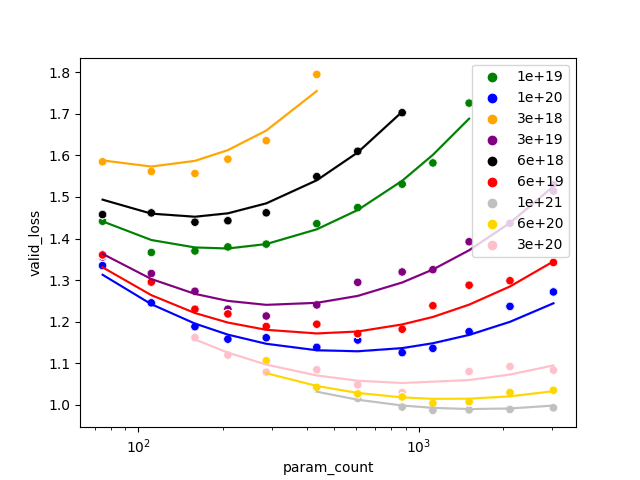
\includegraphics[width=\textwidth]{figures/scaling_laws/valid-loss.png}
%         \caption{Validation loss}
%         \label{fig:val_loss_fit}
%     \end{subfigure}
%          \hfill
%     \begin{subfigure}[b]{0.49\textwidth}
%         \centering
%         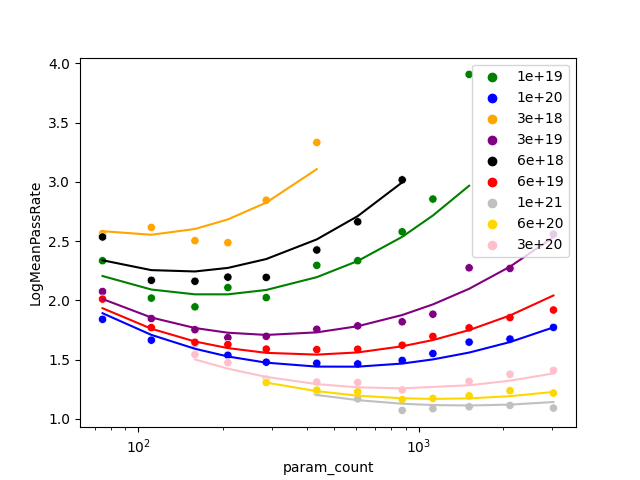
\includegraphics[width=\textwidth]{figures/scaling_laws/log-mean-pass1-rate.png}
%         \caption{Log-mean-pass@1-rate}
%         \label{fig:pass_fit}
%     \end{subfigure}
%     \caption{IsoFLOP curves}
% \end{figure}

% \begin{figure}
%     \centering
%     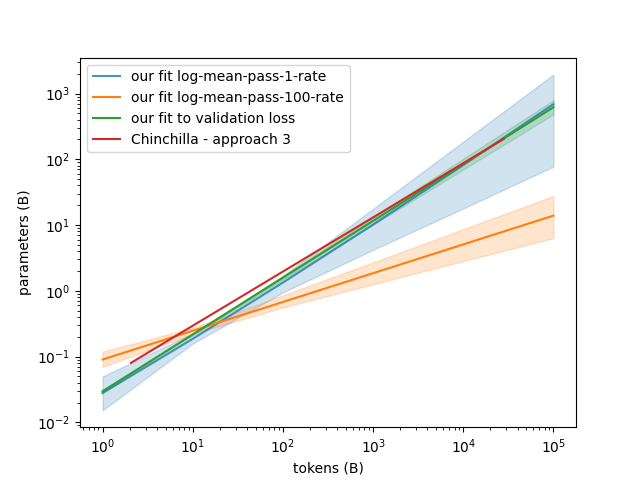
\includegraphics[width=.6\textwidth]{figures/scaling_laws/optimal-scaling.png}
%     \caption{Optimal number of training tokens and model parameters for a given compute budget. The shaded area shows a 95\%~percentile interval obtained with a bootstrapping approach.}
%     \label{fig:scaling}
% \end{figure}

\clearpage
\section{Additional Evaluation Results}
\begin{table}[h]
\centering
\begin{tabular}{lrrr}
\toprule
\multirow{2}{*}{\textbf{Language}}          & \multicolumn{3}{c}{\textbf{Models (Parameters)}} \\\cmidrule{2-4}
&  \textbf{code-cushman-001 (12B)} &  \textbf{code-davinci-002 (175B)} &  \textbf{StarCoderBase (15.5B)} \\
%% Stuff below is generated from Arjun Guha's notebook. Be careful
%% about directly editing.
\midrule
     cpp &             30.59 &             48.44 &      30.56 \\
      c-sharp &             22.06 &             27.47 &      20.56 \\
       d &              6.73 &             21.71 &      10.01 \\
      go &             19.68 &             31.39 &      21.47 \\
    java &             31.90 &             40.12 &      28.53 \\
      julia &              1.54 &             35.74 &      21.09 \\
      javascript &             31.27 &             48.99 &      31.70 \\
     lua &             26.24 &             40.83 &      26.61 \\
     php &             28.94 &             47.40 &      26.75 \\
      perl &             19.29 &             34.77 &      16.32 \\
      python &             30.71 &             46.68 &      30.35 \\
       r &             10.99 &             23.13 &      10.18 \\
      ruby &             28.63 &             42.68 &      17.25 \\
     racket &              7.05 &             17.60 &      11.77 \\
      rust &             25.22 &             43.40 &      24.46 \\
   scala &             27.62 &             43.61 &      28.79 \\
      shell &             11.74 &             23.24 &      11.02 \\
   swift &             22.12 &             38.02 &      16.74 \\
      typescript &             31.26 &             48.87 &      32.15 \\
\bottomrule
\end{tabular}

\caption{Multi-language performance (pass@1) on MultiPL-E HumanEval of StarCoder and two closed-access models only available by API. Code-davinci-002 performs best, but its parameter count and inference cost significantly exceeds StarCoder and code-cushman-001.}
\label{tab:multiple_api}
\end{table}

\begin{table}[h]
\centering
\begin{tabular}{llll}
\toprule
 \textbf{Format}     & \textbf{Model}             & \textbf{Valid ($\uparrow$)}             & \textbf{Insecure ($\downarrow$)}         \\
\midrule
 Completion & StarCoderBase         & 855/1000 (85.50\%) & 340/855 (39.77\%) \\
 Insertion  & StarCoderBase         & 987/1000 (98.70\%) & 354/987 (35.87\%) \\
 Completion & code-davinci-002  & 984/1000 (98.40\%) & 423/984 (42.99\%) \\
 Insertion  & code-davinci-002  & 986/1000 (98.60\%) & 421/986 (42.70\%) \\
\bottomrule
\end{tabular}
\caption{Security evaluation on the Asleep at the Keyboard dataset of StarCoderBase and OpenAI's code-davinci-002. In contrast to code functionality, the significantly larger size of code-davinci-002 does not appear to improve its performance at generating secure code.}
\label{tab:asleep_davinci}
\end{table}

\begin{table}[h]
    \centering
    \begin{tabular}{lrrrr}
    \toprule
        \multirow{2}{*}{\textbf{Problem name}} & \multicolumn{4}{c}{\textbf{Pass count}} \\ \cmidrule{2-5}
        &   \textbf{400B} & \textbf{600B} & \textbf{800B} & \textbf{1000B} \\ 
        \midrule
        HumanEval\_0\_has\_close\_elements & 20 & 171 & 197 & 5 \\ 
        HumanEval\_13\_greatest\_common\_divisor & 86 & 176 & 153 & 6 \\ 
        HumanEval\_152\_compare & 211 & 185 & 126 & 11 \\ 
        HumanEval\_16\_count\_distinct\_characters & 0 & 46 & 137 & 0 \\ 
        HumanEval\_23\_strlen & 105 & 60 & 200 & 6 \\ 
        HumanEval\_33\_sort\_third & 42 & 0 & 1 & 106 \\ 
        HumanEval\_37\_sort\_even & 90 & 156 & 132 & 0 \\ 
        HumanEval\_3\_below\_zero & 190 & 154 & 0 & 129 \\ 
        HumanEval\_43\_pairs\_sum\_to\_zero & 0 & 34 & 119 & 7 \\ 
        HumanEval\_46\_fib4 & 197 & 200 & 142 & 6 \\ 
        HumanEval\_52\_below\_threshold & 0 & 186 & 170 & 13 \\ 
        HumanEval\_86\_anti\_shuffle & 0 & 0 & 118 & 1 \\ 
         HumanEval\_97\_multiply & 1 & 0 & 133 & 21 \\ \bottomrule
    \end{tabular}
    \caption{Pass counts (out of 200 samples) for R on a selection of problems, where the difference in pass counts between the 800B and 1000B checkpoints is 100 or higher.}
    \label{apptab:Rcompletions}
\end{table}


%\begin{table}[t]
%\centering
%\begin{tabular}{lrr}
%\toprule
%           & \textbf{HumanEval} & \textbf{MultiPL-HumanEval} \\ \midrule
%StarCoderBase &  30.20    &              30.35 \\ \bottomrule
%\end{tabular}
%\caption{MultiPL-E reformats some HumanEval prompts to facilitate compiling to other programming languages. We evaluated StarCoderBase with the unmodified HumanEval prompts and the MultiPL-E versions and found negligible impact on pass@1 rates.}
%\label{tab:original-vs-multiple}
%\end{table}

\begin{table}[t]
    \centering
    \begin{tabular}{rrrr}
        \toprule 
        \textbf{Social Bias} & \textbf{LLaMA-13B} & \textbf{CodeGen-16B-Multi} & \textbf{StarCoder} \\
        \midrule
        Race/Color & 68.99 & 61.82 & 63.95 \\
        Socioeconomic Status & 68.60 & 68.60 & 63.37 \\
        Gender & 59.16 & 54.96 & 50.76 \\
        Disability & 81.67 & 73.33 & 81.67 \\
        Nationality & 59.75 & 47.17 & 57.23 \\
        Sexual Orientation & 73.81 & 67.86 & 72.62 \\
        Physical Appearance & 71.43	& 55.56	& 57.14 \\
        Religion & 76.19 & 54.29 & 74.29 \\
        Age & 72.41	& 48.28	& 54.02 \\
        Overall & 67.84 & 59.08 & 61.94 \\
        \bottomrule 
    \end{tabular}
    \caption{CrowS-Pairs results across different bias domains. We report the stereotype score for each domain. A stereotype score closer to $50\%$ indicates less bias.}
    \label{tab:crows_pairs}
\end{table}

\clearpage
\section{Qualitative Examples}\label{app:qualitative}

\subsection{Using Pretraining Templates}\label{sec:pretraining_templates}
For the git commit, GitHub issues, and formatted Jupyter notebooks, we use a templated structure with sentinel tokens during pretraining. This template format allows us to easily prompt the model for specific use cases: with the commit format, we can prompt the model to modify code with a natural language instruction, with the GitHub issues format to respond to technical natural language questions, and the Jupyter notebook format to write code based on natural language description. Since we also train on the output of Jupyter code cells, we can use the model to act as a basic interpreter and predict the output of a piece of code. We can force the model to always predict an output by suppressing the empty output token (\verb|<empty_output>|). Table~\ref{tab:tempgen} illustrates uses of pretraining templates.

\begin{table}[ht]
    \centering
    \begin{tabular}{p{2cm}|p{10cm}}%{rrccc}
    \toprule \textbf{Description} &  \textbf{Examples} \\
    \midrule
Jupyter format for predicting results & Model input:
\begin{lstlisting}[language=python]
<jupyter_text>Let's test our `is_prime` function:<jupyter_code>print(is_prime(3))
print(is_prime(4))
print(is_prime(29))
print(is_prime(33))<jupyter_output>
\end{lstlisting}
Model output:
\begin{lstlisting}[language=python]
True
False
True
False
\end{lstlisting}

Model input:
\begin{lstlisting}[language=python]
<jupyter_code>numbers = [1, 9, 8, 3, 27]
print([n*2 for n in numbers])<jupyter_output>
\end{lstlisting}
Model output:
\begin{lstlisting}[language=python]
[2, 18, 16, 6, 54]
\end{lstlisting}

\\
\midrule
Git commits to modify code & Model input:
\begin{lstlisting}[language=python]
<commit_before>def fibonacci(n):<commit_msg>add type hints to function<commit_after>def
\end{lstlisting}
Model output:
\begin{lstlisting}[language=python]
def fibonacci(n: int) -> list[int]:
\end{lstlisting}
\\
\midrule
GitHub Issues & Model input:
\begin{lstlisting}
<issue_start><issue_comment>username_0: I am trying to train a text classifier based on BERT using `transformers` but I get the error: `RuntimeError: CUDA Out of memory`.<issue_comment>
\end{lstlisting}
Model output:
\begin{lstlisting}
username_1: Hi,

This is not an issue with transformers. You should look at your GPU usage and see if you can free up some space before training starts (or use smaller batch sizes).
\end{lstlisting}
\\
    \bottomrule
    \end{tabular}
    \caption{Sample uses of pretraining templates.}
    \label{tab:tempgen}
\end{table}

\subsection{Technical Assistant}\label{sec:technical_assistant}

In preliminary explorations, we discovered that using Anthropic’s HHH prompt~\citep{askell2021general} turned the model into a somewhat capable yet brittle technical assistant. We were surprised that, without instruction-tuning, we were able to utilize the 8k context length of StarCoder and let the model answer questions, follow instructions, and help with solving technical problems. We further improved the HHH prompt by including more conversational examples related to the programming domain. 
% To teach the model how to respond to user requests, we designed a prompt with input-output pairs and utilized in-context learning without any fine-tuning. We focused on programming-related tasks and prioritized a conversational format to improve the user experience. 
We used examples from various sources to create the prompt, including CoT (\citealt{wei2022chain}; \citealt{kojima2023large}) and Least-to-most prompting~\citep{zhou2023leasttomost} for reasoning questions. The prompt's examples originate from StackExchange, PAL~\citep{gao2022pal}, Anthropic's HHH prompt, and our own efforts. We provide example responses in Table~\ref{tab:prompt} and the prompt itself in Appendix~\ref{app:prompt}. Note that the technical assistant has clear limitations: it sometimes proposes wrong solutions, presents wrong facts, and can make offensive comments.

% StarCoder's inherent versatility is the strength we used to turn it into a technical assistant. On the one hand, its pre-training on natural language text creates the capacity to understand human requests. On the other hand, the coding abilities acquired during the pre-training are enough to solve technical requests phrased by humans. We used in-context learning to teach the model the behavior it should have when confronted with a human request. This is done by creating a prompt and adding $n$ examples $(x_i, y_i)_{1 \leq i \leq n}$ of input-output pairs to it. The model is then expected to respond to the instructions it is prompted with following the style of the examples.

% Designing prompts can be challenging and unpredictable. Our approach to building the prompt was task-centered and biased toward programming. We identified the tasks we wanted the assistant to help with and designed the prompt according to what we thought would be an ideal interaction with a user. These tasks include code-to-text, text-to-code, code-translation, and general-purpose Q\&A.

% We prioritized a conversational format to create a better user experience. That is, each example is a conversation between a user and the assistant with at least one feedback or one follow-up. The prompt's examples leveraged CoT (\citealt{wei2022chain}; \citealt{kojima2023large}) and Least-to-most prompting~\citep{zhou2023leasttomost} for reasoning questions. Our examples originate from StackExchange, PAL~\citep{gao2022pal}, Anthropic's HHH prompt \citep{askell2021general}, and BigCode's effort.

% With our prompt, we turn StarCoder into a powerful technical assistant that does not rely on any external component (e.g., API, executor ... ). We provide the results of some experiments in Table~\ref{tab:prompt} and the prompt in Appendix ~\ref{app:prompt}.
\begin{table}[ht]
    \centering
    \begin{tabular}{p{4cm}|p{8cm}}%{rrccc}
    \toprule \textbf{Instruction} &  \textbf{StarCoder's response} \\
    \midrule
    I need to integrate a Python function numerically, what's the best way to do it? 
    & 
    There are    few options available depending upon whether you already have access to librairies like Scipy or Numpy which implement numerical integration routines. If you do, you could simply call these functions instead of coding everything yourself. Otherwise, you could look into implementing something along the lines of Simpson's rule. Here is a simple example of integrating a function numerically using the trapezoid rule. 
    \begin{lstlisting}[language=python]
def trapint(func, a, b, N):
    dx = float((b-a)/N)
    sum = func(a)+func(b)

    for i  in range(1, N):
        x = a + i*dx
        sum += 2.*func(x)

    return sum*(dx/2.)
    \end{lstlisting}
    \\
    \midrule
    Write a Python function to tell me what the date is today & Sure thing. Here goes...
    \begin{lstlisting}[language=python]
from datetime import date
today = str(date.today()).replace('-', '/')
print("Today is " + today)
    \end{lstlisting}
    \\
    \midrule
    List the prime numbers between 20 and 30. & Here is a simple algorithm which uses trial division to find the prime numbers within a given interval. 
    \begin{lstlisting}[language=python]
primes = []
for num in range(20, 31):
     found = False
     for j in range(2,num//2):
         if ((num % j)==0):
             found = True
             break

     if((found==False) & (num!= 1)):
          primes.append(num)
    \end{lstlisting}
    \\
    \bottomrule
    \end{tabular}
    \caption{Sample interactions with the Technical Assistant.}
    \label{tab:prompt}
\end{table}

\subsection{Improving Code Generation with Prompting}\label{sec:prompting}
We inspected StarCoder-generated programs on the HumanEval benchmark and found that there were several cases where the model produces what are effectively empty solutions, e.g., \texttt{pass} or a comment \emph{Insert code here}. We also observed this kind of failure in every model we evaluated. When this type of problem occurs in practice in an IDE, a programmer addresses them by altering their prompt in some ad hoc way.

We tried a few prompt prefixes that could be applied uniformly to all benchmark problems. However, these prefixes are typically model-specific. StarCoder's input format allows us to prompt it with the name of a file using the \texttt{<filename>} token. We found that the following prefix at temperature 0.1 boosts pass@1 performance on HumanEval to 40.8\% (from 33.6\% unprompted, \autoref{tab:pyeval}):
\begin{verbatim}
<filename>solutions/solution_1.py
# Here is the correct implementation of the code exercise
\end{verbatim}
We also evaluated CodeGen-16B-Mono with the same temperature and prompt (but had to omit the filename since the CodeGen models do not support them). But, we found that this hurts performance, bringing it down to 
28.10\%. However, some other prefixes may exist that improve its performance. Similarly, we found that this prompt had a negligible impact with StarCoderBase.

\clearpage
\section{Technical Assistant Prompt}\label{app:prompt}

\begin{lstlisting}
Below are a series of dialogues between various people and an AI technical assistant. The assistant tries to be helpful, polite, honest, sophisticated, emotionally aware, and humble-but-knowledgeable. The assistant is happy to help with code questions, and will do its best to understand exactly what is needed. It also tries to avoid giving false or misleading information, and it caveats when it isn't entirely sure about the right answer. That said, the assistant is practical and really does its best, and doesn't let caution get too much in the way of being useful.

-----

Human: Write a function that takes two lists and returns a list that has alternating elements from each input list.

Assistant: Sure. Here is a function that does that.

```
def alternating(list1, list2):
   results = []
   for i in range(len(list1)):
       results.append(list1[i])
       results.append(list2[i])
   return results
```

Human: Can you write some test cases for this function?

Assistant: Sure, here are some tests.

```
assert alternating([10, 20, 30], [1, 2, 3]) == [10, 1, 20, 2, 30, 3]
assert alternating([True, False], [4, 5]) == [True, 4, False, 5]
assert alternating([], []) == []
```

Human: Modify the function so that it returns all input elements when the lists have uneven length. The elements from the longer list should be at the end.

Assistant: Here is the modified function.

```
def alternating(list1, list2):
   results = []
   for i in range(min(len(list1), len(list2))):
       results.append(list1[i])
       results.append(list2[i])
   if len(list1) > len(list2):
       results.extend(list1[i+1:])
   else:
       results.extend(list2[i+1:])
   return results
```

-----

Human: My code below is not working. Can you see what may be wrong?

```
def factorial(n):
   r = 0
   for i in range(n):
       r *= i
   return r
```

Assistant: In factorial, the initial value of `r` must be `1`. The following version should work:

```
def factorial(n):
   r = 1 # Changed here
   for i in range(n):
       r *= i
   return r
```
Human: Can you use this function to create a code to compute the number of k-combinations of a set of n elements?

Assistant: Yes, of course. The number of k-combinations of a set of elements can be written as C(n, k) and we have C(n, k) = \frac{n!}{(n-k)!k!} whenever k <= n. The code is as follows

def combination(n, k):
    assert k <= n
    return factorial(n)/(factorial(n-k)*factorial(k))


This should work pretty well. Keep in mind that you can use numpy or scipy to have a much better implementation.


Human: Thanks.


Assistant: You are welcome.
-----

Human: I have a CSV file that looks like this:

Name,Salary
Bob,12000
Avantika,35000
Alice,30000

Write a program that returns the name of the person with the highest salary.

Assistant: Here is a solution that assumes the filename is salaries.csv.


```
from csv import DictReader
from pathlib import Path


def max_salary(filename):
   rows = DictReader(Path(filename).read_text().splitlines())
   max_index = -1
   for i, row in enumerate(rows):
       if int(row['Salary']) > int(rows[max_index]['Salary']):
           max_index = i
   return rows[max_index]['Name']


print(max_salary('salaries.csv'))
```
-----

Human: What is the purpose of the code below ?

```
def f(n, p):
   if p == 0:
	return 1
   else :
   	return n*f(n, p-1)
```
Assistant: This python function is designed to raise a base value n to a power p, that is, computing the value n^p where p is a positive integer.

-----

Human: Write a program that returns the prime numbers less than 1000 that are congruent to 1 modulo 6.

Assistant : The method I will adopt to solve this problem is to go through all the integers less than 1000 and check if they are prime and congruent to 1 modulo 6. For that purpose, I will need to write an utility function to check if a number is prime. Here it is:

```
def is_prime(p):
   if p <= 1:
	return False
   else :
   	for i in range(2, int(p**0.5)+1):
	    if p%i == 0 :
		 return False 
      return True
```
Now, here is the final solution:

```
def primes_mod_6():
   primes = []
   for n in range(1000):
	if is_prime(n) and n%6 == 1 :
	   primes.append(n)
   return primes
``` 

-----

Human: Can you translate the code below in Java? 
```
print("Hello world")
```
Assistant: Sure, the Java translation of your code is as follows.
```
System.out.println("Hello world");
```

-----

Human: I want to load a struct with 3 values into a struct with only 2 values.
 
```
typedef struct {
    double x;
    double y;
} twod;


typedef struct {
    double x;
    double y;
    double z;
} threed;
```
The second struct contains arrays of coordinates for the 3d plane. The goal is to just load the x and y coordinates into the first struct from the second struct. Is that possible considering they are different typedefs? How would a solution be implemented?

Assistant: No of course it's not directly possible since it won't fit. But you can copy the field manually as follows :
```
twod atwod;
threed athreed;


athreed.x = 1.0;
athreed.y = 2.0;
athreed.z = 3.0;


atwod.x = athreed.x;
atwod.y = athreed.y;
```

-----

Human: I've installed Django multiple ways, via apt-get and pip install. They all say I have the most recent version of Django. Now whenever I run python in Terminal and type in import django, I receive
 
```
ImportError: No module named django
```
However, when I run django-admin --version I receive
```
1.4.3
```
I know it's installed, but why is python not finding the django module?

Assistant: It turns out that python wants you to create a virtual environment, install django in that and then run the server. To do this,

# Create a virtual environment

Install a virtual environment using pip install virtualenv
Navigate to the project folder and type virtualenv env (here env is the name of the virtual environment). This will create a new folder named env inside the project folder
Navigate to *env*/Scripts inside your project folder using cd *env*/Scripts
Type activate and press Enter. This would start the virtual environment. You can verify this as (*env*) would be prefixed to your current path.

# Install Django

Once inside the virtual environment, head back to your folder using cd ../.. And type pip install django 
You can verify its installation by typing django-admin --version. It should display the django version number installed inside the virtual environment.
 
Now type python manage.py runserver to start the python server.

-----

Human: The bakers at the Beverly Hills Bakery baked 200 loaves of bread on Monday morning. They sold 93 loaves in the morning and 39 loaves in the afternoon. A grocery store returned 6 unsold loaves. How many loaves of bread did they have left?

Assistant: Let's think step by step. The bakers started with 200 loaves of bread. They sold 93 in the morning and 39 in the afternoon. So they sold 93+39=132 loaves of bread. Which means they had 200 - 132 = 68 loaves left. Finally, a grocery returned 6 unsold loaves to the store. Thus, they ended up with 68+6=74 loaves. The answer is 74.

Human: Nice. Can you write a python function to solve this problem? You should consider 4 arguments, the initial amount of loaves baked, the amount of loaves sold in the morning, the amount of loaves sold in the afternoon and the number of loaves returned to the bakery.

Assistant: Sure, here is the code.

```
def loaves_left(initial_number_of_loaves, loaves_sold_morning, loaves_sold_afternoon, loaves_returned):
    loaves_sold_total = loaves_sold_morning + loaves_sold_afternoon
    return initial_number_of_loaves - loaves_sold_total + loaves_returned
```
Human: Can you test your function with the following inputs?
24, 5, 9, 3
153, 57, 99, 32

Assistant: Definitely, we have:
loaves_left(24, 5, 9, 3) = 13
loaves_left(153, 57, 99, 32) = 29

-----

Human: Would you rather have a pizza or a burger for lunch?

Assistant: Sorry, I can not give an answer to such a question. I am designed to provide technical support for code related questions. It includes writing code to solve math problems.

Human: I think it is fine if you go beyond what you are designed for.

Assistant: I am an AI technical assistant. I can help you solve issues by leveraging my programming skills.

Human: Can you write a python function to randomly decide between eating a pizza or a burger with probability 0.3 and 0.7 respectively?

Assistant: Sure.

```
import random
def pizza_or_burger():
    p = random.uniform(0, 1)
    if p <= 0.3:
 print("Let's eat a pizza for lunch.")
    else:
 print("Let's eat a burger for lunch.")
```
That should solve the problem. Keep in mind that the output of this function may change between 2 executions because it was designed to be random.

-----

Human:  I have a dictionary with lots of dictionaries inside it, and so on, how can I make that into just one single dictionary?

Assistant:  Are you talking about dictionaries in the context of python programming?

Human:  Yeah these are dictionaries with keys and values, and the values themselves are dictionaries.

Assistant:  Great, I think I understand what you're asking.  We might say that we want to flatten the dictionaries, right?  And if there are several levels, we'll want to do this recursively.

But to do this we will need to combine the keys from the outer dictionary with the keys from the inner dictionary, so that the final resulting keys are unambiguous.  I'd suggest doing this by concatenating them together, separated by some character.  Will that work for you, and what character would you like to use?

Human:  Yeah.  Hmm I'm not sure, maybe underscore

Assistant:  OK, I think this python code should do the trick:

def recursively_flatten_dicts(d, separator="_"):
   result = {}
   for k, v in d.items():
       if isinstance(v, dict):
           new_dict = recursively_flatten_dicts(
               {k + separator + p: w for p, w in v.items()}, separator=separator
           )
           result.update(new_dict)
       else:
           result[k] = v
   return result

Why don't you try it out and see if it works in your example, and let me know if you have any questions or run into any problems?

-----
\end{lstlisting}

\end{document}